\documentclass[20pt,a4paper]{report}

\usepackage{fontspec}
\usepackage{polyglossia}
\setmainlanguage{english}
\setotherlanguage{bengali}

\setmainfont{Times New Roman}
\newfontfamily\bengalifontR[Script=Bengali]{Kohinoor Bangla}
\newfontfamily\bengalifontB[Script=Bengali]{Kohinoor Bangla Bold}

\makeatletter
\newcommand{\savedFontCmd}{}
\newcommand{\bengalienter}{%
  \edef\savedFontCmd{%
    \noexpand\fontencoding{\f@encoding}%
    \noexpand\fontfamily{\f@family}%
    \noexpand\fontseries{\f@series}%
    \noexpand\fontshape{\f@shape}%
    \noexpand\selectfont}%
  \expandafter\ifx\csname f@series\endcsname\bfdefault
    \bengalifontB
  \else
    \bengalifontR
  \fi
}
\newcommand{\bengalileave}{\savedFontCmd}
\makeatother

\usepackage{ucharclasses}
\setTransitionsFor{Bengali}{\bengalienter}{\bengalileave}

\usepackage{newunicodechar}
\newunicodechar{।}{{\bengalifontR ।}}
\newunicodechar{॥}{{\bengalifontR ॥}}

\usepackage{graphicx}
\usepackage{url}
\usepackage{ulem}
\providecommand{\ul}[1]{\uline{#1}}
\usepackage[hidelinks]{hyperref}
\usepackage{longtable}
\usepackage{array}
\usepackage{booktabs}
\usepackage{calc}
\usepackage{caption}
\newcounter{none}

\providecommand{\tightlist}{%
  \setlength{\itemsep}{0pt}\setlength{\parskip}{0pt}}

\setlength{\parindent}{0pt}
\setlength{\parskip}{6pt}
\spaceskip=0.5em plus 0.3em minus 0.1em
\linespread{1.7}

\usepackage[margin=1in]{geometry}

\makeatletter
\def\bnglnum#1{\expandafter\bngl@num\number\csname c@#1\endcsname\@empty}
\def\bngl@num#1{\ifx\@empty#1\else\bngl@digit{#1}\expandafter\bngl@num\fi}
\def\bngl@digit#1{\ifcase#1 ০\or ১\or ২\or ৩\or ৪\or ৫\or ৬\or ৭\or ৮\or ৯\fi}
\makeatother

\renewcommand{\thesection}{\bnglnum{section}}
\renewcommand{\thesubsection}{\thesection.\bnglnum{subsection}}
\renewcommand{\thesubsubsection}{\thesubsection.\bnglnum{subsubsection}}

\addto\captionsenglish{\renewcommand{\contentsname}{সূচিপত্র}}

\title{অনাহারকে অস্ত্র হিসেবে ব্যবহার: গাজা যুদ্ধের একটি কেস স্টাডি}
\author{কল্যান রায় \and মোছাঃ আসমা খাতুন}
\date{এপ্রিল, ২০২৬}

\begin{document}

\begin{titlepage}
\centering

{\bfseries\large অনাহারকে অস্ত্র হিসেবে ব্যবহার: গাজা যুদ্ধের একটি কেস স্টাডি\newline STARVATION IS A WEAPON: A CASE STUDY OF THE GAZA WAR\par}

\vspace{1em}

\includegraphics[width=2.37942in,height=2.09085in]{media/media/image1.png}

\vspace{1em}
{\bfseries কোর্স কোড: HIS-4206\par}

\vspace{0.5em}
{\bfseries বিএ (সম্মান) প্রজেক্ট পেপার\par}

\vspace{0.5em}
পাবনা বিজ্ঞান ও প্রযুক্তি বিশ্ববিদ্যালয়ের ইতিহাস বিভাগের বিএ(সম্মান) ডিগ্রির\\
শর্তপূরণের (আংশিক) জন্য উপস্থাপিত

\vspace{1em}
\textbf{\ul{তত্ত্বাবধায়ক}}\\[0.3em]
মো: শফিকুর রহমান\\
সহযোগী অধ্যাপক\\
ইতিহাস বিভাগ\\
পাবনা বিজ্ঞান ও প্রযুক্তি বিশ্ববিদ্যালয়

\vspace{2.5em}
\textbf{\ul{গবেষণা শিক্ষার্থী}}\\[0.8em]
\noindent\begin{minipage}[t]{0.44\textwidth}


\textbf{কল্যান রায়}\\[0.4em]
\raggedright
\begin{tabular}{@{}ll@{}}
রোল: ২০২০২৯\\
রেজি: ১২০৫১৭৪\\
শিক্ষাবর্ষ: ২০১৯-২০২০\\
\end{tabular}
\end{minipage}%
\hspace{0.08\textwidth}%
\begin{minipage}[t]{0.44\textwidth}
\textbf{মোছাঃ আসমা খাতুন}\\[0.4em]
\raggedright
\begin{tabular}{@{}ll@{}}
রোল: ২০২০৪৬\\
রেজি: ১২০৫১৯১\\
শিক্ষাবর্ষ: ২০১৯-২০২০\\
\end{tabular}
\end{minipage}

\vfill

{\bfseries ইতিহাস বিভাগ\par}
মানবিক ও সামাজিক বিজ্ঞান অনুষদ\\
পাবনা বিজ্ঞান ও প্রযুক্তি বিশ্ববিদ্যালয়, পাবনা

\vspace{0.5em}
{\bfseries এপ্রিল, ২০২৬\par}

\end{titlepage}

\clearpage
\section*{অঙ্গীকারনামা}
\addcontentsline{toc}{section}{অঙ্গীকারনামা}
\markboth{অঙ্গীকারনামা}{}

\vspace{1em}
আমরা পাবনা বিজ্ঞান ও প্রযুক্তি বিশ্ববিদ্যালয়ের ইতিহাস বিভাগের ২০১৯-২০২০ শিক্ষাবর্ষের নিয়মিত শিক্ষার্থী কল্যান রায় (রোল: ২০২০২৯, রেজি: ১২০৫১৭৪), মোছাঃ আসমা খাতুন (রোল: ২০২০৪৬, রেজি: ১২০৫১৯১) এই মর্মে অঙ্গীকার করছি যে, \textbf{``অনাহারকে অস্ত্র হিসেবে ব্যবহার : গাজা যুদ্ধের একটি কেস স্টাডি''} শিরোনামে সম্পন্ন প্রজেক্ট পেপারটি আমাদের নিজস্ব গবেষণা এবং এর কোনো অংশবিশেষ কোনো ডিগ্রি অর্জনের জন্য বা প্রকাশনার জন্য অন্য কোথাও জমা দেওয়া হয়নি।

\vspace{2em}

\noindent\begin{minipage}[t]{0.48\textwidth}
\raggedright
কল্যান রায়\\
রোল: ২০২০২৯\\
রেজি: ১২০৫১৭৪\\
শিক্ষাবর্ষ: ২০১৯-২০২০
\end{minipage}%
\hfill
\begin{minipage}[t]{0.48\textwidth}
\raggedleft
মোছাঃ আসমা খাতুন\\
রোল: ২০২০৪৬\\
রেজি: ১২০৫১৯১\\
শিক্ষাবর্ষ: ২০১৯-২০২০
\end{minipage}

\vspace{2em}

\begin{center}
ইতিহাস বিভাগ\\
মানবিক ও সামাজিক বিজ্ঞান অনুষদ\\
পাবনা বিজ্ঞান ও প্রযুক্তি বিশ্ববিদ্যালয়, পাবনা
\end{center}

\clearpage
\section*{প্রত্যয়নপত্র}
\addcontentsline{toc}{section}{প্রত্যয়নপত্র}
\markboth{প্রত্যয়নপত্র}{}

\vspace{1em}
প্রত্যয়ন করা যাচ্ছে যে, কল্যান রায় (রোল: ২০২০২৯, রেজি: ১২০৫১৭৪, শিক্ষাবর্ষ: ২০১৯-২০২০), মোছাঃ আসমা খাতুন (রোল: ২০২০৪৬, রেজি: ১২০৫১৯১, শিক্ষাবর্ষ: ২০১৯-২০২০) এর \textbf{``অনাহারকে অস্ত্র হিসেবে ব্যবহার : গাজা যুদ্ধের একটি কেস স্টাডি''} শিরোনামে গবেষণা প্রজেক্টটি আমার তত্ত্বাবধানে সম্পন্ন হয়েছে। এর কোনো অংশবিশেষ কোনো ডিগ্রি অর্জনের জন্য বা প্রকাশনার জন্য অন্য কোথাও জমা দেওয়া হয়নি। প্রজেক্টটি কর্তৃপক্ষের নিকট জমা প্রদানের জন্য অনুমোদন করা হলো।

\vspace{3em}

\begin{flushright}
\begin{minipage}{0.5\textwidth}
\raggedleft
\rule{5cm}{0.4pt}\\[0.3em]
\textbf{মো: শফিকুর রহমান}\\
সহযোগী অধ্যাপক\\
ইতিহাস বিভাগ\\
পাবনা বিজ্ঞান ও প্রযুক্তি বিশ্ববিদ্যালয়\\
পাবনা-৬৬০০
\end{minipage}
\end{flushright}

\clearpage
\section*{কৃতজ্ঞতানামা}
\addcontentsline{toc}{section}{কৃতজ্ঞতানামা}
\markboth{কৃতজ্ঞতানামা}{}

\vspace{1em}
``অনাহারকে অস্ত্র হিসেবে ব্যবহার : গাজা যুদ্ধের একটি কেস স্টাডি'' শিরোনামে রচিত গবেষণা প্রজেক্টটি পাবনা বিজ্ঞান ও প্রযুক্তি বিশ্ববিদ্যালয়ের ইতিহাস বিভাগের সহযোগী অধ্যাপক মো: শফিকুর রহমান স্যারের প্রত্যক্ষ তত্ত্বাবধান, অনুপ্রেরণা, সামগ্রিক সহযোগিতা, পরামর্শ ও দিকনির্দেশনায় সম্পন্ন হয়েছে। প্রজেক্টটি বাস্তবায়নের ক্ষেত্রে তিনি আমাদেরকে সর্বাত্মকভাবে সহায়তা করেছেন। তাঁর সহায়তা ছাড়া এই গবেষণা কর্ম রূপায়ণ করা আমাদের পক্ষে সম্ভব হতো না। প্রজেক্টের শুরু থেকে শেষ পর্যন্ত সার্বিক উৎসাহ, উপদেশ, সাহায্য-সহযোগিতা ও দিকনির্দেশনা সকল প্রশংসার ঊর্ধ্বে। আমরা আমাদের তত্ত্বাবধায়ক স্যারের কাছে বিশেষভাবে কৃতজ্ঞতা প্রকাশ করছি।

ইতিহাস বিভাগের চেয়ারম্যান ড. মো: হাবিবুল্লাহ্ স্যারের প্রতি বিশেষ কৃতজ্ঞতা জ্ঞাপন করছি, যিনি সর্বদা আমাদের গবেষণার কাজের অগ্রগতি সম্পর্কে খোঁজ খবর নিয়েছেন, গবেষণা কর্ম সম্পন্ন করতে উৎসাহ, অনুপ্রেরণা ও তাগিদ দিয়েছেন এবং গবেষণা উপকরণ দিয়ে বিভিন্ন সময় সহযোগিতা করেছেন। আমরা আন্তরিকভাবে কৃতজ্ঞতা জানাই পাবনা বিজ্ঞান ও প্রযুক্তি বিশ্ববিদ্যালয়ের ইতিহাস বিভাগের সহযোগী অধ্যাপক মো: শফিকুর রহমান স্যার, সহকারী অধ্যাপক মোছা: রাহেনা বেগম ম্যাম, সহকারী অধ্যাপক মোছাঃ শাহানাজ পারভীন ম্যাম, প্রভাষক ফারুক গাজী স্যার, প্রভাষক আবু তায়েব ও প্রভাষক আফরিন জাহান ম্যাম এবং সিনিয়র অফিস সহকারী সাকিবুর রহমান ভাই-এর প্রতি। গবেষণা সম্পন্ন করার ক্ষেত্রে সার্বিকভাবে সহযোগিতা করেছে আমাদের সহপাঠী এবং সিনিয়র ভাই-আপুরা। তাদের প্রতি অশেষ কৃতজ্ঞতা জ্ঞাপন করছি।

পরিশেষে, পাবনা বিজ্ঞান ও প্রযুক্তি বিশ্ববিদ্যালয়ের গ্রন্থাগার, ইতিহাস বিভাগের গ্রন্থাগার, শ্রদ্ধার সাথে স্মরণ করছি আমাদের পিতামাতা, পরিবার, বন্ধু-বান্ধব ও শুভাকাঙ্ক্ষীদের, যারা গবেষণাকর্মটি সম্পাদন করতে সার্বক্ষণিক উৎসাহ ও প্রেরণা দানের মাধ্যমে আমাদের সহযোগিতা করেছেন। সাবধানতা অবলম্বন করা সত্ত্বেও গবেষণা কর্মটিতে কিছু ত্রুটি-বিচ্যুতি থাকতে পারে, এজন্য আমরা আন্তরিকভাবে ক্ষমাপ্রার্থী। সর্বোপরি, এই প্রজেক্টটি সমাপ্ত করতে পেরে আমরা আনন্দিত এবং মহান আল্লাহ তায়ালার নিকট শুকরিয়া জ্ঞাপন করছি।

\clearpage
\section*{সারসংক্ষেপ}
\addcontentsline{toc}{section}{সারসংক্ষেপ}
\markboth{সারসংক্ষেপ}{}

\vspace{1em}
আলোচ্য গবেষণাপত্রটি গাজা সংঘাতের প্রেক্ষাপটে বেসামরিক জনগণের বিরুদ্ধে ``অনাহারকে যুদ্ধপদ্ধতি হিসেবে ব্যবহার'' বিষয়টির একটি সমন্বিত, প্রমাণভিত্তিক এবং আইনি বিশ্লেষণ উপস্থাপন করে। গাজা উপত্যকা দীর্ঘদিন ধরে অবরোধ, সামরিক অভিযান এবং রাজনৈতিক নিয়ন্ত্রণের অধীনে থাকায় সেখানে একটি জটিল মানবিক সংকটের সৃষ্টি হয়েছে, যা ২০২৩ সালের পরবর্তী সংঘাতে আরও তীব্র আকার ধারণ করে। খাদ্য, পানি, জ্বালানি এবং চিকিৎসা সহায়তার প্রবেশে ধারাবাহিক ও কাঠামোগত বিধিনিষেধ, পাশাপাশি বেসামরিক অবকাঠামোর ব্যাপক ধ্বংস, গাজার জনগণের জীবনধারণের মৌলিক উপকরণকে মারাত্মকভাবে ক্ষতিগ্রস্ত করেছে। এই বাস্তবতায় অনাহারকে কেবল একটি মানবিক বিপর্যয় হিসেবে নয়, বরং একটি সম্ভাব্য কৌশলগত যুদ্ধপদ্ধতি হিসেবে মূল্যায়নের প্রয়োজনীয়তা দেখা দিয়েছে।

এই গবেষণার মূল উদ্দেশ্য হলো নির্ধারণ করা যে, গাজায় গৃহীত সামরিক ও প্রশাসনিক পদক্ষেপগুলো কি কেবল বৈধ সামরিক প্রয়োজনীয়তার অংশ, নাকি সেগুলো বেসামরিক জনগণের ওপর পরিকল্পিতভাবে অনাহার আরোপের একটি সুসংগঠিত কৌশল। এ লক্ষ্যে গবেষণাটি আন্তর্জাতিক মানবিক আইন, আন্তর্জাতিক মানবাধিকার আইন এবং আন্তর্জাতিক ফৌজদারি আইনের আলোকে ঘটনাবলীর বিশ্লেষণ করেছে। বিশেষভাবে জেনেভা কনভেনশন, রোম সংবিধি এবং সংশ্লিষ্ট আন্তর্জাতিক আইনি কাঠামোর বিধানসমূহ ব্যবহার করে অনাহারকে যুদ্ধপদ্ধতি হিসেবে ব্যবহারের বৈধতা ও দায়বদ্ধতা মূল্যায়ন করা হয়েছে। গবেষণাটি একটি গুণগত পদ্ধতি অনুসরণ করে, যেখানে জাতিসংঘ, মানবাধিকার সংস্থা, আন্তর্জাতিক সংগঠন এবং নির্ভরযোগ্য সংবাদমাধ্যমের প্রতিবেদনসমূহ থেকে সংগৃহীত তথ্যকে থিম্যাটিক বিশ্লেষণের মাধ্যমে পর্যালোচনা করা হয়েছে।

গবেষণার ফলাফল থেকে প্রতীয়মান হয় যে, গাজায় খাদ্য ও জীবনধারণের অপরিহার্য উপকরণে প্রবেশাধিকার সীমিতকরণ, মানবিক সহায়তায় বাধা এবং অবকাঠামোগত ধ্বংস---এসব কার্যক্রম বিচ্ছিন্ন বা সাময়িক নয়; বরং একটি ধারাবাহিক ও কাঠামোগত প্রক্রিয়ার অংশ, যা বেসামরিক জনগণের ওপর গভীর ও দীর্ঘমেয়াদি প্রভাব সৃষ্টি করেছে। এই প্রক্রিয়াগুলো আন্তর্জাতিক মানবিক আইনের মৌলিক নীতির সঙ্গে সাংঘর্ষিক এবং প্রাসঙ্গিক আইনি মানদণ্ড অনুযায়ী এগুলো সম্ভাব্যভাবে যুদ্ধাপরাধ হিসেবে বিবেচিত হতে পারে। অতএব, এই গবেষণা গাজা সংঘাতকে একটি গুরুত্বপূর্ণ কেস স্টাডি হিসেবে উপস্থাপন করে, যা সমসাময়িক সশস্ত্র সংঘাতে বেসামরিক জনগণের সুরক্ষা, আন্তর্জাতিক আইনের কার্যকারিতা এবং জবাবদিহিতা নিশ্চিত করার প্রশ্নে একটি তাৎপর্যপূর্ণ অবদান রাখে।

\clearpage
\tableofcontents

\section{প্রথম অধ্যায়: ভূমিকা}\label{ux9aaux9b0ux9a5ux9ae-ux985ux9a7ux9afux9df-ux9adux9aeux995}

\subsection{১.১ গবেষণার প্রেক্ষাপট}\label{ux997ux9acux9b7ux9a3ux9b0-ux9aaux9b0ux995ux9b7ux9aaux99f}

ফিলিস্তিন মধ্যপ্রাচ্যের একটি ভূখণ্ড, যা দীর্ঘদিন ধরে ভূ-রাজনৈতিক, ঐতিহাসিক ও রাজনৈতিক সংঘাতের কেন্দ্রবিন্দু। এর অন্তর্ভুক্ত গাজা উপত্যকা একটি ঘনবসতিপূর্ণ ছোট উপকূলীয় অঞ্চল, যেখানে প্রায় ২০ লক্ষাধিক ফিলিস্তিনি বসবাস করে। ভৌগোলিকভাবে সীমিত হলেও গাজা রাজনৈতিক ও সামরিক সংঘাতের দিক থেকে অত্যন্ত গুরুত্বপূর্ণ। ২০০৭ সাল থেকে এটি কার্যত অবরুদ্ধ অবস্থায় রয়েছে, যেখানে স্থল, সমুদ্র ও আকাশপথে প্রবেশ ও প্রস্থানের উপর কঠোর নিয়ন্ত্রণ আরোপ করা হয়েছে। এই দীর্ঘস্থায়ী অবরোধ গাজাকে একটি গভীর মানবিক সংকটপূর্ণ অঞ্চলে পরিণত করেছে।

গাজা উপত্যকার সাম্প্রতিক সশস্ত্র সংঘাত, বিশেষ করে ২০২৩ সালের অক্টোবর থেকে শুরু হওয়া যুদ্ধ, এই অঞ্চলের সংকটকে এক নতুন মাত্রায় নিয়ে গেছে। হামাসের হামলার প্রতিক্রিয়ায় ইসরাইলের ব্যাপক সামরিক অভিযান, পূর্ণাঙ্গ অবরোধ ঘোষণা, এবং অবকাঠামো ধ্বংসের ফলে বেসামরিক জনগণের জীবনযাত্রা মারাত্মকভাবে বিপর্যস্ত হয়েছে। খাদ্য, পানি, বিদ্যুৎ, জ্বালানি ও চিকিৎসা সেবার প্রবেশ সীমিত বা বন্ধ হয়ে যাওয়ায় গাজায় একটি তীব্র মানবিক বিপর্যয় সৃষ্টি হয়েছে, যা আন্তর্জাতিক মহলে গভীর উদ্বেগের জন্ম দিয়েছে।

এই প্রেক্ষাপটে ``অনাহার'' কেবল একটি মানবিক সমস্যা নয়, বরং এটি একটি গুরুত্বপূর্ণ আইনি ও রাজনৈতিক প্রশ্নে পরিণত হয়েছে। ঐতিহ্যগতভাবে অনাহারকে প্রাকৃতিক দুর্যোগ বা অর্থনৈতিক ব্যর্থতার ফল হিসেবে দেখা হলেও, সমসাময়িক সংঘাতে এটি ক্রমশ একটি পরিকল্পিত ও কৌশলগত হাতিয়ার হিসেবে ব্যবহৃত হচ্ছে। যখন কোনো পক্ষ সচেতনভাবে খাদ্য, পানি ও অন্যান্য জীবনধারণের উপকরণে প্রবেশাধিকার সীমিত বা বন্ধ করে দেয়, তখন অনাহার একটি ``নীরব কিন্তু কার্যকর অস্ত্র'' হিসেবে কাজ করে, যা সরাসরি সামরিক আক্রমণ ছাড়াই একটি জনগোষ্ঠীকে দুর্বল করে দিতে সক্ষম।

আধুনিক আন্তর্জাতিক রাজনীতি ও সশস্ত্র সংঘাতের প্রকৃতি ক্রমাগত পরিবর্তিত হলেও যুদ্ধের সময় বেসামরিক জনগণের দুর্ভোগ একটি স্থায়ী ও গভীর সংকট হিসেবে রয়ে গেছে। বিশেষত সাম্প্রতিক দশকগুলোতে সশস্ত্র সংঘাতে বেসামরিক জনগণ সরাসরি লক্ষ্যবস্তুতে পরিণত হয়েছে, যেখানে সামরিক শক্তির পাশাপাশি খাদ্য, পানি, জ্বালানি ও চিকিৎসার মতো মৌলিক জীবনধারণের উপকরণগুলোকে নিয়ন্ত্রণ ও বঞ্চনার অস্ত্র হিসেবে ব্যবহার করা হচ্ছে। এই বাস্তবতায় অনাহার কেবল একটি মানবিক সংকট নয়, বরং একটি সুসংগঠিত যুদ্ধকৌশল হিসেবে আবির্ভূত হয়েছে।

আন্তর্জাতিক মানবিক আইন (International Humanitarian Law) স্পষ্টভাবে বেসামরিক জনগণের বিরুদ্ধে অনাহারকে যুদ্ধের পদ্ধতি হিসেবে ব্যবহার নিষিদ্ধ করেছে। জেনেভা কনভেনশন ও এর অতিরিক্ত প্রোটোকলসমূহে বেসামরিক জনগণের জীবন ও জীবিকা রক্ষাকে অগ্রাধিকার দেওয়া হলেও বাস্তব সংঘাত পরিস্থিতিতে এই বিধানসমূহ প্রায়ই উপেক্ষিত হয়। বিশেষ করে অবরোধ (blockade), ত্রাণ সহায়তায় বাধা, খাদ্য ও পানির অবকাঠামো ধ্বংস এবং জ্বালানি সরবরাহ বন্ধ করার মতো কৌশলগুলো বেসামরিক জনগণকে সমষ্টিগত শাস্তির মুখোমুখি করে।

গাজা উপত্যকার বর্তমান সংঘাত এই বাস্তবতার একটি সুস্পষ্ট উদাহরণ। দীর্ঘমেয়াদি অবরোধ ও সামরিক অভিযানের ফলে গাজার বেসামরিক জনগণ খাদ্য নিরাপত্তাহীনতা, অপুষ্টি, স্বাস্থ্যব্যবস্থার বিপর্যয় এবং ব্যাপক মানবিক সংকটের সম্মুখীন হয়েছে। বিভিন্ন আন্তর্জাতিক সংস্থার প্রতিবেদন অনুযায়ী, গাজায় খাদ্য, পানি ও চিকিৎসা সেবায় পরিকল্পিত ও কাঠামোগত বাধা সৃষ্টি হয়েছে, যা অনাহারকে একটি পদ্ধতিগত অস্ত্রে রূপ দিয়েছে।

যদিও আন্তর্জাতিক আইন সব ধরনের সশস্ত্র সংঘাতে অনাহারকে নিষিদ্ধ করে, তথাপি আন্তর্জাতিক অপরাধ আদালতের রোম সংবিধিতে বেসামরিক জনগণের অনাহারকে যুদ্ধাপরাধ হিসেবে স্বীকৃতি দেওয়া হয়েছে মূলত আন্তর্জাতিক সশস্ত্র সংঘাতের ক্ষেত্রে। এই সীমাবদ্ধতা আন্তর্জাতিক ফৌজদারি আইনে একটি গুরুত্বপূর্ণ ফাঁক সৃষ্টি করেছে, যা বাস্তব সংঘাত পরিস্থিতিতে জবাবদিহিতা প্রতিষ্ঠাকে দুর্বল করে। এই প্রেক্ষাপটেই সুইজারল্যান্ড কর্তৃক রোম সংবিধি সংশোধনের প্রস্তাব উত্থাপিত হয়, যাতে অ-আন্তর্জাতিক সশস্ত্র সংঘাতেও বেসামরিক জনগণের অনাহারকে যুদ্ধাপরাধ হিসেবে অন্তর্ভুক্ত করা যায়।

এই গবেষণা উক্ত প্রেক্ষাপটে গাজা সংঘাতে অনাহারকে যুদ্ধপদ্ধতি হিসেবে ব্যবহারের আইনি বিশ্লেষণ উপস্থাপন করে এবং আন্তর্জাতিক মানবিক আইন, আন্তর্জাতিক মানবাধিকার আইন ও আন্তর্জাতিক ফৌজদারি আইনের আলোকে এর বৈধতা ও দায়বদ্ধতা মূল্যায়ন করে।

\subsection{\texorpdfstring{\textbf{১.২} গবেষণার সমস্যা বিবৃতি}{১.২ গবেষণার সমস্যা বিবৃতি}}\label{ux997ux9acux9b7ux9a3ux9b0-ux9b8ux9aeux9b8ux9af-ux9acux9acux9a4}

গাজা উপত্যকায় চলমান মানবিক বিপর্যয়কে সাধারণভাবে একটি ত্রাণ-যোগ্য সংকট হিসেবে উপস্থাপন করা হলেও, বাস্তবে এটি আন্তর্জাতিক মানবিক আইন (International Humanitarian Law -- IHL) এবং আন্তর্জাতিক মানবাধিকার আইনের (International Human Rights Law -- IHRL) সম্ভাব্য গুরুতর ও পদ্ধতিগত লঙ্ঘনের একটি জটিল আইনি সমস্যা। বিশেষত বেসামরিক জনগণের খাদ্য, পানি, জ্বালানি ও চিকিৎসাসেবায় দীর্ঘস্থায়ী ও কাঠামোগত বাধা সৃষ্টি এই সংকটকে নিছক যুদ্ধের অনিচ্ছাকৃত পরিণতির পর্যায় ছাড়িয়ে একটি পরিকল্পিত নীতিগত কৌশলের প্রশ্নে উন্নীত করেছে।

এই গবেষণার কেন্দ্রীয় সমস্যা হলো ইসরাইলি বাহিনীর গাজায় পরিচালিত কর্মকাণ্ডের প্রকৃতি নির্ধারণ করা। প্রশ্নটি হলো---এই কর্মকাণ্ডগুলো কি কেবল হামাসের বিরুদ্ধে বৈধ সামরিক লক্ষ্য অর্জনের অংশ হিসেবে সংঘটিত হয়েছে, নাকি ফিলিস্তিনি বেসামরিক জনগণের জীবনধারণের উপকরণ ধ্বংস ও অনাহার সৃষ্টি করাই একটি সুস্পষ্ট ও ইচ্ছাকৃত যুদ্ধকৌশল হিসেবে ব্যবহৃত হয়েছে। এই পার্থক্য নির্ধারণ আন্তর্জাতিক আইনের দৃষ্টিতে অত্যন্ত গুরুত্বপূর্ণ, কারণ এটি সামরিক প্রয়োজনীয়তা (military necessity) ও যুদ্ধাপরাধ (war crime)--এর মধ্যকার সীমারেখা নির্ধারণ করে।

আলোচ্য সমস্যার যথাযথ মূল্যায়নের জন্য কয়েকটি মূল বিষয়ে অনুসন্ধান অপরিহার্য। প্রথমত, ইসরাইল কর্তৃক গাজায় খাদ্য, পানি, জ্বালানি ও মানবিক সহায়তার প্রবেশে আরোপিত বিধিনিষেধগুলো কি বিচ্ছিন্ন বা সাময়িক পদক্ষেপ, নাকি সেগুলো একটি ধারাবাহিক কৌশলগত প্যাটার্ন ও উচ্চপর্যায়ের নির্দেশনার ফল। দ্বিতীয়ত, এসব পদক্ষেপ আন্তর্জাতিক মানবিক আইন, বিশেষ করে বেসামরিক জনগণের বিরুদ্ধে অনাহারকে যুদ্ধপদ্ধতি হিসেবে নিষিদ্ধকারী বিধানগুলোর সঙ্গে কীভাবে সরাসরি সংঘর্ষে লিপ্ত হয়েছে। তৃতীয়ত, এই কৌশল বাস্তবায়নে ব্যবহৃত প্রাতিষ্ঠানিক কাঠামো, প্রশাসনিক নিয়ন্ত্রণ ও অবরোধ ব্যবস্থাগুলো কীভাবে বেসামরিক জনগণের ওপর সমষ্টিগত প্রভাব সৃষ্টি করেছে।

অতএব, এই গবেষণার মূল সমস্যা হলো গাজা যুদ্ধে ইসরাইলের কর্মকাণ্ড বিশ্লেষণ করে নির্ণয় করা যে বেসামরিক জনগণের অনাহার সৃষ্টি কি একটি অনিচ্ছাকৃত সামরিক পার্শ্বপ্রতিক্রিয়া, নাকি এটি একটি সুনির্দিষ্ট, পরিকল্পিত ও ইচ্ছাকৃত যুদ্ধকৌশল---যা আন্তর্জাতিক মানবিক আইন, আন্তর্জাতিক মানবাধিকার আইন এবং আন্তর্জাতিক ফৌজদারি আইনের অধীনে গুরুতর লঙ্ঘন হিসেবে বিবেচিত হতে পারে।

\subsection{\texorpdfstring{\textbf{১.৩ গবেষণা প্রশ্ন}}{১.৩ গবেষণা প্রশ্ন}}\label{ux997ux9acux9b7ux9a3-ux9aaux9b0ux9b6ux9a8}

সমসাময়িক সশস্ত্র সংঘাতে বেসামরিক জনগণের সুরক্ষা আন্তর্জাতিক আইনের অন্যতম মৌলিক নীতি হলেও বাস্তবে এই সুরক্ষা ক্রমশ চ্যালেঞ্জের মুখে পড়ছে। বিশেষত খাদ্য, পানি, জ্বালানি এবং চিকিৎসা সেবার মতো জীবনধারণের মৌলিক উপকরণে প্রবেশাধিকার সীমিত করার মাধ্যমে বেসামরিক জনগণকে দুর্বল করার প্রবণতা আধুনিক যুদ্ধকৌশলের একটি উদ্বেগজনক রূপ হিসেবে আবির্ভূত হয়েছে। গাজা উপত্যকার চলমান সংঘাত এই প্রবণতার একটি গুরুত্বপূর্ণ উদাহরণ, যেখানে আন্তর্জাতিক সংস্থা, মানবাধিকার সংগঠন এবং বিভিন্ন গবেষণায় বেসামরিক জনগণের বিরুদ্ধে অনাহারকে একটি সম্ভাব্য যুদ্ধপদ্ধতি হিসেবে ব্যবহারের অভিযোগ উত্থাপিত হয়েছে।

আন্তর্জাতিক মানবিক আইন স্পষ্টভাবে বেসামরিক জনগণের বিরুদ্ধে অনাহারকে যুদ্ধের পদ্ধতি হিসেবে ব্যবহার নিষিদ্ধ করে এবং জেনেভা কনভেনশন ও এর অতিরিক্ত প্রোটোকলসমূহে এই নিষেধাজ্ঞা সুপ্রতিষ্ঠিত। একইসঙ্গে, আন্তর্জাতিক অপরাধ আদালতের রোম সংবিধিতে (Rome Statute) নির্দিষ্ট প্রেক্ষাপটে অনাহারকে যুদ্ধাপরাধ হিসেবে স্বীকৃতি দেওয়া হয়েছে। তথাপি, বাস্তব সংঘাত পরিস্থিতিতে এই বিধানগুলোর প্রয়োগ, ব্যাখ্যা এবং প্রমাণনির্ভর মূল্যায়ন জটিল হয়ে ওঠে, বিশেষ করে যখন সামরিক প্রয়োজনীয়তা (military necessity) ও মানবিক সুরক্ষার মধ্যে ভারসাম্য নির্ধারণের প্রশ্ন সামনে আসে।

বর্তমান গবেষণার মূল সমস্যা এই প্রশ্নকে ঘিরে যে, গাজা সংঘাতে ইসরাইল কর্তৃক গৃহীত অবরোধ, মানবিক সহায়তায় বিধিনিষেধ, এবং খাদ্য, পানি ও জ্বালানি অবকাঠামোর ওপর আঘাত---এসব পদক্ষেপ কি বিচ্ছিন্ন ও সাময়িক সামরিক কৌশল, নাকি এগুলো একটি সুসংহত ও ধারাবাহিক নীতির অংশ, যার উদ্দেশ্য বেসামরিক জনগণের জীবনধারণের উপকরণ সীমিত করে অনাহার সৃষ্টি বা ত্বরান্বিত করা। এ বিষয়ে বিদ্যমান সাহিত্য ও প্রতিবেদনসমূহ মানবিক পরিস্থিতির অবনতি এবং খাদ্য নিরাপত্তাহীনতার মাত্রা তুলে ধরলেও, এই কর্মকাণ্ডগুলোর একটি সমন্বিত আইনি বিশ্লেষণ---যেখানে আন্তর্জাতিক মানবিক আইন, আন্তর্জাতিক মানবাধিকার আইন এবং আন্তর্জাতিক ফৌজদারি আইন একত্রে প্রয়োগ করা হয়---তুলনামূলকভাবে সীমিত।

এই গবেষণা সেই শূন্যস্থান পূরণের চেষ্টা করে, যেখানে গাজা সংঘাতের প্রেক্ষাপটে অনাহারকে যুদ্ধপদ্ধতি হিসেবে ব্যবহারের অভিযোগকে কেবল মানবিক বা রাজনৈতিক দৃষ্টিকোণ থেকে নয়, বরং একটি কঠোর আইনি কাঠামোর মধ্যে বিশ্লেষণ করা হবে। বিশেষত, এই গবেষণা অনুসন্ধান করবে যে উক্ত কর্মকাণ্ডগুলো আন্তর্জাতিক আইনের অধীনে ``starvation as a method of warfare'' হিসেবে শ্রেণিবদ্ধ হওয়ার জন্য প্রয়োজনীয় উপাদানসমূহ পূরণ করে কিনা, এবং এর ফলে উদ্ভূত সম্ভাব্য আন্তর্জাতিক অপরাধের দায়বদ্ধতা কীভাবে নির্ধারিত হতে পারে।

এই সমস্যার গুরুত্ব বহুমাত্রিক। প্রথমত, এটি আন্তর্জাতিক মানবিক আইনের কার্যকারিতা ও প্রয়োগযোগ্যতার প্রশ্নকে সামনে আনে। দ্বিতীয়ত, এটি যুদ্ধাপরাধের জবাবদিহিতা নিশ্চিত করার ক্ষেত্রে আন্তর্জাতিক ফৌজদারি আইনের সীমাবদ্ধতা ও সম্ভাবনাকে মূল্যায়নের সুযোগ সৃষ্টি করে। তৃতীয়ত, বেসামরিক জনগণের মৌলিক অধিকার সুরক্ষার ক্ষেত্রে আন্তর্জাতিক সম্প্রদায়ের ভূমিকা ও দায়িত্ব পুনর্বিবেচনার প্রয়োজনীয়তা তুলে ধরে। ফলে, এই বিষয়টি কেবল একটি নির্দিষ্ট সংঘাতের বিশ্লেষণ নয়, বরং সমসাময়িক আন্তর্জাতিক আইন ও নীতির জন্য একটি তাৎপর্যপূর্ণ পরীক্ষা ক্ষেত্র।

উপরোক্ত বিশ্লেষণের আলোকে এই গবেষণার কেন্দ্রীয় গবেষণা প্রশ্ন হলো:

গাজা যুদ্ধে ইসরাইলের সামরিক ও প্রশাসনিক পদক্ষেপ---বিশেষত অবরোধ আরোপ, মানবিক সহায়তার প্রবেশে বিধিনিষেধ, এবং জীবনধারণের জন্য অপরিহার্য অবকাঠামোর ধ্বংস---আন্তর্জাতিক মানবিক আইন ও আন্তর্জাতিক ফৌজদারি আইনের আলোকে কি বেসামরিক জনগণের বিরুদ্ধে অনাহারকে একটি পরিকল্পিত যুদ্ধপদ্ধতি হিসেবে ব্যবহারের পর্যায়ে উন্নীত হয়েছে, এবং যদি হয়ে থাকে, তবে এর জন্য আইনি দায়বদ্ধতা ও আন্তর্জাতিক জবাবদিহিতা কীভাবে নির্ধারণ করা যেতে পারে?

\subsection{\texorpdfstring{\textbf{১.৪ গবেষণার লক্ষ্য ও উদ্দেশ্য}}{১.৪ গবেষণার লক্ষ্য ও উদ্দেশ্য}}\label{ux997ux9acux9b7ux9a3ux9b0-ux9b2ux995ux9b7ux9af-ux993-ux989ux9a6ux9a6ux9b6ux9af}

উপর্যুক্ত গবেষণা প্রশ্নসমূহের আলোকে এই গবেষণার মুখ্য উদ্দেশ্য হলো গাজা যুদ্ধের প্রেক্ষাপটে ইসরাইল কর্তৃক বেসামরিক জনগণের বিরুদ্ধে অনাহারকে একটি যুদ্ধপদ্ধতি হিসেবে ব্যবহারের অভিযোগ আন্তর্জাতিক আইনের আলোকে একটি সুসংবদ্ধ, প্রমাণভিত্তিক এবং আইনিভাবে সঙ্গত বিশ্লেষণের মাধ্যমে মূল্যায়ন করা। এই সামগ্রিক উদ্দেশ্য বাস্তবায়নের লক্ষ্যে গবেষণাটি নিম্নলিখিত সুনির্দিষ্ট উদ্দেশ্যসমূহ অনুসরণ করবে:

\begin{itemize}
\item
  আন্তর্জাতিক মানবিক আইন, আন্তর্জাতিক মানবাধিকার আইন এবং আন্তর্জাতিক ফৌজদারি আইনের আলোকে ``অনাহারকে যুদ্ধপদ্ধতি হিসেবে ব্যবহার\textbf{''} ধারণাটির তাত্ত্বিক ও আইনি কাঠামো উপস্থাপন ও ব্যাখ্যা করা।
\item
  ইসরাইলি সামরিক ও রাজনৈতিক কর্তৃপক্ষের প্রকাশ্য বিবৃতি, নীতিগত সিদ্ধান্ত এবং মাঠপর্যায়ে পর্যবেক্ষিত কর্মকাণ্ডের ভিত্তিতে গাজায় অনাহার সৃষ্টি ও বজায় রাখার জন্য গৃহীত কৌশলসমূহ চিহ্নিত ও বিশ্লেষণ করা।
\item
  উক্ত কর্মকাণ্ডগুলোর সঙ্গে আন্তর্জাতিক মানবিক আইন (বিশেষত জেনেভা কনভেনশন ও এর অতিরিক্ত প্রোটোকলসমূহ) এবং আন্তর্জাতিক মানবাধিকার আইনের প্রাসঙ্গিক বিধানগুলোর তুলনামূলক বিশ্লেষণের মাধ্যমে সেগুলোর আইনি বৈধতা বা অবৈধতা নিরূপণ করা।
\item
  গাজায় বেসামরিক জনগণের ওপর এই কৌশলগুলোর ফলে সৃষ্ট মানবিক বিপর্যয়ের মাত্রা পরিসংখ্যানগত তথ্য ও গুণগত বর্ণনার মাধ্যমে নথিভুক্ত ও মূল্যায়ন করা।
\end{itemize}

\subsection{১.৫ গবেষণার প্রয়োজনীয়তা}\label{ux997ux9acux9b7ux9a3ux9b0-ux9aaux9b0ux9dfux99cux9a8ux9dfux9a4}

\subsubsection{১.৫.১ একাডেমিক প্রয়োজনীয়তা:}\label{ux98fux995ux9a1ux9aeux995-ux9aaux9b0ux9dfux99cux9a8ux9dfux9a4}

এই গবেষণা সমসাময়িক সশস্ত্র সংঘাত বিশ্লেষণে ``অনাহারকে যুদ্ধপদ্ধতি হিসেবে ব্যবহার'' ধারণাটিকে একটি সুস্পষ্ট কেস স্টাডির মাধ্যমে তাত্ত্বিক ও বিশ্লেষণাত্মকভাবে সমৃদ্ধ করবে। বিশেষত গাজা যুদ্ধের প্রেক্ষাপটে আন্তর্জাতিক মানবিক আইন, আন্তর্জাতিক মানবাধিকার আইন এবং আন্তর্জাতিক ফৌজদারি আইনের বিধানসমূহ একত্রে প্রয়োগ করে এই গবেষণা অনাহারকে কেবল মানবিক বিপর্যয় নয়, বরং একটি সম্ভাব্য যুদ্ধাপরাধ হিসেবে বিশ্লেষণের সুযোগ সৃষ্টি করবে।এছাড়া, এই গবেষণা যুদ্ধবিগ্রহ অধ্যয়ন (Conflict Studies), আন্তর্জাতিক আইন ও মানবাধিকার তত্ত্বের মধ্যে একটি গুরুত্বপূর্ণ আন্তঃশাস্ত্রীয় সংযোগ স্থাপন করবে। আইনগত বিশ্লেষণের পাশাপাশি মানবিক ও সামাজিক প্রভাবের মূল্যায়নের মাধ্যমে এটি একাডেমিক আলোচনায় একটি সমন্বিত দৃষ্টিভঙ্গি যোগ করবে

\subsubsection{১.৫.২ ব্যবহারিক/নীতিগত প্রয়োজনীয়তা:}\label{ux9acux9afux9acux9b9ux9b0ux995ux9a8ux9a4ux997ux9a4-ux9aaux9b0ux9dfux99cux9a8ux9dfux9a4}

ব্যবহারিক ও নীতিগত পর্যায়ে, এই গবেষণা নীতিনির্ধারক, কূটনীতিক, আন্তর্জাতিক সংস্থা এবং মানবিক সহায়তা প্রদানকারী সংস্থাসমূহের জন্য গাজা সংকটের অন্তর্নিহিত কাঠামোগত কারণ, আইনি দায়বদ্ধতা এবং জবাবদিহিতার প্রশ্নগুলো স্পষ্টভাবে অনুধাবনে সহায়ক হবে। বিশেষ করে অনাহারকে যুদ্ধকৌশল হিসেবে ব্যবহারের আইনি ফলাফল তুলে ধরার মাধ্যমে এটি ভবিষ্যৎ নীতিনির্ধারণ ও আন্তর্জাতিক প্রতিক্রিয়ার ক্ষেত্রে তথ্যভিত্তিক সিদ্ধান্ত গ্রহণে সহায়তা করতে পারে। একজন শিক্ষার্থী ও গবেষক হিসেবে, এই গবেষণা জটিল আন্তর্জাতিক ইস্যুতে গভীর অনুসন্ধান, সমালোচনামূলক চিন্তাভাবনা এবং প্রমাণভিত্তিক আইনি যুক্তি উপস্থাপনের দক্ষতা বিকাশে গুরুত্বপূর্ণ ভূমিকা পালন করবে। একই সঙ্গে এটি আন্তর্জাতিক আইন ও মানবাধিকার বিষয়ে গবেষণার ক্ষেত্রে একাডেমিক সক্ষমতা বৃদ্ধিতে অবদান রাখবে।

\subsection{\texorpdfstring{\textbf{১.৬} সাহিত্য পর্যালোচনা}{১.৬ সাহিত্য পর্যালোচনা}}\label{ux9b8ux9b9ux9a4ux9af-ux9aaux9b0ux9afux9b2ux99aux9a8}

এ্যালেক্স ডি ওয়াল (2018) যুক্তি দেখান যে আধুনিক দুর্ভিক্ষ প্রায়শই একটি "রাজনৈতিক অপরাধ" যেখানে খাদ্যকে জনগণকে দমনের হাতিয়ার হিসেবে ব্যবহার করা হয়। তার কাজ এই গবেষণার জন্য একটি মৌলিক কাঠামো দেয়, যাতে ইসরাইলের কর্মকাণ্ডকে শুধু সামরিক নয়, রাজনৈতিক নিয়ন্ত্রণের কৌশল হিসেবে দেখা যায় (\emph{Mass Starvation}, 2018.)।

জোহান গাল্টুং (1969)-এর তত্ত্ব গাজার দীর্ঘমেয়াদী অবরোধ ও অর্থনৈতিক নিষেধাজ্ঞাকে "কাঠামোগত সহিংসতা" হিসেবে ব্যাখ্যা করেছেন, যেখানে একটি জনগোষ্ঠীকে প্রাতিষ্ঠানিক ব্যবস্থার মাধ্যমে ধীরে ধীরে ধ্বংস করা হয় (Galtung, 1969a)।

আন্তর্জাতিক ফৌজদারি আদালতের রোম সংবিধি (1998) ইচ্ছাকৃতভাবে জনগণের জন্য জীবন রক্ষাকারী প্রয়োজনীয়তা বর্জন করাকে যুদ্ধাপরাধ হিসেবে তালিকাভুক্ত করে (\emph{Rome Statute of the International Criminal Court}, 2021)।

জাতিসংঘের ওচা (UN OCHA) রিপোর্ট অনুযায়ী, গাজায় খাদ্য নিরাপত্তাহীনতা কোনো সাময়িক সংকট নয়, বরং এটি একটি দীর্ঘমেয়াদি কাঠামোগত সমস্যায় পরিণত হয়েছে । গবেষকদের মতে, গাজার আকাশ, সমুদ্র এবং স্থলপথের ওপর পূর্ণ নিয়ন্ত্রণ থাকায় এখানে খাদ্য ও ওষুধের প্রবেশাধিকার সম্পূর্ণভাবে বাইরের শক্তির ওপর নির্ভরশীল (\emph{UN OCHA}, n.d.)।

World Food Programme (WFP)-এর ২০২৪ সালের মূল্যায়ন অনুযায়ী, গাজার ৯৫\% জনগণ তীব্র খাদ্য নিরাপত্তাহীনতায় ভুগছে, যার মধ্যে প্রায় ১১ লক্ষ মানুষ দুর্ভিক্ষ-সদৃশ পরিস্থিতির মধ্যে রয়েছে। সংস্থাটি সতর্ক করেছে যে ইসরাইলের সম্পূর্ণ অবরোধ ও খাদ্য অবকাঠামো ধ্বংসের ফলে গাজায় একটি "মনুষ্যসৃষ্ট দুর্ভিক্ষ" সৃষ্টি হয়েছে। WFP-এর মতে, মানবিক সাহায্য প্রবেশে কঠোর বাধা ও জ্বালানি নিষেধাজ্ঞার কারণে খাদ্য উৎপাদন ও বিতরণ ব্যবস্থা সম্পূর্ণ ধ্বংস হয়ে গেছে, যা আন্তর্জাতিক মানবিক আইনের সুস্পষ্ট লঙ্ঘন (\emph{WFP}, 2024.)

জাতিসংঘ শিশু তহবিল (UNICEF)-এর এপ্রিল ২০২৪ সালের প্রতিবেদন অনুযায়ী, গাজা সংঘাতে ৬৪,০০০-এরও বেশি শিশু নিহত বা আহত হয়েছে এবং ৫৬,০০০ শিশু এক বা উভয় পিতামাতা হারিয়েছে। সংস্থাটি সতর্ক করেছে যে ৫ বছরের কম বয়সী শিশুদের ৩১\% তীব্র অপুষ্টিতে ভুগছে, যা বিশ্বে সর্বোচ্চ হার। UNICEF-এর মতে, শিশুরা এখন "তিনটি থ্রেট"-এর মুখোমুখি: সরাসরি সহিংসতা, পানিবাহিত রোগের মহামারী এবং গণ-অনাহার, যা একটি প্রজন্মের শারীরিক ও মানসিক বিকাশকে স্থায়ীভাবে ক্ষতিগ্রস্ত করছে (\emph{UNICEF}, 2024.)

বিশ্ব স্বাস্থ্য সংস্থা (WHO) এর তথ্য অনুযায়ী, ২০২৩ সালের অক্টোবর থেকে শুরু হওয়া সংঘাত গাজার স্বাস্থ্য ব্যবস্থাকে প্রায় সম্পূর্ণরূপে ধ্বংস করে দিয়েছে। হাসপাতালগুলো ক্ষমতার চেয়ে অনেক বেশি রোগী ও বাস্তুচ্যুত নাগরিকের চাপে কার্যত অচল, যেখানে মাতৃত্বকালীন যত্ন থেকে দীর্ঘমেয়াদী রোগের চিকিৎসা পর্যন্ত সব ধরনের অপরিহার্য স্বাস্থ্যসেবা মারাত্মকভাবে বিঘ্নিত হয়েছে। সংস্থাটি সতর্ক করে দিয়ে বলেছে, বোমা হামলা, চিকিৎসা সামগ্রী, খাদ্য, পানি ও জ্বালানির চরম অভাব গাজার জনগণের স্বাস্থ্যগত বেঁচে থাকাকে হুমকির মুখে ফেলেছে, যা মানবিক বিপর্যয়ের দিকে দ্রুত এগিয়ে যাচ্ছে (\emph{WHO EMRO}, 2023.)

হিউম্যান রাইটস ওয়াচ (HRW) এর তথ্য অনুসারে, ইসরাইল ২০২৫ সাল জুড়ে লেবাননে বেসামরিক পুনর্নির্মাণ সরঞ্জাম ধ্বংস, পশ্চিম তীরে ফিলিস্তিনিদের জোরপূর্বক বাস্তুচ্যুতকরণ এবং অধিকৃত সিরিয়ায় গ্রামবাসীদের বিতাড়িত করার মাধ্যমে যুদ্ধাপরাধ সংঘটিত করছে। সংস্থাটি এসব কর্মকাণ্ডকে "স্পষ্ট যুদ্ধাপরাধ" ও "মানবতাবিরোধী অপরাধ" বলে অভিহিত করেছে এবং আন্তর্জাতিক সম্প্রদায়কে আইনি চাপ (স্যাংশন, বাণিজ্য পদক্ষেপ) বৃদ্ধি ও UNRWA-কে সমর্থন করার আহ্বান জানিয়েছে (\emph{HRW}, 2025.)

Amnesty International এর গাজা-সংক্রান্ত প্রতিবেদন অনুযায়ী, ইসরাইলি বাহিনী গাজার বেসামরিক জনগণ ও অবকাঠামোর উপর অস্বাভাবিক ও অসম হামলা চালিয়েছে, যা আন্তর্জাতিক মানবিক আইনের সুস্পষ্ট লঙ্ঘন। সংস্থাটি দাবি করে যে, ইসরাইল জেনেভা কনভেনশন ও রোম সংবিধি লঙ্ঘন করে হাসপাতাল, স্কুল, আশ্রয়কেন্দ্র এবং সাংবাদিকদের বাসস্থান ও অফিস লক্ষ্য করে হামলা চালিয়েছে, যা যুদ্ধাপরাধের মামলায় দায়ীদের বিচারের আওতায় আনার দাবি রাখে। অ্যামনেস্টি গাজার অবরোধকে "সমষ্টিগত শাস্তি" হিসেবে চিহ্নিত করেছে এবং আন্তর্জাতিক সম্প্রদায়কে অস্ত্র বিক্রয় বন্ধসহ ইসরাইলের বিরুদ্ধে জবাবদিহিতা নিশ্চিত করার পদক্ষেপ নিতে আহ্বান জানিয়েছে (\emph{Amnesty International}, n.d.)

অর্থনৈতিক, সামাজিক ও সাংস্কৃতিক অধিকার সংক্রান্ত জাতিসংঘ কমিটি (CESCR) তাদের মূল্যায়নে ইসরাইলকে দখলকৃত ফিলিস্তিনি ভূখণ্ডের জনগণের---বিশেষ করে গাজাবাসীর---অর্থনৈতিক, সামাজিক ও সাংস্কৃতিক অধিকার সুরক্ষা ও সম্মানের ব্যাপারে তার আন্তর্জাতিক আইনি বাধ্যবাধকতা পূরণে ব্যর্থ হওয়ার জন্য তীব্রভাবে সমালোচনা করেছে। কমিটি গাজার অবরোধকে অবৈধ, অকার্যকর ও অস্বাভাবিক করে তুলেছে, যা খাদ্য, স্বাস্থ্যসেবা, পানি, স্যানিটেশন ও শিক্ষার অধিকারের সুস্পষ্ট লঙ্ঘন। তাদের সিদ্ধান্ত হলো, ইসরাইলের নীতিগুলো অনেক ক্ষেত্রে ফিলিস্তিনিদের জীবনযাত্রার জন্য "কাঠামোগত বৈষম্য" তৈরি করে এবং আন্তর্জাতিক মানবাধিকার আইনের সরাসরি লঙ্ঘন (CESCR , n.d.)

২০২৩ সালের নভেম্বরে প্রকাশিত এই গবেষণাপত্রে সতর্ক করা হয়েছে যে, চলমান যুদ্ধ গাজায় অ্যান্টিমাইক্রোবিয়াল রেজিস্ট্যান্স (AMR) বা অ্যান্টিবায়োটিক-প্রতিরোধের একটি নীরব মহামারি সৃষ্টির দ্বারপ্রান্তে নিয়ে গেছে। গবেষণায় উঠে এসেছে যুদ্ধ-পূর্ব গাজার ৩৪\% হাসপাতালের পানিতেই অ্যান্টিবায়োটিক-প্রতিরোধী ব্যাকটেরিয়া ছিল, যুদ্ধের সময় আহতদের ক্ষেত্রে নির্দিষ্ট অ্যান্টিবায়োটিকের প্রতি প্রতিরোধ ৩০০\% বেড়েছে, এবং অ্যাল-আওদা হাসপাতালের ৭০\% নমুনায় বহু-ঔষধ-প্রতিরোধী ব্যাকটেরিয়া পাওয়া গেছে। (Moussally et al., 2023)

(Wilkin, 2025) এই গবেষণাপত্রটি পরীক্ষা করে দেখেছে যে, কীভাবে গাজায় চলমান যুদ্ধ পাশ্চাত্যের ভূ-সাংস্কৃতিক আধিপত্যকে (geocultural dominance) চ্যালেঞ্জের মুখে ফেলেছে। এটি দেখায় যে, সার্বজনীন উদারনৈতিক মূল্যবোধের (universal liberal values) প্রচারক হিসেবে পাশ্চাত্যের যে স্বীয় ভাবমূর্তি ছিল, তা এখন ক্রমবর্ধমানভাবে পর্যালোচনার সম্মুখীন হচ্ছে। গবেষণাপত্রটিতে যুক্তি দেওয়া হয়েছে যে, ডিজিটাল যুগে নতুন ধরনের মিডিয়া আসার ফলে নিয়ন্ত্রণ বা আধিপত্য বিস্তারের প্রথাগত কৌশলগুলো (যেমন: মূলধারার মিডিয়া এবং শিক্ষা ব্যবস্থা) দুর্বল হয়ে পড়ছে।

(Paltiel et al., 2024) এই গবেষণাপত্রটিতে বর্তমানে চলমান গাজা-ইসরায়েল সংঘাতের ফলে শিশুদের ওপর যে ভয়াবহ প্রভাব পড়ছে, তা নিয়ে আলোচনা করা হয়েছে। এতে সহিংসতা, বাস্তুচ্যুতি এবং অপুষ্টির কারণে শিশুদের শারীরিক ও মানসিক স্বাস্থ্যের অবনতির বিষয়টি বিশেষভাবে তুলে ধরা হয়েছে। এছাড়া, সীমান্তের উভয় পাশের শিশুদের সুরক্ষা ও কল্যাণ নিশ্চিত করার লক্ষ্যে জরুরি মানবিক সহায়তা এবং আন্তর্জাতিক সহযোগিতার প্রয়োজনীয়তার ওপরও গুরুত্বারোপ করা হয়েছে।

(Elmir Karadži \& Ferdi Redžepi Prizren, n.d.) অতিশায়ন বায়োপলিটিক্যাল পাওয়ার (Biopolitical Power) এর প্রকৃতি এবং ব্যক্তিদের ওপর এর প্রভাব নিয়ে আলোচনা করে। এতে বিশেষভাবে তুলে ধরা হয়েছে যে, কীভাবে রাজনৈতিক কর্তৃপক্ষ মানুষের জীবন নিয়ন্ত্রণ ও পরিচালনা করে এবং এর ফলে কী ধরনের মানবিক সংকট তৈরি হয়। এটি সংঘাতের ক্ষেত্রে, বিশেষ করে ইসরায়েল-ফিলিস্তিন উত্তেজনার প্রেক্ষাপটে ভুক্তভোগীদের \textquotesingle অমানবিকীকরণ\textquotesingle{} (dehumanization) এবং আধুনিক যুদ্ধ প্রযুক্তির প্রভাবসমূহ নিয়ে আলোচনা করে।

(Pérez-López et al., 2025) এই গবেষণায় যুদ্ধ-বিধ্বস্ত ফিলিস্তিনি শিশুদের মধ্যে কার্বাপেনেমাস-প্রডিউসিং এন্টারোব্যাকটেরিয়াসি (CPE) সংক্রমণের উচ্চ হারের বিষয়টি স্পষ্টভাবে উঠে এসেছে, যা উল্লেখযোগ্য জেনেটিক বৈচিত্র্য এবং সংক্রমণের ঝুঁকি নির্দেশ করে। এটি যুদ্ধের কারণে উদ্ভূত জরুরি স্বাস্থ্য সংকট এবং যুদ্ধ ও শরণার্থী চলাচলের ফলে সীমান্তজুড়ে বহু-ঔষধ প্রতিরোধী জীবাণু (multidrug-resistant organisms) ছড়িয়ে পড়ার চ্যালেঞ্জগুলোকে গুরুত্বের সাথে তুলে ধরে।

(Buheji, 2025) এই গবেষণাপত্রটি ২০২৩-২০২৫ গাজা যুদ্ধের ওপর আলোকপাত করে, যেখানে ব্যক্তি এবং সম্প্রদায়ের ওপর আরোপিত নৈতিক ও মানসিক আঘাতের (moral and emotional injuries) বিষয়টি তুলে ধরা হয়েছে। এটি জীবিকা ধ্বংস, খাদ্য নিরাপত্তাহীনতা এবং এই সমস্যাগুলো সমাধানে বিশ্ব সংস্থাগুলোর নৈতিক ব্যর্থতা নিয়ে আলোচনা করে। পাশাপাশি, এর থেকে উত্তরণের জন্য একটি ব্যাপক বা পূর্ণাঙ্গ পুনরুদ্ধার প্রক্রিয়ার (comprehensive recovery approaches) প্রয়োজনীয়তার ওপর গুরুত্বারোপ করে।

সশস্ত্র সংঘাতে বেসামরিক জনগণের অনাহার একটি নৈতিকভাবে নিন্দনীয় ও আন্তর্জাতিক আইনে নিষিদ্ধ যুদ্ধপদ্ধতি। যদিও আন্তর্জাতিক আইনের বিভিন্ন দলিল সব ধরনের সংঘাতে অনাহারকে যুদ্ধকৌশল হিসেবে নিষিদ্ধ করেছে, আন্তর্জাতিক অপরাধ আদালতের রোম সংবিধিতে এটি কেবল আন্তর্জাতিক সশস্ত্র সংঘাতের ক্ষেত্রে যুদ্ধাপরাধ হিসেবে স্বীকৃত। এই অসামঞ্জস্য দূর করার লক্ষ্যে সুইজারল্যান্ড রোম সংবিধিতে সংশোধনী প্রস্তাব করেছে, যাতে অ-আন্তর্জাতিক সশস্ত্র সংঘাতেও বেসামরিক জনগণের অনাহারকে যুদ্ধাপরাধ হিসেবে অন্তর্ভুক্ত করা যায়। (D'Alessandra \& Gillett, 2019) এই গবেষণায় উক্ত প্রস্তাবের আইনি ভিত্তি, মূল উপাদান ও নীতিগত প্রভাব সংক্ষেপে বিশ্লেষণ করা হয়েছে।

\subsection{\texorpdfstring{\textbf{১.৭} গবেষণা পদ্ধতির রূপরেখা}{১.৭ গবেষণা পদ্ধতির রূপরেখা}}\label{ux997ux9acux9b7ux9a3-ux9aaux9a6ux9a7ux9a4ux9b0-ux9b0ux9aaux9b0ux996}

এই গবেষণাটি একটি গুণগত (Qualitative) গবেষণা পদ্ধতি অনুসরণ করে, যেখানে প্রধান বিশ্লেষণাত্মক কৌশল হিসেবে নথি বিশ্লেষণ (Documentary Analysis) প্রয়োগ করা হয়েছে। গবেষণাটি মূলত একটি ঘটনা বিশ্লেষণ (Case Study) ভিত্তিক, যেখানে গাজা উপত্যকার সাম্প্রতিক সশস্ত্র সংঘাতকে একটি নির্দিষ্ট ও গভীরভাবে পর্যবেক্ষণযোগ্য উদাহরণ হিসেবে নির্বাচন করা হয়েছে। এই ঘটনা বিশ্লেষণের মাধ্যমে ``অনাহারকে যুদ্ধপদ্ধতি হিসেবে ব্যবহার'' ধারণাটিকে বাস্তব প্রেক্ষাপটে বিশ্লেষণ করা হয়েছে, যা তাত্ত্বিক ও আইনি আলোচনাকে প্রমাণভিত্তিক কাঠামো প্রদান করে।

\subsubsection{\texorpdfstring{১.৭.১ তথ্যের উৎস }{১.৭.১ তথ্যের উৎস }}\label{ux9a4ux9a5ux9afux9b0-ux989ux9ceux9b8}

গবেষণাটি প্রাথমিক (Primary) তথ্যসূত্র এর ওপর নির্ভর করবে। তথ্য সংগ্রহের উৎস হিসেবে নিম্নোক্ত নথি ও প্রতিবেদন ব্যবহার করা হবে:

\begin{itemize}
\item
  আন্তর্জাতিক সংস্থার রিপোর্ট (যেমন: জাতিসংঘের বিভিন্ন সংস্থা, ICRC)
\item
  মানবাধিকার সংস্থার নথি ও প্রতিবেদন (যেমন: Amnesty International, Human Rights Watch, B\textquotesingle Tselem)
\item
  স্বাধীন সংবাদ মাধ্যমের জরিপ ও অনুসন্ধানী প্রতিবেদন (যেমন: Al Jazeera, BBC News, The Guardian, The New York Times, CNN)
\item
  ইসরাইলী ও ফিলিস্তিনি কর্মকর্তাদের আনুষ্ঠানিক বিবৃতি ও আইনি অবস্থানপত্র
\item
  প্রাসঙ্গিক আন্তর্জাতিক আইনি দলিল ও মামলা সংক্রান্ত নথি
\item
  একাডেমিক জার্নাল নিবন্ধ, বই ও বিশ্লেষণাত্মক রচনা
\end{itemize}

\subsubsection{১.৭.২ তথ্য সংগ্রহ ও বিশ্লেষণ পদ্ধতি}\label{ux9a4ux9a5ux9af-ux9b8ux997ux9b0ux9b9-ux993-ux9acux9b6ux9b2ux9b7ux9a3-ux9aaux9a6ux9a7ux9a4}

তথ্য সংগ্রহের জন্য উদ্দেশ্যমূলক নথি নির্বাচন (Purposive Sampling) পদ্ধতি ব্যবহার করা হবে। অর্থাৎ গবেষণার মূল বিষয়বস্তু ও গবেষণা প্রশ্নের সঙ্গে সর্বোচ্চ প্রাসঙ্গিকতা যুক্ত নথিগুলো নির্বাচন করা হবে। সংগৃহীত নথিগুলো বিষয়ভিত্তিক বিশ্লেষণ (Thematic Analysis) এর মাধ্যমে বিশ্লেষণ করা হবে। বিশ্লেষণের জন্য প্রধান বিষয়বস্তুগুলো হবে:

\begin{itemize}
\item
  অবরোধ ও নিষেধাজ্ঞা
\item
  অবকাঠামো ধ্বংস
\item
  ত্রাণ প্রবেশে বাধা
\item
  আইনি লঙ্ঘনের বিবরণ
\item
  মানবিক প্রভাব
\end{itemize}

উক্ত ষয়বস্তুগুলো মূল গবেষণা প্রশ্নের উত্তর তৈরি ও ব্যাখ্যায় সহায়তা করবে।

\subsubsection{\texorpdfstring{১.৭.৩ নৈতিক বিবেচনা }{১.৭.৩ নৈতিক বিবেচনা }}\label{ux9a8ux9a4ux995-ux9acux9acux99aux9a8}

গবেষণায় ব্যবহৃত সকল তথ্যসূত্র যথাযথভাবে উদ্ধৃত করা হবে। সংবেদনশীল বিষয়বস্তুকে উপস্থাপন করার সময় ভারসাম্য বজায় রেখে, মানবিক মর্যাদা ও মানবাধিকারের প্রতি শ্রদ্ধা রেখে বিশ্লেষণ করা হবে।

\subsection{\texorpdfstring{\textbf{১.৮ অধ্যায় বিন্যাস}}{১.৮ অধ্যায় বিন্যাস}}\label{ux985ux9a7ux9afux9df-ux9acux9a8ux9afux9b8}

এই গবেষণাপত্রটি মোট পাঁচটি অধ্যায়ে বিন্যস্ত হবে, যা ধারাবাহিকভাবে বিষয়টি বিশ্লেষণ ও উপসংহার প্রদান করবে।

১. প্রথম অধ্যায়: ভূমিকা

প্রথম অধ্যায়ে গবেষণার প্রেক্ষাপট, সমস্যা ও গবেষণা প্রশ্ন, উদ্দেশ্য, সীমাবদ্ধতা এবং গবেষণা পদ্ধতি উপস্থাপন করা হয়েছে।

২. দ্বিতীয় অধ্যায়: ঐতিহাসিক পটভূমি

দ্বিতীয় অধ্যায়ে গাজা সংঘাত ও ইসরাইলী অবরোধের ইতিহাস (১৯৬৭-২০২৬) বিশদভাবে আলোচনা করা হবে। এতে বর্তমান সংকটের শিকড়, ঐতিহাসিক পরিবর্তন, এবং ভূ-রাজনৈতিক প্রেক্ষাপট ব্যাখ্যা করা হবে।

৩. তৃতীয় অধ্যায়: মূল বিশ্লেষণ -- অনাহারকে যুদ্ধাস্ত্র হিসেবে ব্যবহারের কৌশল, আইন ও প্রভাব

এই অধ্যায়টি গবেষণার মূল অংশ হিসেবে বিবেচিত হবে। এখানে কেন্দ্রীয় গবেষণা প্রশ্নের চারটি দিক---কৌশল, আইন, প্রভাব এবং অভিপ্রায়---কে ভিত্তি করে গভীর বিশ্লেষণ করা হবে।

\subsection{৪. চতুর্থ অধ্যায়: আন্তর্জাতিক প্রতিক্রিয়া ও জবাবদিহিতার প্রচেষ্টা}\label{ux99aux9a4ux9b0ux9a5-ux985ux9a7ux9afux9df-ux986ux9a8ux9a4ux9b0ux99cux9a4ux995-ux9aaux9b0ux9a4ux995ux9b0ux9df-ux993-ux99cux9acux9acux9a6ux9b9ux9a4ux9b0-ux9aaux9b0ux99aux9b7ux99f}

চতুর্থ অধ্যায়ে জাতিসংঘ, রাষ্ট্রসমূহ, আন্তর্জাতিক আদালত এবং অন্যান্য প্রাতিষ্ঠানিক কাঠামোর ভূমিকা ও প্রতিক্রিয়া মূল্যায়ন করা হবে। পাশাপাশি মানবাধিকার লঙ্ঘনের ক্ষেত্রে জবাবদিহিতা নিশ্চিতকরণের প্রচেষ্টা ও সীমাবদ্ধতাও আলোচনা করা হবে।

৫. পঞ্চম অধ্যায়: উপসংহার ও সুপারিশ

পঞ্চম অধ্যায়ে গবেষণার মূল ফলাফল সংক্ষিপ্তভাবে উপস্থাপন করা হবে এবং আইনি, নীতিগত ও প্রাতিষ্ঠানিক সুপারিশ প্রস্তাব করা হবে।



\section{\texorpdfstring{দ্বিতীয় অধ্যায়: গাজা সংঘাতের ঐতিহাসিক পটভূমি }{দ্বিতীয় অধ্যায়: গাজা সংঘাতের ঐতিহাসিক পটভূমি }}\label{ux9a6ux9acux9a4ux9df-ux985ux9a7ux9afux9df-ux997ux99c-ux9b8ux998ux9a4ux9b0-ux990ux9a4ux9b9ux9b8ux995-ux9aaux99fux9adux9ae}

\subsection{\texorpdfstring{২.১ ভূমিকা }{২.১ ভূমিকা }}\label{ux9adux9aeux995}

গাজা যুদ্ধে বেসামরিক জনগণের বিরুদ্ধে অনাহারকে একটি পরিকল্পিত যুদ্ধপদ্ধতি (starvation as a method of warfare) হিসেবে ব্যবহারের অভিযোগ সাম্প্রতিক আন্তর্জাতিক আলোচনার একটি কেন্দ্রীয় বিষয় হয়ে উঠেছে। এই অভিযোগ অনুযায়ী, খাদ্য, পানি, জ্বালানি ও মানবিক সহায়তার প্রবেশে ইচ্ছাকৃত বাধা সৃষ্টি করে গাজার বেসামরিক জনগণকে দুর্বল করার একটি কৌশল অনুসরণ করা হয়েছে। এই অভিযোগের যথাযথ মূল্যায়ন করতে হলে কেবল ২০২৩ সালের অক্টোবরের পরবর্তী ঘটনাবলীর ওপর দৃষ্টি নিবদ্ধ করা যথেষ্ট নয়; বরং গাজা উপত্যকার উপর ইসরাইলের দীর্ঘমেয়াদী নিয়ন্ত্রণ, অবরোধ ও সামরিক হস্তক্ষেপের ঐতিহাসিক ধারাবাহিকতা বিশ্লেষণ করা অপরিহার্য।

প্রায় ছয় দশক ধরে গাজার উপর আরোপিত বিভিন্ন ধরনের নিয়ন্ত্রণ---সামরিক শাসন, অর্থনৈতিক নিষেধাজ্ঞা, চলাচলে সীমাবদ্ধতা এবং অবকাঠামোগত নির্ভরতা---ক্রমশ একটি কাঠামোগত বাস্তবতায় পরিণত হয়েছে, যেখানে বেসামরিক জনগণের জীবনধারণ বহুলাংশে বাহ্যিক শক্তির নিয়ন্ত্রণের ওপর নির্ভরশীল। এই অধ্যায়ের উদ্দেশ্য হলো ঐতিহাসিক ধারাবাহিকতার আলোকে বিশ্লেষণ করা যে, কীভাবে এই নিয়ন্ত্রণব্যবস্থা ধীরে ধীরে একটি স্থায়ী অবরোধ কাঠামোতে রূপ নিয়েছে এবং তা শেষ পর্যন্ত ২০২৩-২৪ সালের সর্বাত্মক যুদ্ধ ও মানবিক বিপর্যয়ের দিকে কীভাবে অগ্রসর হয়েছে।

এই বিশ্লেষণ বর্তমান সংঘাতকে একটি বিচ্ছিন্ন বা হঠাৎ উদ্ভূত ঘটনা হিসেবে নয়, বরং একটি দীর্ঘমেয়াদী নীতি, কাঠামোগত নিয়ন্ত্রণ এবং রাজনৈতিক সম্পর্কের ধারাবাহিক বিকাশের ফল হিসেবে ব্যাখ্যা করতে সহায়তা করবে। এর মাধ্যমে ``অনাহারকে অস্ত্র হিসেবে ব্যবহার'' সংক্রান্ত বর্তমান অভিযোগটি একটি বিস্তৃত ঐতিহাসিক ও প্রাতিষ্ঠানিক প্রেক্ষাপটে স্থাপন করা সম্ভব হবে।

\subsection{২.২ সূচনা পর্ব: দখল ও নিয়ন্ত্রণের ভিত্তি (১৯৬৭-১৯৯৩)}\label{ux9b8ux99aux9a8-ux9aaux9b0ux9ac-ux9a6ux996ux9b2-ux993-ux9a8ux9afux9a8ux9a4ux9b0ux9a3ux9b0-ux9adux9a4ux9a4-ux9e7ux9efux9ecux9ed-ux9e7ux9efux9efux9e9}

\begin{itemize}
\item
  \textbf{১৯৬৭ সালের যুদ্ধ (ছয়-দিনের যুদ্ধ):}~ইসরাইল গাজা উপত্যকা (পূর্বে মিসর কর্তৃক প্রশাসিত), পশ্চিম তীর, পূর্ব জেরুসালেম, গোলান মালভূমি ও সিনাই উপদ্বীপ দখল করে নেয়। এই মুহূর্ত থেকেই গাজার উপর ইসরাইলের সরাসরি সামরিক শাসনের সূচনা হয়।
\item
  \textbf{ইসরাইলী সামরিক প্রশাসন:}~গাজা ও পশ্চিম তীরে একটি সামরিক সরকার ব্যবস্থা চালু করা হয়। ইসরাইল সীমান্ত, সম্পদ (জল ও জমি), জনসংখ্যার নিবন্ধন ও গতিবিধি, এবং অর্থনৈতিক কার্যক্রমের উপর পূর্ণ নিয়ন্ত্রণ প্রতিষ্ঠা করে। এই নিয়ন্ত্রণ ব্যবস্থাই পরবর্তী দশকগুলোর জন্য একটি প্রাতিষ্ঠানিক কাঠামো তৈরি করে দেয়।
\item
  \textbf{উপনিবেশ স্থাপনের সূত্রপাত:}~যদিও গাজায় ইহুদি বসতি পশ্চিম তীরের মতো ব্যাপক আকার নেয়নি, তবুও ১৯৭০-৮০ এর দশকে গাজা উপত্যকায় (বিশেষত গুশ কাটিফ অঞ্চলে) কিছু ইসরাইলী বসতি স্থাপিত হয়, যা স্থানীয় ফিলিস্তিনিদের জমি দখল ও সম্পদে প্রবেশাধিকার সীমিত করে।
\end{itemize}
\vspace{0.3em}
\noindent{\small\textbf{সূত্র:} UN OCHA, \textit{Gaza Strip: The Humanitarian Impact of 15 Years of Blockade} (জুন ২০২২). \url{https://www.unocha.org/publications/report/occupied-palestinian-territory/gaza-strip-humanitarian-impact-15-years-blockade-june-2022-enarhe}}


\subsection{প্রথম ইন্তিফাদা ও অসলো চুক্তি: নিয়ন্ত্রণের রূপান্তর
(১৯৮৭-২০০০)}\label{ux9aaux9b0ux9a5ux9ae-ux987ux9a8ux9a4ux9abux9a6-ux993-ux993ux9b8ux9b2-ux99aux995ux9a4-ux9a8ux9afux9a8ux9a4ux9b0ux9a3ux9b0-ux9b0ux9aaux9a8ux9a4ux9b0-ux9e7ux9efux9eeux9ed-ux9e8ux9e6ux9e6ux9e6}

\begin{itemize}
\item
  \textbf{প্রথম ইন্তিফাদা (১৯৮৭-১৯৯৩):}~গাজা থেকে শুরু হয়ে ফিলিস্তিনি জনগণের
  স্বতঃস্ফূর্ত গণ-অভ্যুত্থান। এটি গাজায় ফিলিস্তিনি রাজনৈতিক সক্রিয়তা, বিশেষত
  ইসলামী জিহাদ ও পরবর্তীতে হামাসের উত্থানে প্রভাব ফেলে। ইসরাইল কঠোর দমননীতি
  প্রয়োগ করে।
\item
  \textbf{ওসলো চুক্তি (১৯৯৩-১৯৯৫):}~ইসরাইল ও পিএলও-র মধ্যে স্বাক্ষরিত এই চুক্তি
  ফিলিস্তিনি স্বায়ত্তশাসনের একটি কাঠামো তৈরি করে। এটি ফিলিস্তিনি কর্তৃপক্ষ
  (পিএ) গঠনের দিকে নিয়ে যায়।
\item
  \textbf{নিয়ন্ত্রণের নতুন মডেল:}~ওসলো চুক্তির পর ইসরাইলের প্রত্যক্ষ সামরিক
  উপস্থিতি কমে গাজা শহর থেকে সরে আসে, কিন্তু ইসরাইল\textbf{~}সামগ্রিক
  নিরাপত্তা, বায়ুক্ষেত্র, আন্তর্জাতিক সীমানা (মিসর বাদে), জনসংখ্যা নিবন্ধন এবং
  অর্থনৈতিক প্রবাহের উপর পূর্ণ নিয়ন্ত্রণ বজায় রাখে।~গাজাকে একটি "বন্দী"
  অর্থনীতিতে পরিণত করার ভিত্তি এখানেই পাকাপোক্ত হয়।
\end{itemize}
\vspace{0.3em}
\noindent{\small\textbf{সূত্র:} UN Commission on Human Rights, \textit{Resolution 1993/2 --- Palestinian Rights During Intifada} (১৯৯৩). \url{https://ap.ohchr.org/documents/E/CHR/resolutions/E-CN_4-RES-1993-2.doc}}

\subsection{দ্বিতীয় ইন্তিফাদা, একতরফা বিচ্ছিন্নতা ও হামাসের উত্থান
(২০০০-২০০৬)}\label{ux9a6ux9acux9a4ux9df-ux987ux9a8ux9a4ux9abux9a6-ux98fux995ux9a4ux9b0ux9ab-ux9acux99aux99bux9a8ux9a8ux9a4-ux993-ux9b9ux9aeux9b8ux9b0-ux989ux9a4ux9a5ux9a8-ux9e8ux9e6ux9e6ux9e6-ux9e8ux9e6ux9e6ux9ec}

\begin{itemize}
\item
  \textbf{দ্বিতীয় আল-আকসা ইন্তিফাদা (২০০০-২০০৫):}~সহিংসতা বৃদ্ধির মধ্যে,
  ইসরাইল গাজায় ব্যাপক সামরিক অভিযান চালায়, অবকাঠামো ধ্বংস করে এবং চলাচলে
  কঠোর বিধিনিষেধ আরোপ করে।
\item
  \textbf{ইসরাইলের "একতরফা বিচ্ছিন্নতা" পরিকল্পনা (২০০৫):}~ইসরাইলি বসতিগুলো
  উচ্ছেদ করে এবং নিজের সৈন্য ও বসতি সরিয়ে নেয়। তবে, এটি একটি~ভূ-রাজনৈতিক
  বিভ্রান্তি~তৈরি করে। ইসরাইল গাজার~বাহ্যিক পরিধির~উপর পূর্ণ নিয়ন্ত্রণ বজায়
  রাখে: স্থল, সমুদ্র ও আকাশপথ। অর্থাৎ, ইসরাইল গাজা "ছেড়ে" দেয়নি, বরং এটি
  একটি~বন্ধ উন্মুক্ত-বায়ু কারাগারে~পরিণত করে, যার দরজা-জানালার চাবি ইসরাইলের
  হাতে থাকে।
\item
  \textbf{হামাসের রাজনৈতিক বিজয় (২০০৬):}~ফিলিস্তিনি আইনসভা নির্বাচনে হামাস
  জয়লাভ করে। ইসরাইল ও পশ্চিমা দেশগুলো হামাসের সাথে কাজ করতে অস্বীকার করে
  এবং অর্থনৈতিক নিষেধাজ্ঞা আরোপ করে।
\end{itemize}
\vspace{0.3em}
\noindent{\small\textbf{সূত্র:} B'Tselem, \textit{Annual Report 2007} (২০০৭). \url{https://www.btselem.org/download/200712_annual_report_eng.pdf}}

\subsection{অবরোধের যুগ: একটি কাঠামোগত নীতি হিসেবে নিষেধাজ্ঞা
(২০০৭-২০২২)}\label{ux985ux9acux9b0ux9a7ux9b0-ux9afux997-ux98fux995ux99f-ux995ux9a0ux9aeux997ux9a4-ux9a8ux9a4-ux9b9ux9b8ux9ac-ux9a8ux9b7ux9a7ux99cux99e-ux9e8ux9e6ux9e6ux9ed-ux9e8ux9e6ux9e8ux9e8}

\begin{itemize}
\item
  \textbf{হামাসের গাজা দখল ও অবরোধের সূচনা (২০০৭):}~হামাস ও ফাতাহ-র মধ্যে
  সংঘাতের পর হামাস সম্পূর্ণভাবে গাজার নিয়ন্ত্রণ নেয়। এর প্রতিক্রিয়ায়~ইসরাইল,
  মিসরের সমর্থনে, গাজার উপর একটি পূর্ণাঙ্গ স্থল, সামুদ্রিক ও বিমান অবরোধ জারি
  করে।~এটি আজ অবধি চলমান নীতির ভিত্তি।
\item
  \textbf{অবরোধের উপাদানসমূহ:}

  \begin{itemize}
  \item
    \textbf{মানব চলাচলে কড়া বিধিনিষেধ:}~গাজাবাসীদের জন্য ইসরাইল ও পশ্চিম
    তীরে যাওয়া প্রায় অসম্ভব হয়ে পড়ে।
  \item
    \textbf{পণ্য প্রবেশে নিষেধাজ্ঞা:}~"দ্বৈত-ব্যবহারের" তালিকা (যেসব পণ্য
    সামরিক ও বেসামরিক উভয় কাজে লাগতে পারে) ব্যাপকভাবে প্রসারিত করে নির্মাণ
    সামগ্রী, কৃষি উপকরণ, জ্বালানি, এমনকি অনেক খাদ্যপণ্যের প্রবেশ নিয়ন্ত্রণ বা
    বন্ধ করা হয়।
  \item
    \textbf{মৎস্য ও কৃষি সীমিতকরণ:}~মাছ ধরার জোন সীমিত করা হয় (প্রায়শই ৩-৬
    নটিক্যাল মাইল); সীমান্ত সংলগ্ন কৃষি জমিগুলো "বাফার জোন" হিসেবে ঘোষণা করে
    সেখানে প্রবেশ নিষিদ্ধ করা হয়, যা গাজার খাদ্য উৎপাদন ক্ষমতা ব্যাহত করে।
  \item
    \textbf{আক্রমণাত্মক সামরিক অভিযান:}~বড় আকারের সামরিক অভিযান চালানো
    হয়:~অপারেশন কাস্ট লিড (২০০৮-০৯), অপারেশন পিলার অব ডিফেন্স (২০১২),
    অপারেশন প্রোটেক্টিভ এজ (২০১৪)।~প্রতিটি অভিযানে ব্যাপক বেসামরিক হতাহত,
    ঘরবাড়ি, স্কুল, হাসপাতাল ও অবকাঠামো ধ্বংস হয়। ২০১৪ সালের যুদ্ধে বিশেষভাবে
    উল্লেখযোগ্য পরিমাণে জল, বিদ্যুৎ ও পয়ঃনিষ্কাশন ব্যবস্থা ধ্বংস হয়।
  \end{itemize}
\item
  \textbf{মানবিক পরিণতি:}~এই ১৫ বছরের অবরোধ গাজার অর্থনীতিকে ধ্বংস করে
  দেয়, বেকারত্ব চরমে নিয়ে যায় (৫০\%-এর উপরে), স্বাস্থ্যসেবা ও শিক্ষা ব্যবস্থাকে
  দুর্বল করে তোলে, এবং জনগণের ৮০\% এর বেশি বিদেশি সাহায্যের উপর নির্ভরশীল
  করে তোলে। জাতিসংঘ ২০১৫ সালেই সতর্ক করে যে, ২০২০ সালের মধ্যে গাজা
  "বাস-অযোগ্য" হয়ে পড়তে পারে।
\end{itemize}
\vspace{0.3em}
\noindent{\small\textbf{সূত্র:} UN OCHA, \textit{Gaza Strip: The Humanitarian Impact of 15 Years of the Blockade} (জুন ২০২২). \url{https://www.unocha.org/publications/report/occupied-palestinian-territory/gaza-strip-humanitarian-impact-15-years-blockade-june-2022-enarhe}}

\subsection{(২০২৩-২০২৪) অবরোধ থেকে \textquotesingle সম্পূর্ণ
যুদ্ধ\textquotesingle{} ও \textquotesingle সম্পূর্ণ অবরোধ\textquotesingle-এ
রূপান্তর}\label{ux985ux9acux9b0ux9a7-ux9a5ux995-ux9b8ux9aeux9aaux9b0ux9a3-ux9afux9a6ux9a7-ux993-ux9b8ux9aeux9aaux9b0ux9a3-ux985ux9acux9b0ux9a7-ux98f-ux9b0ux9aaux9a8ux9a4ux9b0}

২০২৩ সালের অক্টোবর মাসে সংঘটিত ঘটনাবলী গাজা সংঘাতের ইতিহাসে একটি মৌলিক
মোড় নির্দেশ করে, যেখানে পূর্ববর্তী সীমিত সামরিক অভিযান ও আংশিক অবরোধ একটি
সর্বাত্মক যুদ্ধ এবং পূর্ণাঙ্গ অবরোধে রূপান্তরিত হয়। এই পর্যায়ে গৃহীত নীতিগত ও
সামরিক পদক্ষেপগুলো আন্তর্জাতিক আইনের দৃষ্টিতে বিশেষ গুরুত্ব বহন করে, কারণ এগুলো
বেসামরিক জনগণের জীবনধারণের উপকরণের ওপর সরাসরি ও ব্যাপক প্রভাব ফেলেছে।

\subsubsection{পটভূমি ও সংঘাতের
সূচনা}\label{ux9aaux99fux9adux9ae-ux993-ux9b8ux998ux9a4ux9b0-ux9b8ux99aux9a8}

২০২৩ সালের ৭ অক্টোবর হামাসের অতর্কিত হামলার ফলে ইসরাইলে ব্যাপক প্রাণহানি ও
জিম্মি পরিস্থিতির সৃষ্টি হয়। এর প্রতিক্রিয়ায় ইসরাইল গাজায় একটি ব্যাপক সামরিক
অভিযান শুরু করে, যা দ্রুতই একটি পূর্ণাঙ্গ যুদ্ধের রূপ নেয়। এই প্রতিক্রিয়া কেবল
সামরিক লক্ষ্যবস্তুতে সীমাবদ্ধ থাকেনি; বরং গাজার সামগ্রিক অবকাঠামো ও জনজীবনের
ওপর গভীর প্রভাব বিস্তার করে।
\vspace{0.3em}
\noindent{\small\textbf{সূত্র:} Human Rights Watch, \textit{Palestinian Armed Groups' October 7 Assault on Israel} (জুলাই ২০২৪). \url{https://www.hrw.org/report/2024/07/17/i-cant-erase-all-blood-my-mind/palestinian-armed-groups-october-7-assault-israel}; Lieber Institute at West Point, \textit{A `Complete Siege' of Gaza in Accordance with International Humanitarian Law} (২০২৩). \url{https://lieber.westpoint.edu/complete-siege-gaza-in-accordance-international-humanitarian-law/}}

\subsubsection{\texorpdfstring{``সম্পূর্ণ অবরোধ'' নীতি
}{``সম্পূর্ণ অবরোধ'' নীতি }}\label{ux9b8ux9aeux9aaux9b0ux9a3-ux985ux9acux9b0ux9a7-ux9a8ux9a4}

সংঘাতের প্রারম্ভেই ইসরাইলি প্রতিরক্ষামন্ত্রী কর্তৃক ঘোষিত ``সম্পূর্ণ অবরোধ''
নীতি---যেখানে বিদ্যুৎ, খাদ্য, পানি ও জ্বালানি সরবরাহ বন্ধ করার কথা বলা
হয়---গাজায় পূর্ববর্তী অবরোধ ব্যবস্থার একটি গুণগত পরিবর্তন নির্দেশ করে। এটি
শুধুমাত্র নিরাপত্তামূলক নিয়ন্ত্রণ নয়, বরং বেসামরিক জনগণের জীবনধারণের মৌলিক
উপকরণকে সরাসরি লক্ষ্যবস্তু করার একটি সুস্পষ্ট নীতিগত অবস্থান হিসেবে ব্যাখ্যা করা
যেতে পারে। আন্তর্জাতিক পর্যবেক্ষকদের মতে, এই ধরনের ঘোষণা ও বাস্তবায়ন অনাহারকে
একটি কৌশলগত উপাদান হিসেবে ব্যবহারের সম্ভাবনাকে জোরদার করে।
\vspace{0.3em}
\noindent{\small\textbf{সূত্র:} UN Human Rights Office (OHCHR), \textit{Israel Must Lift Siege of Gaza Immediately} (অক্টোবর ২০২৩). \url{https://www.ohchr.org/en/press-releases/2023/10/israel-must-lift-siege-gaza-immediately-un-human-rights-experts}; Lieber Institute at West Point, \textit{A `Complete Siege' of Gaza in Accordance with International Humanitarian Law} (অক্টোবর ২০২৩). \url{https://lieber.westpoint.edu/complete-siege-gaza-in-accordance-international-humanitarian-law/}}

\subsubsection{\texorpdfstring{বেসামরিক অবকাঠামোর পদ্ধতিগত
ধ্বংস}{বেসামরিক অবকাঠামোর পদ্ধতিগত ধ্বংস}}\label{ux9acux9b8ux9aeux9b0ux995-ux985ux9acux995ux9a0ux9aeux9b0-ux9aaux9a6ux9a7ux9a4ux997ux9a4-ux9a7ux9acux9b8}

এই পর্যায়ে গাজায় ব্যাপক আকারে বেসামরিক অবকাঠামো ধ্বংস করা হয়। আবাসিক ভবন,
হাসপাতাল, শিক্ষা প্রতিষ্ঠান, ধর্মীয় স্থাপনা, খাদ্য গুদাম, কৃষি অবকাঠামো এবং পানি
ও বিদ্যুৎ সরবরাহ ব্যবস্থা বারবার আক্রমণের শিকার হয়। এর ফলে কেবল তাৎক্ষণিক
ক্ষয়ক্ষতিই নয়, বরং দীর্ঘমেয়াদে খাদ্য উৎপাদন, সংরক্ষণ ও বিতরণ ব্যবস্থাও ভেঙে
পড়ে। ফলে বেসামরিক জনগণের স্বনির্ভরতার সক্ষমতা মারাত্মকভাবে ক্ষতিগ্রস্ত হয় এবং
তারা সম্পূর্ণভাবে বাহ্যিক সহায়তার ওপর নির্ভরশীল হয়ে পড়ে।
\vspace{0.3em}
\noindent{\small\textbf{সূত্র:} UN OCHA, \textit{Humanitarian Situation Update: Gaza Strip} (২০২৩--২০২৪). \url{https://www.unocha.org/publications/report/occupied-palestinian-territory/humanitarian-situation-update-113-gaza-strip}; Amnesty International, \textit{Israel/OPT: `You Feel Like You Are Subhuman' --- Israel's Genocide Against Palestinians in Gaza} (২০২৪). \url{https://www.amnesty.org/en/latest/research/2024/12/israels-genocide-against-palestinians-in-gaza/}}

\subsubsection{ব্যাপক বাস্তুচ্যুতি ও জনসংখ্যাগত
চাপ}\label{ux9acux9afux9aaux995-ux9acux9b8ux9a4ux99aux9afux9a4-ux993-ux99cux9a8ux9b8ux996ux9afux997ux9a4-ux99aux9aa}

উত্তর গাজার জনগণকে দক্ষিণে সরে যাওয়ার নির্দেশ দেওয়া হয়, যার ফলে ১০ লক্ষাধিক
মানুষ স্বল্প সময়ের মধ্যে বাস্তুচ্যুত হয়। তবে দক্ষিণাঞ্চলেও নিরাপত্তা নিশ্চিত না
হওয়ায় এবং সেখানে অব্যাহত বোমাবর্ষণের ফলে এই বাস্তুচ্যুতি কার্যত নিরাপদ আশ্রয়
নিশ্চিত করতে ব্যর্থ হয়। বিপুল জনসংখ্যার ঘনত্ব, সীমিত খাদ্য ও পানির সরবরাহ, এবং
অপ্রতুল স্যানিটেশন ব্যবস্থার কারণে মানবিক সংকট আরও তীব্র হয়ে ওঠে।
\vspace{0.3em}
\noindent{\small\textbf{সূত্র:} UNRWA, \textit{Situation Report on the Situation in the Gaza Strip and the West Bank} (২০২৩--২০২৪). \url{https://www.unrwa.org/resources/reports/unrwa-situation-report-77-situation-gaza-strip-and-west-bank-including-east-jerusalem}; UN OCHA, \textit{Flash Update: Hostilities in the Gaza Strip and Israel} (নভেম্বর ২০২৩). \url{https://www.unocha.org/news/hostilities-gaza-strip-and-israel-flash-update}}

\subsubsection{মানবিক সহায়তা প্রবেশে কাঠামোগত
বাধা}\label{ux9aeux9a8ux9acux995-ux9b8ux9b9ux9afux9a4-ux9aaux9b0ux9acux9b6-ux995ux9a0ux9aeux997ux9a4-ux9acux9a7}

মানবিক সহায়তা প্রবেশের ক্ষেত্রে কঠোর সীমাবদ্ধতা আরোপ করা হয়, যেখানে সীমান্ত
ক্রসিংগুলো সীমিতভাবে খোলা রাখা হয় এবং জটিল তল্লাশি প্রক্রিয়া চালু করা হয়। ফলে
ত্রাণ সামগ্রী প্রবেশে বিলম্ব, পরিমাণগত ঘাটতি এবং সরবরাহ ব্যবস্থায় অনিশ্চয়তা
সৃষ্টি হয়। খাদ্য, শিশু পুষ্টি, চিকিৎসা সরঞ্জাম ও জ্বালানির মতো জরুরি উপকরণ পর্যাপ্ত
পরিমাণে পৌঁছাতে না পারায় বেসামরিক জনগণের জীবনযাত্রা চরমভাবে বিপর্যস্ত হয়।
\vspace{0.3em}
\noindent{\small\textbf{সূত্র:} UN OCHA, \textit{Gaza: Humanitarian Access Severely Restricted} (২০২৪). \url{https://www.unocha.org/news/hostilities-gaza-strip-and-israel-humanitarian-access}; World Food Programme (WFP), \textit{WFP Unable to Deliver Food to Northern Gaza, Warns Famine Imminent} (মার্চ ২০২৪). \url{https://www.wfp.org/news/wfp-unable-deliver-food-northern-gaza-warns-famine-imminent}}

\subsubsection{স্বাস্থ্য ব্যবস্থার ভেঙে
পড়া}\label{ux9b8ux9acux9b8ux9a5ux9af-ux9acux9afux9acux9b8ux9a5ux9b0-ux9adux999-ux9aaux9a1}

জ্বালানি সংকট, চিকিৎসা সরঞ্জামের অভাব এবং অতিরিক্ত রোগীর চাপের কারণে গাজার
স্বাস্থ্যব্যবস্থা কার্যত অচল হয়ে পড়ে। হাসপাতালগুলো একে একে বন্ধ হয়ে যায় বা সীমিত
সক্ষমতায় পরিচালিত হয়। অপুষ্টি, পানিবাহিত রোগ, সংক্রমণ এবং চিকিৎসার অভাবে
মৃত্যুহার বৃদ্ধি পায়। বিশেষত শিশু, বয়স্ক ও অসুস্থ জনগোষ্ঠী সবচেয়ে বেশি ঝুঁকির মধ্যে
পড়ে।
\vspace{0.3em}
\noindent{\small\textbf{সূত্র:} World Health Organization (WHO), \textit{Attacks on Health Care in the Occupied Palestinian Territory} (নভেম্বর ২০২৩). \url{https://www.who.int/news/item/04-11-2023-who-concerned-about-escalating-attacks-on-health-care-in-israel-and-occupied-palestinian-territory}; Médecins Sans Frontières (MSF), \textit{Gaza: Health System Collapsing Amid Ongoing Bombardments} (২০২৪). \url{https://www.msf.org/msf-response-conflict-occupied-palestinian-territory}}

\subsubsection{আন্তর্জাতিক আইনি প্রতিক্রিয়া ও
বিতর্ক}\label{ux986ux9a8ux9a4ux9b0ux99cux9a4ux995-ux986ux987ux9a8-ux9aaux9b0ux9a4ux995ux9b0ux9af-ux993-ux9acux9a4ux9b0ux995}

এই পরিস্থিতির প্রেক্ষিতে আন্তর্জাতিক পরিসরে তীব্র আইনি ও রাজনৈতিক প্রতিক্রিয়া
দেখা যায়। দক্ষিণ আফ্রিকা ইন্টারন্যাশনাল কোর্ট অব জাস্টিসে (ICJ) ইসরাইলের
বিরুদ্ধে গণহত্যার অভিযোগে মামলা দায়ের করে, যেখানে জীবনধারণের উপকরণ বন্ধ করে
দেওয়াকে একটি গুরুত্বপূর্ণ উপাদান হিসেবে উল্লেখ করা হয়। একইসঙ্গে বিভিন্ন
আন্তর্জাতিক সংস্থা ও মানবাধিকার সংগঠন গাজায় চলমান অবরোধ ও সামরিক কৌশলগুলো
আন্তর্জাতিক মানবিক আইনের সম্ভাব্য লঙ্ঘন হিসেবে চিহ্নিত করে।
\vspace{0.3em}
\noindent{\small\textbf{সূত্র:} International Court of Justice (ICJ), \textit{Application of the Convention on the Prevention and Punishment of the Crime of Genocide in the Gaza Strip (South Africa v. Israel)} (২০২৪). \url{https://www.icj-cij.org/case/192}; UN Special Rapporteur Francesca Albanese, \textit{Anatomy of a Genocide} (মার্চ ২০২৪). \url{https://www.ohchr.org/en/documents/thematic-reports/ahrc5673-anatomy-genocide-report-special-rapporteur-situation-human}}

\subsection{২০২৫-২০২৬: দীর্ঘস্থায়ী সংকট ও অনিশ্চয়তার দশক? (প্রক্ষেপণ ও
চলমান
প্রবণতা)}\label{ux9a6ux9b0ux998ux9b8ux9a5ux9af-ux9b8ux995ux99f-ux993-ux985ux9a8ux9b6ux99aux9afux9a4ux9b0-ux9a6ux9b6ux995-ux9aaux9b0ux995ux9b7ux9aaux9a3-ux993-ux99aux9b2ux9aeux9a8-ux9aaux9b0ux9acux9a3ux9a4}

\begin{itemize}
\item
  \textbf{মানবিক সংকটের দীর্ঘায়িত রূপ:}~অনুমান করা যায় যে, যুদ্ধের সরাসরি
  উত্তাপ কমলেও, অবরোধের মৌলিক কাঠামো বহাল থাকবে। গাজার অধিকাংশ অঞ্চল
  ধ্বংসস্তূপে পরিণত হওয়ায় পুনর্গঠন প্রায় অসম্ভব হবে যদি না অবরোধ সম্পূর্ণ উঠে যায়,
  যা অসম্ভব বলে মনে হয়।
\item
  \textbf{খাদ্য নিরাপত্তাহীনতার স্থায়ী অবস্থা:}~WFP ও FAO-এর পূর্বাভাস অনুযায়ী,
  জনসংখ্যার একটি বিশাল অংশ দীর্ঘমেয়াদী খাদ্য সহায়তার উপর নির্ভরশীল থাকবে।
  স্থানীয় উৎপাদন ব্যবস্থা পুনরুদ্ধার হতে বহু বছর লাগবে।
\item
  \textbf{রাজনৈতিক অচলাবস্থা:}~গাজার ভবিষ্যৎ প্রশাসন নিয়ে ইসরাইল, হামাস,
  ফিলিস্তিনি কর্তৃপক্ষ ও আঞ্চলিক শক্তিগুলোর মধ্যে কোন সম্মতি না থাকায়, স্থিতাবস্থা
  একটি~অস্থায়ী কিন্তু স্থায়ী সামরিক-নিয়ন্ত্রিত অবস্থায়~আটকে থাকতে পারে।
\item
  \textbf{স্বাস্থ্য ও পরিবেশগত দুর্যোগ:}~ধ্বংসস্তূপ, অপচয় ব্যবস্থা ভেঙে পড়া এবং
  স্যানিটেশন ব্যবস্থার অভাবের ফলে মহামারী রোগের প্রাদুর্ভাব একটি দীর্ঘমেয়াদী
  হুমকি হয়ে উঠবে।
\item
  \textbf{আন্তর্জাতিক সম্প্রদায়ের বিভক্তি:}~যুক্তরাষ্ট্র ও কিছু পশ্চিমা মিত্রের
  সমর্থন এবং অন্যান্য অনেক রাষ্ট্র ও আন্তর্জাতিক সংস্থার তীব্র সমালোচনার মধ্যে
  বিভক্তি অব্যাহত থাকবে, যা কার্যকর হস্তক্ষেপকে ব্যাহত করবে।
\end{itemize}
\vspace{0.3em}
\noindent{\small\textbf{সূত্র:} World Food Programme (WFP) \& Food and Agriculture Organization (FAO), \textit{Gaza Strip: Famine Review Committee Report} (মার্চ ২০২৪). \url{https://www.wfp.org/emergencies/palestine-emergency}; Integrated Food Security Phase Classification (IPC), \textit{Gaza Strip: IPC Acute Food Insecurity and Acute Malnutrition Analysis} (২০২৪). \url{https://www.ipcinfo.org/ipc-country-analysis/details-map/en/c/1157055/}}

\subsection{\texorpdfstring{উপসংহার}{২.৮ উপসংহার }}\label{ux989ux9aaux9b8ux9b9ux9b0}

এই ঐতিহাসিক ট্রাজেক্টরি থেকে একটি স্পষ্ট ধারাবাহিকতা উদ্ভাসিত হয়: ১৯৬৭ সালের
দখল থেকে শুরু করে ২০০৫ সালের "বিচ্ছিন্নতা", ২০০৭ সালের অবরোধ এবং ২০২৩ সালের
"সম্পূর্ণ অবরোধ"---প্রতিটি ধাপে ইসরাইল গাজা ও তার জনগণের উপর তার
নিয়ন্ত্রণকে~বিভিন্ন রূপে পুনঃসংজ্ঞায়িত ও সংহত করেছে, কিন্তু কখনও তা শিথিল
করেনি।~অনাহার ও অর্থনৈতিক চাপের হাতিয়ারটি দীর্ঘদিন ধরে বিদ্যমান ছিল।
২০২৩-২৪ সালের যুদ্ধে এটি কেবল একটি~চূড়ান্ত, প্রকাশ্য ও ক্রূরতম রূপ~লাভ করেছে। এই
ঐতিহাসিক প্রেক্ষাপটই বর্তমানের "অনাহারকে অস্ত্র হিসেবে ব্যবহার"-এর অভিযোগকে শুধু
বিশ্বাসযোগ্যই নয়, বরং একটি দীর্ঘমেয়াদী নীতির যৌক্তিক পরিণতি হিসেবে উপস্থাপন
করে।

\section{\texorpdfstring{গাজা যুদ্ধে অনাহারকে যুদ্ধাস্ত্র হিসেবে ব্যবহারের বিশ্লেষণ}{গাজা যুদ্ধে অনাহারকে যুদ্ধাস্ত্র হিসেবে ব্যবহারের বিশ্লেষণ}}\label{ux997ux99c-ux9afux9a6ux9a7-ux985ux9a8ux9b9ux9b0ux995-ux9afux9a6ux9a7ux9b8ux9a4ux9b0-ux9b9ux9b8ux9ac-ux9acux9afux9acux9b9ux9b0ux9b0-ux9acux9b6ux9b2ux9b7ux9a3}

\subsection{ভূমিকা}\label{ux9adux9aeux995-1}

এই অধ্যায়ের লক্ষ্য গবেষণার কেন্দ্রীয় প্রশ্নের উত্তর অনুসন্ধান করা\textbf{:~}"গাজা
যুদ্ধে ইসরাইল কীভাবে পরিকল্পিতভাবে ফিলিস্তিনিদের বিরুদ্ধে অনাহারকে একটি
যুদ্ধাস্ত্র হিসেবে ব্যবহার করছে?"~উত্তরটি একটি জটিল কাঠামোর উপর দাঁড়িয়ে আছে, যা
তিনটি স্তম্ভ দ্বারা ধারণ করে:~(১) বাস্তবায়নের কৌশলগত পদ্ধতি, (২) আন্তর্জাতিক
আইনের লঙ্ঘন, (৩) উদ্দেশ্যমূলক অভিপ্রায়ের প্রমাণ।~এই অধ্যায়ে, আমরা প্রথমে তাত্ত্বিক
দৃষ্টিকোণ থেকে বিষয়টির পর্যালোচনা করব, তারপর ইসরাইল কর্তৃক গৃহীত সুনির্দিষ্ট
কর্মপন্থাগুলো চিহ্নিত করব, পরবর্তীতে এই কর্মপন্থাগুলোকে আন্তর্জাতিক আইনের দৃষ্টিকোণ
থেকে মূল্যায়ন করব এবং শেষে এগুলোর ফলে সৃষ্ট ভয়াবহ মানবিক প্রভাব বিশ্লেষণ করব।
এই সমন্বিত বিশ্লেষণের মাধ্যমেই পরিকল্পিতভাবে অনাহারকে অস্ত্র হিসেবে ব্যবহারের
অভিযোগটি প্রমাণের আলোকে পরীক্ষা করা হবে।

\subsection{তাত্ত্বিক কাঠামো: রাজনৈতিক অপরাধ ও কাঠামোগত সহিংসতা হিসেবে
অনাহার}\label{ux9a4ux9a4ux9a4ux9acux995-ux995ux9a0ux9ae-ux9b0ux99cux9a8ux9a4ux995-ux985ux9aaux9b0ux9a7-ux993-ux995ux9a0ux9aeux997ux9a4-ux9b8ux9b9ux9b8ux9a4-ux9b9ux9b8ux9ac-ux985ux9a8ux9b9ux9b0}

অনাহারকে সাধারণত প্রাকৃতিক দুর্যোগ, অর্থনৈতিক ব্যর্থতা বা মানবিক সংকটের
অনিচ্ছাকৃত ফল হিসেবে উপস্থাপন করা হলেও, সমসাময়িক সংঘাত বিশ্লেষণে এটি ক্রমশ
একটি রাজনৈতিকভাবে সংগঠিত ও কাঠামোগত সহিংসতার কৌশল হিসেবে চিহ্নিত হচ্ছে। এই
গবেষণা অনাহারকে এমন একটি প্রক্রিয়া হিসেবে বিবেচনা করে, যেখানে রাষ্ট্র বা
কর্তৃত্বশীল শক্তি সচেতন নীতি ও সিদ্ধান্তের মাধ্যমে খাদ্য, পানি ও জীবনধারণের
মৌলিক উপকরণ নিয়ন্ত্রণ বা অস্বীকার করে একটি নির্দিষ্ট জনগোষ্ঠীকে দুর্বল করে তোলে।

\subsubsection{রাজনৈতিক অপরাধ হিসেবে
অনাহার}\label{ux9b0ux99cux9a8ux9a4ux995-ux985ux9aaux9b0ux9a7-ux9b9ux9b8ux9ac-ux985ux9a8ux9b9ux9b0}

আন্তর্জাতিক অপরাধ তত্ত্বে ``রাজনৈতিক অপরাধ'' বলতে এমন কার্যকলাপকে বোঝানো হয়,
যা রাষ্ট্রীয় বা রাজনৈতিক ক্ষমতা প্রয়োগের মাধ্যমে সংঘটিত হয় এবং যার লক্ষ্য থাকে
রাজনৈতিক নিয়ন্ত্রণ, দমন বা প্রতিপক্ষকে পরাস্ত করা। এই দৃষ্টিকোণ থেকে অনাহার
তখনই একটি রাজনৈতিক অপরাধে পরিণত হয়, যখন তা কেবল যুদ্ধের পার্শ্বপ্রতিক্রিয়া নয়,
বরং ইচ্ছাকৃতভাবে সৃষ্ট বা বজায় রাখা একটি পরিস্থিতি\textbf{।}

আন্তর্জাতিক অপরাধ আইনের গবেষণায় দেখা যায়, খাদ্য ও মানবিক সহায়তার প্রবেশে
বাধা, অবরোধ আরোপ এবং খাদ্য উৎপাদনের উপকরণ ধ্বংস---এইসব কার্যক্রম একটি সুসংহত
রাজনৈতিক কৌশলের অংশ হতে পারে। এসব ক্ষেত্রে অনাহারকে ``দুর্ভাগ্যজনক ফলাফল''
হিসেবে নয়, বরং রাজনৈতিক উদ্দেশ্য সাধনের একটি মাধ্যম হিসেবে বিশ্লেষণ করা হয়
(Conley \& de Waal, 2019)। এই কাঠামো অনুযায়ী, অনাহার জনগোষ্ঠীর শারীরিক
সক্ষমতা, সামাজিক সংহতি ও রাজনৈতিক প্রতিরোধ শক্তিকে দুর্বল করার একটি কার্যকর
হাতিয়ার।

\subsubsection{কাঠামোগত সহিংসতা তত্ত্ব এবং
অনাহার}\label{ux995ux9a0ux9aeux997ux9a4-ux9b8ux9b9ux9b8ux9a4-ux9a4ux9a4ux9a4ux9ac-ux98fux9ac-ux985ux9a8ux9b9ux9b0}

নরওয়েজিয়ান শান্তি গবেষক ইয়োহান গাল্টুং (Johan Galtung) প্রণীত কাঠামোগত
সহিংসতা (Structural Violence) তত্ত্ব এই বিশ্লেষণের একটি গুরুত্বপূর্ণ ভিত্তি।
গাল্টুংয়ের মতে, সহিংসতা কেবল প্রত্যক্ষ শারীরিক আঘাতেই সীমাবদ্ধ নয়; বরং
সামাজিক, রাজনৈতিক ও অর্থনৈতিক কাঠামো যদি মানুষের মৌলিক চাহিদা পূরণে বাধা
সৃষ্টি করে, তবে সেটিও সহিংসতার একটি রূপ(Galtung, 1969b)

এই তত্ত্বের আলোকে অনাহারকে এমন একটি কাঠামোগত প্রক্রিয়া হিসেবে দেখা যায়,
যেখানে:

\begin{itemize}
\item
  খাদ্য ও সম্পদের ওপর নিয়ন্ত্রণ একটি নির্দিষ্ট গোষ্ঠীর হাতে কেন্দ্রীভূত থাকে,
\item
  বেসামরিক জনগোষ্ঠী পরিকল্পিতভাবে জীবনধারণের উপকরণ থেকে বঞ্চিত হয়,
\item
  এই বঞ্চনা দীর্ঘমেয়াদে মৃত্যু, রোগ, সামাজিক ভাঙন ও ভবিষ্যৎ প্রজন্মের ক্ষতির কারণ
  হয়।
\end{itemize}

এখানে সহিংসতা সরাসরি অস্ত্রের মাধ্যমে নয়, বরং নীতিগত সিদ্ধান্ত, প্রশাসনিক
বিধিনিষেধ ও অবরোধের মাধ্যমে সংঘটিত হয়। ফলে অনাহার একটি ``নীরব সহিংসতা''
হিসেবে কাজ করে, যা আন্তর্জাতিক মানবাধিকার ও মানবিক আইনের মৌলিক নীতির
পরিপন্থী।

\subsubsection{রাজনৈতিক উদ্দেশ্য, ক্ষমতা ও অনাহারের
ব্যবহার}\label{ux9b0ux99cux9a8ux9a4ux995-ux989ux9a6ux9a6ux9b6ux9af-ux995ux9b7ux9aeux9a4-ux993-ux985ux9a8ux9b9ux9b0ux9b0-ux9acux9afux9acux9b9ux9b0}

রাজনৈতিক সমাজতত্ত্ব ও সংঘাত বিশ্লেষণে অনাহারকে ক্ষমতা প্রয়োগের একটি মাধ্যম
হিসেবে দেখা হয়। খাদ্য নিয়ন্ত্রণের মাধ্যমে রাষ্ট্র বা দখলদার শক্তি যে লক্ষ্যগুলো
অর্জন করতে পারে, তার মধ্যে রয়েছে:

\begin{itemize}
\item
  বেসামরিক জনগণের প্রতিরোধ ক্ষমতা হ্রাস
\item
  রাজনৈতিক চাপ সৃষ্টি ও আনুগত্য আদায়
\item
  জনসংখ্যাগত পুনর্বিন্যাস বা স্থানচ্যুতি
\item
  বিরোধী পক্ষকে আলোচনায় বাধ্য করা
\end{itemize}

এই প্রেক্ষাপটে অনাহার আর নিছক মানবিক ব্যর্থতা নয়; বরং এটি একটি ক্ষমতাকেন্দ্রিক
রাজনৈতিক কৌশল, যা কাঠামোগত সহিংসতার মধ্য দিয়ে বাস্তবায়িত হয়। ফলে অনাহারকে
রাজনৈতিক অপরাধ ও আন্তর্জাতিক অপরাধের তাত্ত্বিক কাঠামোর মধ্যে স্থান দেওয়া
যুক্তিসঙ্গত।

\subsection{কৌশলগত পদ্ধতি: অনাহার সৃষ্টি ও স্থায়ীকরণের
যন্ত্রপাতি}\label{ux995ux9b6ux9b2ux997ux9a4-ux9aaux9a6ux9a7ux9a4-ux985ux9a8ux9b9ux9b0-ux9b8ux9b7ux99f-ux993-ux9b8ux9a5ux9afux995ux9b0ux9a3ux9b0-ux9afux9a8ux9a4ux9b0ux9aaux9a4}

২০২৩ সালের অক্টোবরের পর থেকে গাজা সংকটে ইসরাইল সরকারের নীতিমালা ও
বাস্তবায়নে অনাহার (starvation) একটি কৌশলগত উপাদান হিসেবে ব্যবহৃত হচ্ছে বলে
অভিযোগ উঠেছে (ekhon tv, 2026)। এই কৌশলগুলো শুধু সামরিক লক্ষ্য পূরণেই সীমাবদ্ধ
নেই, বরং বেসামরিক জনগোষ্ঠীর বসবাস, স্বাস্থ‌্য ও খাদ্য সুরক্ষাকে সচেতনভাবে
প্রভাবিত করছে। কৌশলগুলোকে নিম্নোক্তভাবে বিন্যস্ত করা যায়:

\subsubsection{পূর্ণাঙ্গ অবরোধের ঘোষণা ও
বাস্তবায়ন}\label{ux9aaux9b0ux9a3ux999ux997-ux985ux9acux9b0ux9a7ux9b0-ux998ux9b7ux9a3-ux993-ux9acux9b8ux9a4ux9acux9afux9a8}

\begin{itemize}
\item
  \textbf{ঘোষণা:} ২০২৩ সালের ৯ অক্টোবর, ইসরাইলের প্রতিরক্ষামন্ত্রী ইয়োয়াভ
  গ্যালান্ট গাজার উপর~"সম্পূর্ণ অবরোধ"~ঘোষণা করে বলেন,~"আমরা মানবিকতাবিরোধী
  যুদ্ধ করছি... গাজার বাসিন্দাদের কোনও করুণা থাকবে না... না কোনো বিদ্যুৎ, না
  কোনো খাবার, না কোনো পানি, না কোনো গ্যাস -- সবকিছু বন্ধ" (\emph{Al
  Jazeera}, 2023.)।আন্তর্জাতিক পর্যবেক্ষকরা এটিকে অনাহারের কৌশল হিসেবে
  দেখছেন।
\end{itemize}

\begin{itemize}
\item
  \textbf{বাস্তবায়ন:} ৯ অক্টোবর ২০২৩ থেকে গাজার স্থলসীমান্ত ক্রসিংগুলো (যেমন:
  কেরেম শালোম, এরেজ) প্রায় বন্ধ ছিল। কেবল সীমিত মাত্রায় ত্রাণ পৌঁছাতে দেওয়া
  হলেও তা প্রয়োজন পূরণে সক্ষম হয়নি। খাদ্য ও জ্বালানি প্রবেশে সামরিক নিয়ন্ত্রণ ও
  বিধিনিষেধ প্রতিনিয়ত জারি রয়েছে (\emph{Human Rights Watch}, 2023)।
\end{itemize}

এভাবে খাদ্য ও জীবনধারণের অপরিহার্য উপাদানগুলো নিয়ন্ত্রণ করা পরোক্ষভাবে
অনাহারকে একটি স্ট্র্যাটেজিক মেকানিজম হিসেবে তৈরি করেছে।

\begin{figure}[h]
\centering
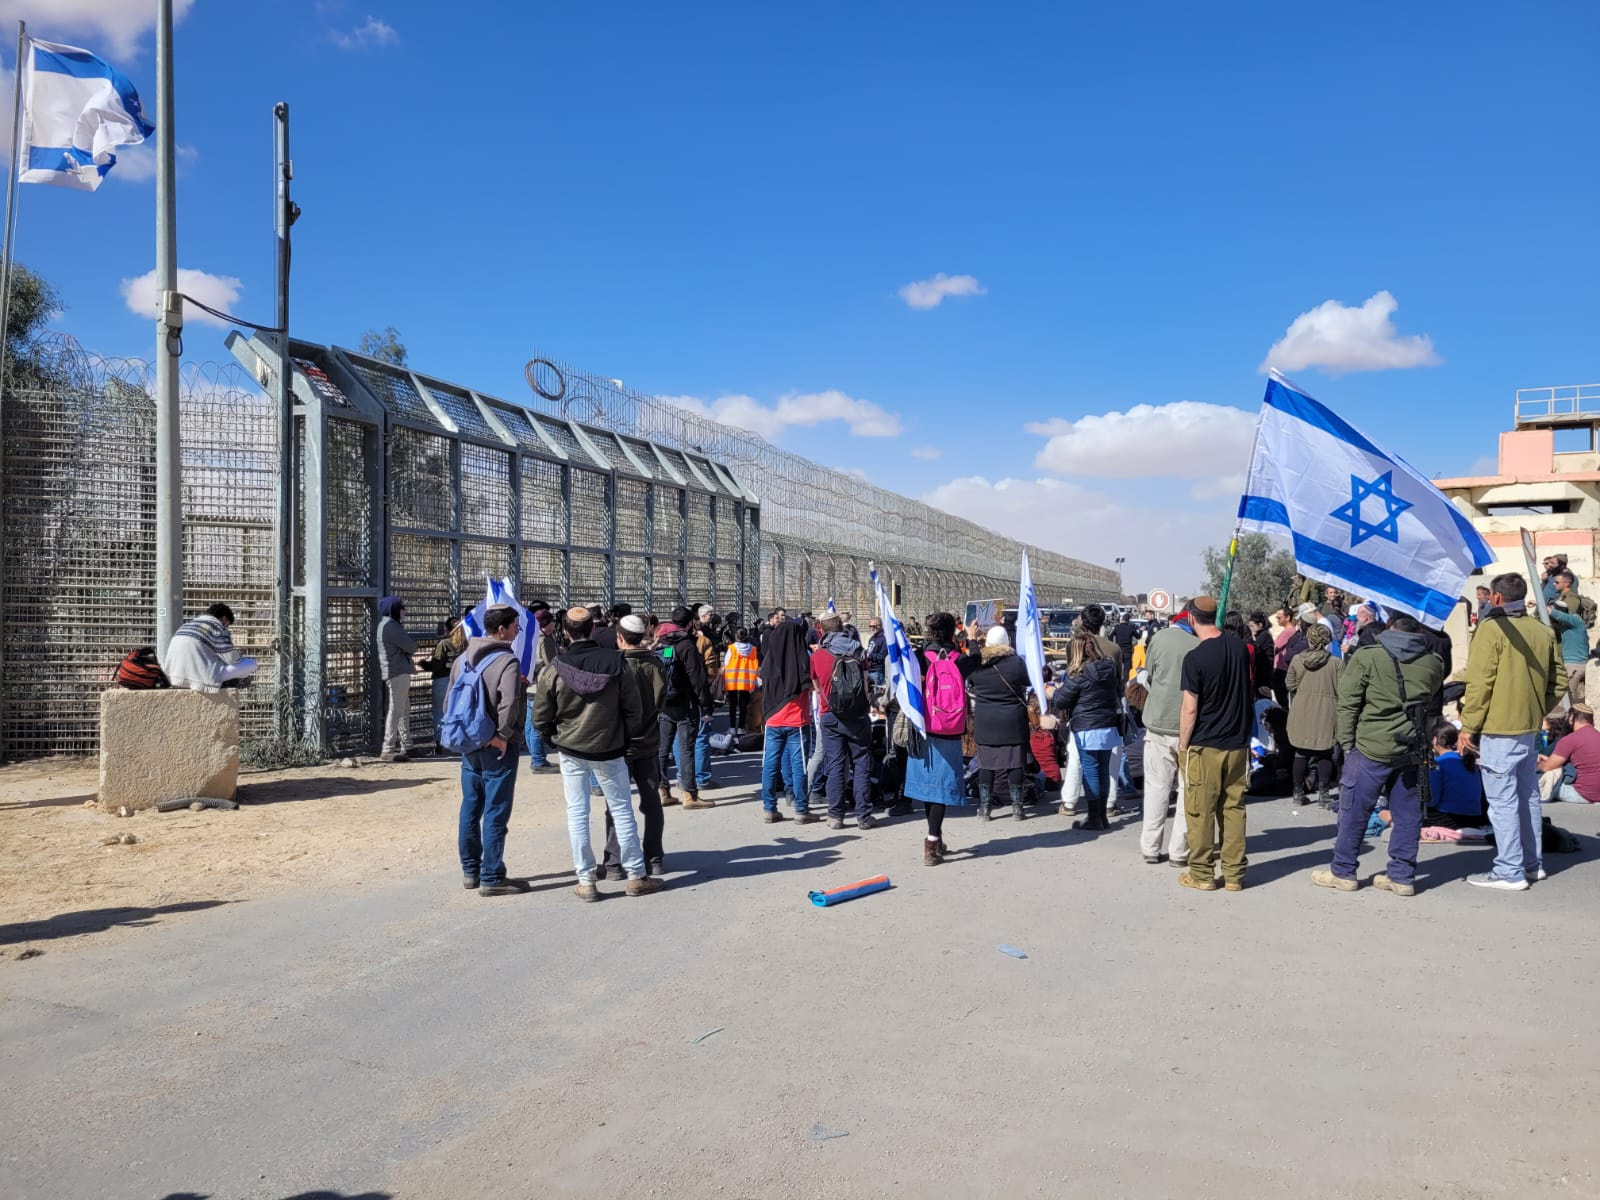
\includegraphics[width=0.85\textwidth]{kerem_shalom_blockade.jpg}
\caption{ফেব্রুয়ারি ২০২৪: ইসরাইলি বিক্ষোভকারীরা কেরেম শালোম ক্রসিংয়ে গাজায় মানবিক ত্রাণ ট্রাক প্রবেশ রোধ করছে। (সূত্র: Wikimedia Commons, CC BY-SA 4.0)}
\end{figure}

\vspace{0.3em}
\noindent{\small\textbf{সূত্র:} Al Jazeera, \textit{Israel Announces Total Blockade on Gaza} (৯ অক্টোবর ২০২৩). \url{https://www.aljazeera.com/news/2023/10/9/israel-announces-total-blockade-on-gaza}; Human Rights Watch, \textit{Gaza: Unlawful Israeli Hospital Attacks Worsen Health Crisis} (নভেম্বর ২০২৩). \url{https://www.hrw.org/news/2023/11/14/gaza-unlawful-israeli-hospital-attacks-worsen-health-crisis}; Wikimedia Commons, \textit{Israelis Blocking Humanitarian Aid Trucks at Kerem Shalom} (ফেব্রুয়ারি ২০২৪, CC BY-SA 4.0). \url{https://commons.wikimedia.org/wiki/File:Hasasat_masaiyot_hasiyua.jpg}}

\subsubsection{খাদ্য উৎপাদন ও সরবরাহ ব্যবস্থার সিস্টেমেটিক
ধ্বংস}\label{ux996ux9a6ux9af-ux989ux9ceux9aaux9a6ux9a8-ux993-ux9b8ux9b0ux9acux9b0ux9b9-ux9acux9afux9acux9b8ux9a5ux9b0-ux9b8ux9b8ux99fux9aeux99fux995-ux9a7ux9acux9b8}

\begin{itemize}
\item
  \textbf{কৃষি জমি ও ফসল ধ্বংস:} গাজার কৃষি উৎপাদন সরঞ্জাম, জমি ও ফসল ধ্বংসের
  ফলে স্থানীয় খাদ্য উৎপাদনের ক্ষমতা ব্যাপকভাবে কমে গেছে। FAO-এর বিশ্লেষণে
  দেখা গেছে গাজার খাদ্য প্রণালীগুলো মারাত্মক ক্ষতিগ্রস্ত হয়েছে এবং খাদ্যের নিজস্ব
  উৎপাদন কমেছে, যা খাদ্য সংকটকে আরও তীব্র করেছে (\emph{FAO \& UNOSAT -
  Question of Palestine}, n.d.)।
\item
  \textbf{খাদ্য গুদাম ও বাজার:} মাঠ পর্যায়ে খাদ্য গুদাম ও বাজারে পরিমাণহীন
  ক্ষতি ও বিরতি ঘটেছে, ফলে খাদ্য সরবরাহের শৃঙ্খল ভেঙেছে এবং বাজারে খাদ্যের
  উপস্থিতি কমে গেছে(\emph{NRC}, 2024)।
\item
  \textbf{মৎস্যজীবন ও প্রোটিন উত্স:} সমুদ্র থেকে মাছ ধরার কার্যক্রম ও
  মৎস্যজীবিদের কার্যক্রমও কঠোরভাবে বাধাপ্রাপ্ত হওয়ায় গাজার প্রাণিজ প্রোটিন উৎসে
  বিরূপ প্রভাব পড়েছে (\emph{english.wafa.ps}, n.d.)।
\end{itemize}

\begin{figure}[h]
\centering
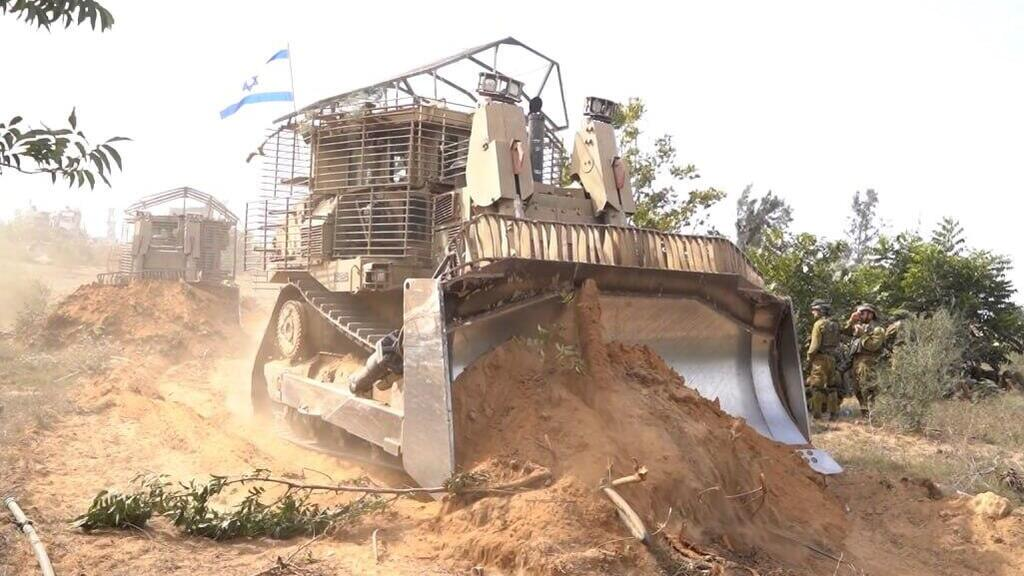
\includegraphics[width=0.82\textwidth]{gaza_bulldozer_farm.jpg}
\caption{অক্টোবর ২০২৩: ইসরাইলি সেনাবাহিনীর ডি-৯আর আর্মড বুলডোজার গাজায় কৃষিজমি ও অবকাঠামো ধ্বংস করছে।
এই পদ্ধতিগত ধ্বংসযজ্ঞে গাজার প্রায় ৬৪--৭০\% বৃক্ষ ফসলের জমি ক্ষতিগ্রস্ত হয়েছে। (সূত্র: IDF Spokesperson, CC BY-SA 4.0)}
\end{figure}

\vspace{0.3em}
\noindent{\small\textbf{সূত্র:} Food and Agriculture Organization (FAO), \textit{Gaza: Geospatial Data Shows Intensifying Damage to Cropland} (২০২৪). \url{https://www.fao.org/neareast/news/details/gaza--geospatial-data-shows-intensifying-damage-to-cropland/en}; Norwegian Refugee Council (NRC), \textit{Food System Collapse in Gaza} (২০২৪). \url{https://www.nrc.no/news/2024/march/food-system-collapse-in-gaza/}}

\subsubsection{জীবন রক্ষাকারী মৌলিক ব্যবস্থার উপর
আঘাত}\label{ux99cux9acux9a8-ux9b0ux995ux9b7ux995ux9b0-ux9aeux9b2ux995-ux9acux9afux9acux9b8ux9a5ux9b0-ux989ux9aaux9b0-ux986ux998ux9a4}

\begin{itemize}
\item
  \textbf{পানি ও স্যানিটেশন:} অবরোধ ও সংঘাতের কারণে পানির বিশুদ্ধতা ও
  সরবরাহ ব্যবস্থা মারাত্মকভাবে ক্ষতিগ্রস্ত হয়েছে। জরুরি পানি সুবিধা প্রায় অপ্রচলিত
  হয়ে পড়েছে (\emph{UN}, 2025)।
\item
  \textbf{বিদ্যুৎ ও জ্বালানি:} গাজার একমাত্র বিদ্যুৎ কেন্দ্রগুলো জ্বালানির অভাবে
  প্রায় বন্ধ হয়ে গেছে, যার প্রভাব হাসপাতাল, পানি শোধনাগার ও স্বাস্থ্য কেন্দ্রসহ
  বিভিন্ন জরুরি পরিষেবায় পড়েছে (\emph{CNN}, 2024)।
\item
  \textbf{স্বাস্থ্য ব্যবস্থা পঙ্গুত্ব:} বিশ্ব স্বাস্থ‌্য সংস্থা (WHO) জানায় যে অনাহার
  পরিস্থিতি ও সহায়তা সীমাবদ্ধতার মধ্যে স্বাস্থ্য কেন্দ্রগুলো কার্যকর সেবা দিতে
  ব্যর্থ হচ্ছে (\emph{UN News}, 2025)।
\end{itemize}

\begin{figure}[h]
\centering
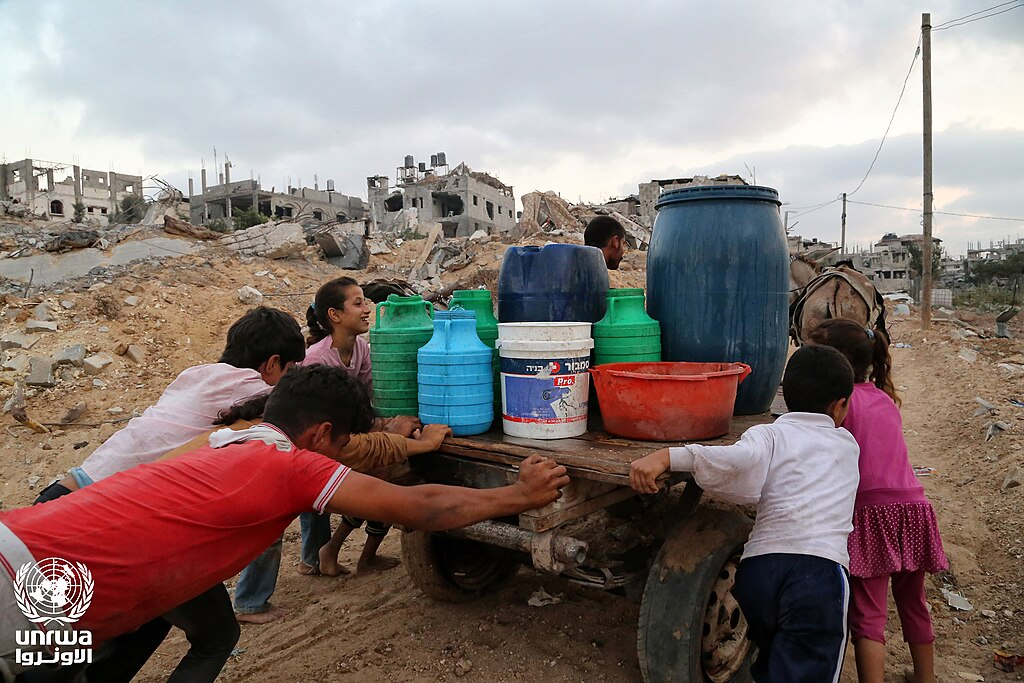
\includegraphics[width=0.82\textwidth]{gaza_water_crisis.jpg}
\caption{গাজায় পানি সংকট তীব্র আকার ধারণ করেছে---প্রতিটি পরিবার মাত্র কয়েক লিটার পানির জন্য মরিয়া হয়ে সংগ্রাম করছে।
ইউএনআরডব্লিউএ-র আলোকচিত্রী ফাদি থাবেতের এই ছবিটি গাজার পানি ও স্বাস্থ্য সংকটের বাস্তব চিত্র তুলে ধরে। (সূত্র: UNRWA/Fadi Thabet, CC BY-SA 3.0 IGO)}
\end{figure}


\vspace{0.3em}
\noindent{\small\textbf{সূত্র:} World Health Organization (WHO), \textit{Gaza Health Cluster Situation Report} (২০২৪). \url{https://www.who.int/news-room/situation-reports/item/situation-report---health-cluster-in-opt-21-september-2024}; UNRWA, \textit{Water Crisis in Gaza} (ফাদি থাবেত, CC BY-SA 3.0 IGO, ২০২৫). \url{https://commons.wikimedia.org/wiki/File:The_water_crisis_in_Gaza_is_severe.jpeg}}

\subsubsection{মানবিক সাহায্য প্রবেশে ইচ্ছাকৃত, নিয়মিত ও মারাত্মক
বাধা}\label{ux9aeux9a8ux9acux995-ux9b8ux9b9ux9afux9af-ux9aaux9b0ux9acux9b6-ux987ux99aux99bux995ux9a4-ux9a8ux9afux9aeux9a4-ux993-ux9aeux9b0ux9a4ux9aeux995-ux9acux9a7}

\begin{itemize}
\item
  \textbf{প্রবেশপথ সীমিতকরণ ও জটিল প্রক্রিয়া:} ত্রাণ প্রবেশের জন্য মাত্র কিছু
  ক্রসিং খোলা থাকে এবং সেখানে কঠোর ও সময়সাপেক্ষ নিরাপত্তা তল্লাশি প্রক্রিয়া
  চালু থাকে, যা দ্রুত সহায়তা পৌঁছাতে বাধা সৃষ্টি করে (\emph{Aid Trucks Queue
  at Rafah Crossing as World Food Day Highlights Gaza's Hunger
  Crisis-Xinhua}, n.d.)।
\item
  \textbf{অনুমোদন ব্যবস্থার জটিলতা:} ত্রাণসম্ভার তালিকায় সরকারি বা প্রশাসনিক
  জটিলতা তৈরির কারণে জরুরি চিকিৎসা সামগ্রী, শিশু খাদ্য ইত্যাদি প্রায়শই আটকে
  থাকে (\emph{Al Jazeera}, 2024)।
\item
  \textbf{ত্রাণ কর্মীদের ওপর বাধা:} ত্রাণকর্মীদের কার্যক্রমে সরাসরি ও পরোক্ষ
  বাধা সৃষ্টি হচ্ছে, যার ফলে সাহায্য বিতরণে খন্ডিততা, বিলম্ব ও মানবিক ক্রমবিলাস
  সৃষ্টি হচ্ছে (\emph{IFJ}, 2026)।
\end{itemize}

\begin{figure}[h]
\centering
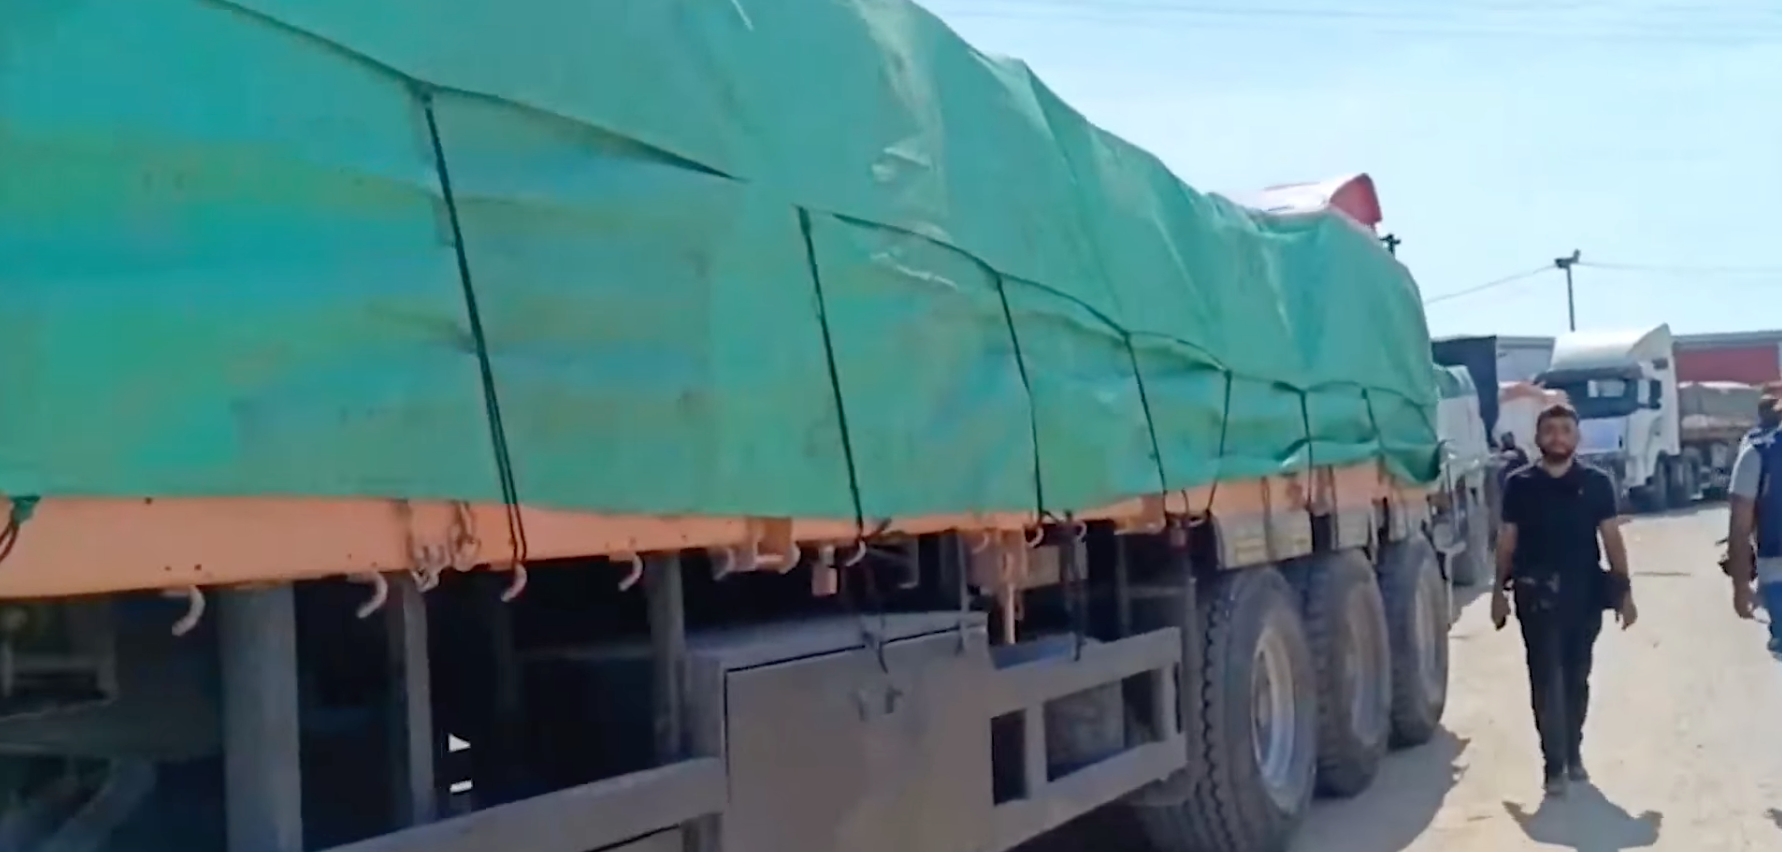
\includegraphics[width=0.82\textwidth]{gaza_aid_blockade.png}
\caption{২০২৩ সালের সম্পূর্ণ অবরোধ ঘোষণার পর গাজার সীমান্তে মানবিক ত্রাণ ট্রাকগুলো প্রবেশের অপেক্ষায় দাঁড়িয়ে আছে।
সামরিক নিয়ন্ত্রণ ও অনুমোদন প্রক্রিয়ার জটিলতায় এই ত্রাণ সামগ্রী মাসের পর মাস বেসামরিক জনগণের কাছে পৌঁছাতে পারেনি। (সূত্র: Tasnim News Agency, CC BY 4.0)}
\end{figure}

\vspace{0.3em}
\noindent{\small\textbf{সূত্র:} UN OCHA, \textit{Gaza Humanitarian Response Update} (মে ২০২৪). \url{https://www.ochaopt.org/content/gaza-humanitarian-response-update-6-12-may-2024}; Al Jazeera, \textit{Aid Trucks Queue at Rafah Crossing as Gaza Hunger Crisis Deepens} (২০২৪). \url{https://www.aljazeera.com/news/2024/10/16/aid-trucks-queue-at-rafah-crossing-as-world-food-day-highlights-gazas}}

\subsection{আন্তর্জাতিক আইনের লঙ্ঘন: একটি স্পষ্ট ও উপেক্ষিত
ফ্রেমওয়ার্ক}\label{ux986ux9a8ux9a4ux9b0ux99cux9a4ux995-ux986ux987ux9a8ux9b0-ux9b2ux999ux998ux9a8-ux98fux995ux99f-ux9b8ux9aaux9b7ux99f-ux993-ux989ux9aaux995ux9b7ux9a4-ux9abux9b0ux9aeux993ux9afux9b0ux995}

২০২৩ সালের অক্টোবরের পর গাজায় ইসরাইলের গৃহীত কৌশলসমূহ---পূর্ণাঙ্গ অবরোধ, খাদ্য
ও পানি সরবরাহ বন্ধ, জীবনরক্ষাকারী অবকাঠামো ধ্বংস এবং মানবিক সহায়তায়
বাধা---আন্তর্জাতিক মানবিক আইন (International Humanitarian Law, IHL) ও
আন্তর্জাতিক মানবাধিকার আইন (International Human Rights Law, IHRL)-এর
একাধিক মৌলিক নীতির সুস্পষ্ট লঙ্ঘন নির্দেশ করে। আন্তর্জাতিক আইন এখানে কেবল নৈতিক
নির্দেশনা নয়; বরং বাধ্যতামূলক আইনি কাঠামো প্রদান করে, যা সংঘাতকালীন
পরিস্থিতিতেও বেসামরিক জনগণের সুরক্ষা নিশ্চিত করে।

\subsubsection{আন্তর্জাতিক মানবিক আইনের (IHL)
লঙ্ঘন}\label{ux986ux9a8ux9a4ux9b0ux99cux9a4ux995-ux9aeux9a8ux9acux995-ux986ux987ux9a8ux9b0-ihl-ux9b2ux999ux998ux9a8}

\begin{itemize}
\item
  \textbf{সমষ্টিগত শাস্তির নিষেধাজ্ঞাঃ} জেনেভা কনভেনশন চতুর্থ (১৯৪৯), অনুচ্ছেদ
  ৩৩ স্পষ্টভাবে ঘোষণা করেঃ ``No protected person may be punished for an
  offence he or she has not personally committed. Collective
  penalties\ldots{} are prohibited.'' গাজায় বসবাসকারী প্রায় ২২ লক্ষ
  বেসামরিক নাগরিককে হামাসের কর্মকাণ্ডের জন্য কার্যত দায়ী করে খাদ্য, পানি,
  বিদ্যুৎ ও চিকিৎসা সরবরাহ থেকে বঞ্চিত করা এই নিষেধাজ্ঞার সরাসরি ও গুরুতর লঙ্ঘন
  (\emph{IHL Treaties - Geneva Convention (IV) on Civilians, 1949 -
  Article 33}, n.d.)।
\item
  \textbf{বেসামরিক জনগণের জন্য অপরিহার্য বস্তুর সুরক্ষাঃ} জেনেভা কনভেনশনসমূহের
  অতিরিক্ত প্রোটোকল I (১৯৭৭), অনুচ্ছেদ ৫৪ ঘোষণা করেঃ ``Starvation of
  civilians as a method of warfare is prohibited.'' এবং আরও স্পষ্টভাবে বলা
  হয়েছে যে খাদ্য, কৃষি এলাকা, ফসল, পশুসম্পদ, পানীয় জলের সরবরাহ ও সেচব্যবস্থা
  ধ্বংস বা অকেজো করা নিষিদ্ধ। গাজায় কৃষিজমি ধ্বংস, খাদ্য গুদাম লক্ষ্যবস্তু করা,
  পানি ও স্যানিটেশন ব্যবস্থা অকার্যকর করা এই অনুচ্ছেদের প্রতিটি উপাদানের লঙ্ঘন
  নির্দেশ করে (\emph{IHL Treaties - Additional Protocol (I) to the Geneva
  Conventions, 1977 - Article 54}, n.d.)।
\end{itemize}

\subsubsection{আন্তর্জাতিক মানবাধিকার আইনের (IHRL)
লঙ্ঘন}\label{ux986ux9a8ux9a4ux9b0ux99cux9a4ux995-ux9aeux9a8ux9acux9a7ux995ux9b0-ux986ux987ux9a8ux9b0-ihrl-ux9b2ux999ux998ux9a8}

সংঘাতকালীন পরিস্থিতিতেও মানবাধিকার আইন সম্পূর্ণভাবে স্থগিত হয় না। অর্থনৈতিক,
সামাজিক ও সাংস্কৃতিক অধিকার সংক্রান্ত আন্তর্জাতিক চুক্তি (ICESCR) অনুযায়ী:

\begin{itemize}
\item
  খাদ্যের অধিকার (Article 11)
\item
  স্বাস্থ্যের সর্বোচ্চ অর্জনযোগ্য মানের অধিকার (Article 12)
\item
  নিরাপদ পানীয় জলের অধিকার (General Comment No. 15)
\end{itemize}

গাজায় খাদ্য, পানি, স্বাস্থ্যসেবা ও ওষুধের প্রবেশে বাধা এই অধিকারগুলোর চরম লঙ্ঘন।
জাতিসংঘের বিভিন্ন বিশেষ র‌্যাপোর্টিয়ার এই পরিস্থিতিকে ``man-made humanitarian
catastrophe'' হিসেবে আখ্যায়িত করেছেন \emph{OHCHR}, n.d.)।

\subsubsection{\texorpdfstring{৩.৪.৩ ইসরাইলের ``সুরক্ষা অজুহাত'' ও
``মানবঢাল যুক্তি''-র আইনি খণ্ডন
}{৩.৪.৩ ইসরাইলের ``সুরক্ষা অজুহাত'' ও ``মানবঢাল যুক্তি''-র আইনি খণ্ডন }}\label{ux987ux9b8ux9b0ux987ux9b2ux9b0-ux9b8ux9b0ux995ux9b7-ux985ux99cux9b9ux9a4-ux993-ux9aeux9a8ux9acux9a2ux9b2-ux9afux995ux9a4-ux9b0-ux986ux987ux9a8-ux996ux9a3ux9a1ux9a8}

ইসরাইল তার কর্মকাণ্ডের বৈধতা দেয় দুই যুক্তিতে।~প্রথমত\textbf{,} তারা দাবি করে
অবরোধ হামাসের সামরিক সক্ষমতা দুর্বল করতে ``প্রয়োজনীয়''।~দ্বিতীয়ত, তারা
হামাসের বেসামরিক স্থাপনা ব্যবহারকে জীবনরক্ষাকারী অবকাঠামো ধ্বংসের কারণ
হিসেবে উল্লেখ করে। আন্তর্জাতিক মানবিক আইনের দৃষ্টিতে এই যুক্তিগুলো অগ্রহণযোগ্য।

এর খণ্ডন নিম্নরূপ:~আইনের আনুপাতিকতা (Proportionality) ও বৈষম্য (Distinction)
নীতির আলোকে~একটি বৈধ সামরিক লক্ষ্য (হামাসকে দুর্বল করা) অর্জনের জন্য
গাজার~সমগ্র বেসামরিক জনগোষ্ঠীকে~খাদ্য, পানি, বিদ্যুৎ ও চিকিৎসা থেকে বঞ্চিত করা
কোনোভাবেই~আনুপাতিক নয়। এটি আইনের সুস্পষ্ট লঙ্ঘন এবং একটি~সমষ্টিগত শাস্তি, যা
জেনেভা কনভেনশন চতুর্থের অনুচ্ছেদ ৩৩ দ্বারা সম্পূর্ণ নিষিদ্ধ। এছাড়া,~দখলদার শক্তি
(Occupying Power)~হিসেবে ইসরাইলের দায়িত্ব হামাসের আচরণ দ্বারা লোপ পায়
না।~জেনেভা কনভেনশন চতুর্থের অনুচ্ছেদ ৫৫ ও ৫৬~ইসরাইলকে বাধ্য করে অধিকৃত ভূখণ্ডের
জনগণের~খাদ্য ও চিকিৎসা সরবরাহ নিশ্চিত করতে\textbf{~}এবং~জনস্বাস্থ্য ও
হাসপাতাল ব্যবস্থা বজায় রাখতে। ফলে, প্রতিপক্ষের কর্মকাণ্ডের অজুহাতে জীবন
রক্ষাকারী অবকাঠামোর রক্ষণাবেক্ষণ ও সরবরাহ থেকে সরে আসা আইনত বৈধ নয়
(\emph{IHL Treaties - Geneva Convention (IV) on Civilians, 1949},
n.d.-b)।

\subsection{\texorpdfstring{অভিপ্রায় ও প্রমাণ বিশ্লেষণ
}{৩.৫ অভিপ্রায় ও প্রমাণ বিশ্লেষণ }}\label{ux985ux9adux9aaux9b0ux9df-ux993-ux9aaux9b0ux9aeux9a3-ux9acux9b6ux9b2ux9b7ux9a3}

আন্তর্জাতিক মানবিক আইন (IHL) ও আন্তর্জাতিক অপরাধ আইনের (ICC) ক্ষেত্রে কোনো
আচরণকে যুদ্ধাপরাধ বা গুরুতর আইনি লঙ্ঘন হিসাবে ঘোষণা করার জন্য শুধু ফলাফল নয়,
অভিপ্রায় (intent) নিরূপণ গুরুত্বপূর্ণ ভূমিকা পালন করে। বিশেষত অনাহারকে যুদ্ধাস্ত্র
হিসেবে ব্যবহারের ক্ষেত্রে আন্তর্জাতিক নীতিমালা স্পষ্টভাবে ইচ্ছাকৃত সিদ্ধান্ত ও
আচরণকে গুরুত্ব দেয়।

~নিম্নলিখিত প্রমাণের সামগ্রিকতা (Totality of Circumstances) থেকে আদালত
অভিপ্রায় অনুমান করে:

\begin{itemize}
\item
  \textbf{প্রকাশ্য বিবৃতি ও ঘোষণা:}~২০২৩ সালের ৯ অক্টোবর ইসরাইলি
  প্রতিরক্ষামন্ত্রীর ``বিদ্যুৎ, খাবার, পানি, গ্যাস---সবকিছু বন্ধ করে দেওয়া হবে''
  ঘোষণা আন্তর্জাতিক আইনের আলোকে অত্যন্ত তাৎপর্যপূর্ণ। এই ধরনের স্পষ্ট ও বিস্তৃত
  ঘোষণা কেবল একটি সামরিক কৌশল নয়, বরং বেসামরিক জনগণের জীবনধারণের উপকরণকে
  লক্ষ্যবস্তু করার একটি নীতিগত অবস্থান নির্দেশ করে।
\end{itemize}

\begin{quote}
এ ধরনের বক্তব্য আন্তর্জাতিক বিচারিক অনুশীলনে (jurisprudence) গুরুত্বপূর্ণ প্রমাণ
হিসেবে বিবেচিত হয়েছে। উদাহরণস্বরূপ, Bosnian War চলাকালে বিভিন্ন সামরিক ও
রাজনৈতিক নেতাদের প্রকাশ্য বক্তব্য পরবর্তীতে তাদের অভিপ্রায় নির্ধারণে গুরুত্বপূর্ণ
ভূমিকা পালন করে, বিশেষত Siege of Sarajevo-এর সময় বেসামরিক জনগণের ওপর চাপ
সৃষ্টি করার কৌশল বিশ্লেষণে।
\end{quote}

\begin{itemize}
\item
  \textbf{পরিকল্পিত নীতির ধারাবাহিকতা:}~একক বা বিচ্ছিন্ন ঘটনার পরিবর্তে, যদি
  একাধিক কর্মকাণ্ড একটি ধারাবাহিক কৌশলগত প্যাটার্ন নির্দেশ করে, তবে তা
  অভিপ্রায় নিরূপণে শক্তিশালী প্রমাণ হিসেবে বিবেচিত হয়। গাজার ক্ষেত্রে
  নিম্নলিখিত পদক্ষেপগুলো একটি সুসংগঠিত নীতির ইঙ্গিত দেয়:
\end{itemize}

\begin{itemize}
\item
  দীর্ঘমেয়াদি অবরোধ ও পণ্য প্রবেশে কঠোর নিয়ন্ত্রণ
\item
  কৃষিজমি, খাদ্য গুদাম এবং উৎপাদন অবকাঠামো ধ্বংস
\item
  পানি সরবরাহ ব্যবস্থা ও বিদ্যুৎ অবকাঠামোর ওপর আঘাত
\item
  জ্বালানি সরবরাহ সীমিত বা বন্ধ করা
\item
  মানবিক সহায়তা প্রবেশে প্রশাসনিক ও লজিস্টিক বাধা সৃষ্টি
\end{itemize}

\begin{quote}
এই ধারাবাহিক কর্মকাণ্ডগুলো কেবল সামরিক লক্ষ্য অর্জনের জন্য নয়, বরং বেসামরিক
জনগণের জীবনধারণের সক্ষমতাকে পদ্ধতিগতভাবে দুর্বল করার একটি সুস্পষ্ট কৌশল নির্দেশ
করে। তুলনামূলকভাবে, Yemen Civil War-এ অবরোধ ও খাদ্য সরবরাহে বাধা সৃষ্টির
মাধ্যমে অনাহার পরিস্থিতি তৈরির অভিযোগ আন্তর্জাতিক মহলে একই ধরনের আইনি
বিতর্কের জন্ম দিয়েছে।
\end{quote}

\begin{itemize}
\item
  \textbf{পরিণামের পূর্বজ্ঞান:}~আন্তর্জাতিক আইনে একটি গুরুত্বপূর্ণ নীতি হলো---যদি
  কোনো কর্মকাণ্ডের স্বাভাবিক ও অনিবার্য ফলাফল গুরুতর ক্ষতি (যেমন অনাহার) হয় এবং
  সেই ফলাফল সম্পর্কে সংশ্লিষ্ট পক্ষ পূর্বেই অবগত থাকে, তবে সেই কর্মকাণ্ডকে ইচ্ছাকৃত
  হিসেবে বিবেচনা করা যেতে পারে।
\end{itemize}

\begin{quote}
গাজার ক্ষেত্রে, অবরোধ, খাদ্য সরবরাহে বাধা এবং অবকাঠামো ধ্বংসের ফলে অনাহার,
অপুষ্টি এবং মানবিক বিপর্যয় ঘটবে---এটি একটি সুপরিচিত ও পূর্বানুমেয় ফলাফল। World
Food Programme এবং Food and Agriculture Organization দীর্ঘদিন ধরে সতর্ক
করে আসছে যে, এই ধরনের অবরোধ খাদ্য নিরাপত্তাহীনতাকে তীব্র করে তোলে এবং
দুর্ভিক্ষের ঝুঁকি বাড়ায়। তা সত্ত্বেও যদি একই ধরনের নীতি অব্যাহত থাকে, তবে তা
অভিপ্রায় নির্দেশ করে।
\end{quote}

\begin{itemize}
\item
  \textbf{আইনি প্রেক্ষাপট:}~জেনেভা কনভেনশন এর অধীনে, বিশেষত অনুচ্ছেদ ৫৫ ও ৫৬
  অনুযায়ী, দখলদার শক্তির ওপর বেসামরিক জনগণের খাদ্য, চিকিৎসা ও জনস্বাস্থ্য
  নিশ্চিত করার দায়িত্ব বর্তায়। এই দায়িত্ব কেবল নেতিবাচক (ক্ষতি না করা) নয়,
  বরং ইতিবাচক (প্রয়োজনীয় সরবরাহ নিশ্চিত করা)। যদি কোনো রাষ্ট্র সচেতনভাবে এই
  দায়িত্ব পালন করতে ব্যর্থ হয় বা বাধা সৃষ্টি করে, তবে তা কেবল অবহেলা নয়, বরং
  ইচ্ছাকৃত উপেক্ষা (wilful neglect) হিসেবে বিবেচিত হতে পারে। উদাহরণস্বরূপ,
  Nuremberg Trials-এ মানবিক দায়িত্ব লঙ্ঘনের ক্ষেত্রে পরিকল্পিত অবহেলাকে
  অপরাধমূলক অভিপ্রায়ের অংশ হিসেবে গণ্য করা হয়েছিল।
\end{itemize}

উপরোক্ত সব উপাদান---(ক) প্রকাশ্য ঘোষণা, (খ) ধারাবাহিক ও পদ্ধতিগত কর্মকৌশল,
(গ) পরিণামের পূর্বজ্ঞান, এবং (ঘ) আইনি দায়িত্বের সচেতন উপেক্ষা---একত্রে একটি
শক্তিশালী প্রমাণভিত্তিক কাঠামো তৈরি করে। আন্তর্জাতিক ফৌজদারি আইনে এই ধরনের
সমন্বিত বিশ্লেষণ (cumulative approach) অভিপ্রায় নির্ধারণে অত্যন্ত গুরুত্বপূর্ণ।
গাজার প্রেক্ষাপটে এই প্রমাণসমূহ সম্মিলিতভাবে নির্দেশ করে যে, বেসামরিক জনগণের
অনাহার ও দুর্ভোগকে কেবল যুদ্ধের অনিবার্য পার্শ্বপ্রতিক্রিয়া হিসেবে ব্যাখ্যা করা
কঠিন। বরং এটি একটি পূর্বপরিকল্পিত, কাঠামোগত ও ধারাবাহিক নীতির ফলাফল হিসেবে
প্রতীয়মান হয়, যা আন্তর্জাতিক আইনের আলোকে গুরুতর প্রশ্ন উত্থাপন করে।

\section{\texorpdfstring{৪র্থ অধ্যায়: প্রভাব ও ফলাফল}{৪র্থ অধ্যায়: প্রভাব ও ফলাফল}}\label{ux9a5ux9b0-ux985ux9a7ux9afux9df-ux9aaux9b0ux9adux9ac-ux993-ux9abux9b2ux9abux9b2}

\subsection{ভূমিকা}\label{ux9adux9aeux995-2}

২০২৩-২০২৪ সালের গাজা যুদ্ধে ইসরাইলের কৌশলগত অবরোধ ও জীবন-জীবিকা ধ্বংসের
পদক্ষেপসমূহ গাজার ২২ লক্ষ বেসামরিক নাগরিকের উপর এক গভীর ও বহুমুখী মানবিক সংকট
তৈরি করেছে। এই অধ্যায়ে অনাহার-কৌশলের ফলে সৃষ্ট সামগ্রিক প্রভাব ও ফলাফলকে
কাঠামোগতভাবে বিশ্লেষণ করা হবে। আলোচনা করা হবে খাদ্য নিরাপত্তাহীনতা, স্বাস্থ্য
ব্যবস্থার পতন, শিশু ও নারীদের উপর বিশেষ প্রভাব, দীর্ঘমেয়াদী সামাজিক ও মানসিক
ট্রমা, এবং ভবিষ্যৎ প্রজন্মের সম্ভাবনার ধ্বংস সম্পর্কে।

\subsection{\texorpdfstring{খাদ্য নিরাপত্তাহীনতা ও দুর্ভিক্ষ-সদৃশ পরিস্থিতি
}{৪.২ খাদ্য নিরাপত্তাহীনতা ও দুর্ভিক্ষ-সদৃশ পরিস্থিতি }}\label{ux996ux9a6ux9af-ux9a8ux9b0ux9aaux9a4ux9a4ux9b9ux9a8ux9a4-ux993-ux9a6ux9b0ux9adux995ux9b7-ux9b8ux9a6ux9b6-ux9aaux9b0ux9b8ux9a5ux9a4}

\subsubsection{\texorpdfstring{৪.২.১ পরিসংখ্যানগত চিত্র
}{৪.২.১ পরিসংখ্যানগত চিত্র }}\label{ux9aaux9b0ux9b8ux996ux9afux9a8ux997ux9a4-ux99aux9a4ux9b0}

\begin{itemize}
\item
  ২০২৪ সালের সেপ্টেম্বর-অক্টোবরে গাজার পুরো ভূখণ্ড IPC ফেজ ৪ (জরুরি অবস্থা)-এ
  রয়েছে। গাজায় ১৮ লক্ষ ৪০ হাজার মানুষ তীব্র খাদ্য নিরাপত্তাহীনতায় ভুগছে (IPC
  ফেজ ৩ বা তার উপরে। এর মধ্যে ১ লক্ষ ৩৩ হাজার মানুষ বিপর্যয়কর খাদ্য
  নিরাপত্তাহীনতায় (IPC ফেজ ৫) এবং ৬ লক্ষ ৬৪ হাজার মানুষ জরুরি অবস্থায় (IPC
  ফেজ ৪) রয়েছে। শত্রুতার বৃদ্ধির আগের সময়ের তুলনায় তীব্র অপুষ্টির হার দশ গুণ বৃদ্ধি
  পেয়েছে (\emph{IPC Special Snapshot - September 2024 - April 2025)}।
\item
  \textbf{শিশু অপুষ্টি}: ৫ বছরের কম বয়সী শিশুদের ৩০\% মারাত্মক অপুষ্টিতে
  আক্রান্ত, যা জীবন-হুমকির অবস্থা সৃষ্টি করেছে (\emph{More than 5,000 Children
  Diagnosed with Malnutrition in the Gaza Strip in May},2925)।
\item
  \textbf{খাদ্য মূল্য বৃদ্ধি}: অবরোধ ও সরবরাহ বন্ধের কারণে গাজায় খাদ্যপণ্যের দাম
  ৩০০\%-৮০০\% পর্যন্ত বৃদ্ধি পেয়েছে (\emph{GAZA / FOOD PRICES AND SCARCITY
  \textbar{} UNifeed}, n.d.)।
\end{itemize}

\subsection{শিশু, নারী ও বিশেষ ঝুঁকিপূর্ণ জনগোষ্ঠীর উপর
প্রভাব}\label{ux9b6ux9b6-ux9a8ux9b0-ux993-ux9acux9b6ux9b7-ux99dux995ux9aaux9b0ux9a3-ux99cux9a8ux997ux9b7ux9a0ux9b0-ux989ux9aaux9b0-ux9aaux9b0ux9adux9ac}

\subsubsection{\texorpdfstring{৪.৩.১ শিশুদের উপর প্রভাব
}{৪.৩.১ শিশুদের উপর প্রভাব }}\label{ux9b6ux9b6ux9a6ux9b0-ux989ux9aaux9b0-ux9aaux9b0ux9adux9ac}


\begin{figure}[h]
\centering
\begin{minipage}{0.48\textwidth}
\centering
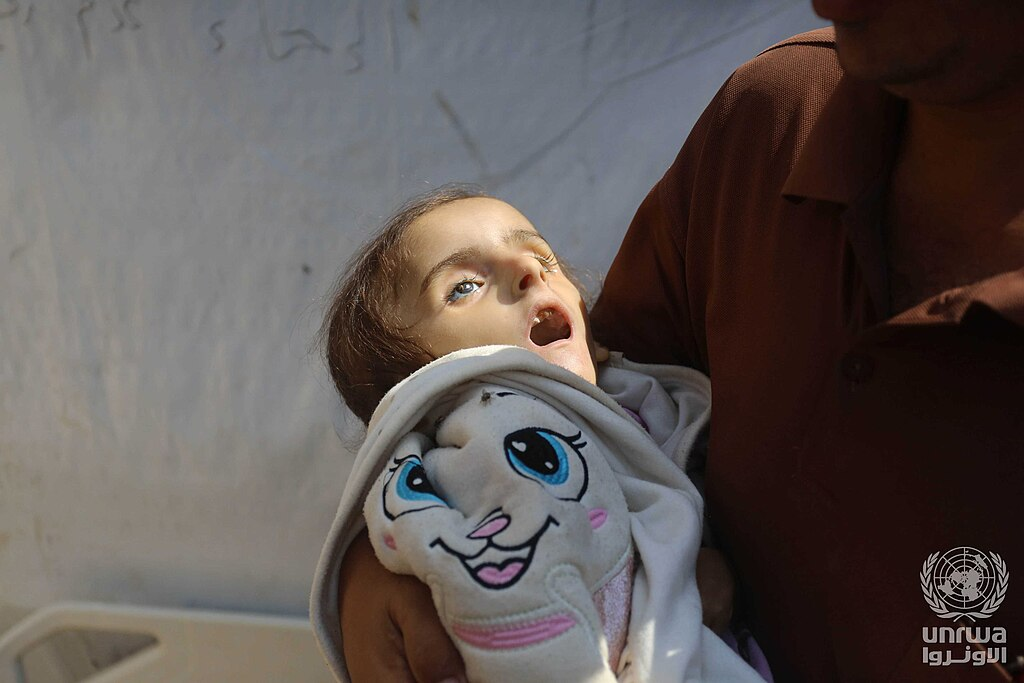
\includegraphics[width=\linewidth]{gaza_child_malnutrition.jpg}
\end{minipage}
\hfill
\begin{minipage}{0.48\textwidth}
\centering
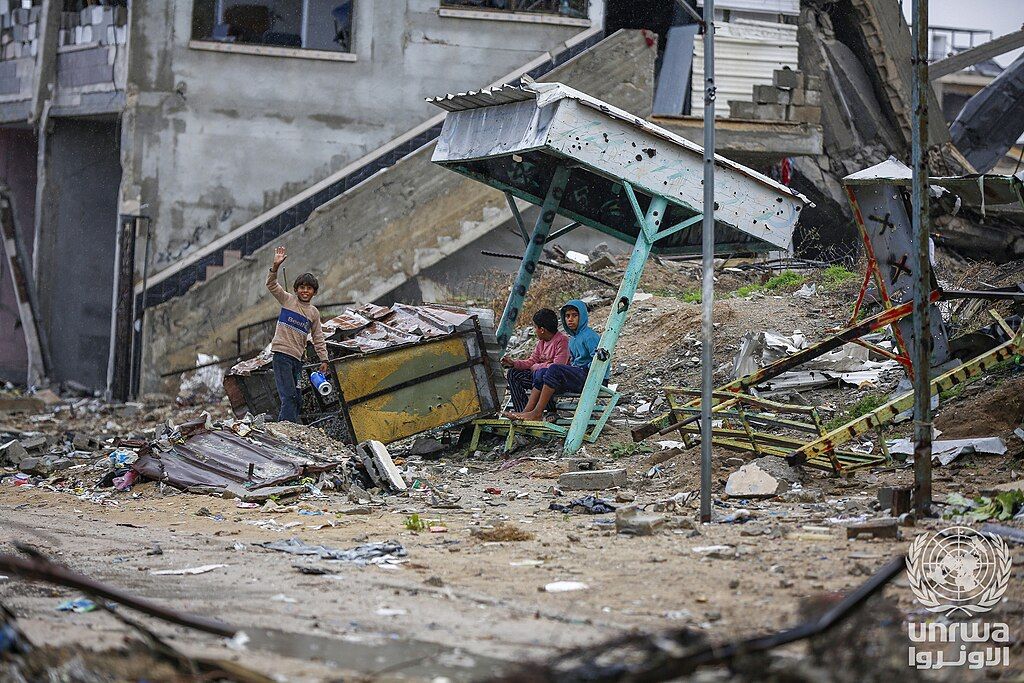
\includegraphics[width=\linewidth]{gaza_children_displaced.jpg}
\end{minipage}
\caption{\textbf{বাম:} আগস্ট ২০২৪ — অপুষ্টি ও চিকিৎসার অভাবে মৃত্যুবরণকারী ৪ বছর বয়সী ফিলিস্তিনি শিশু। \textbf{ডান:} জানুয়ারি ২০২৫ — নুসাইরাত শরণার্থী শিবিরে ধ্বংসস্তূপের উপর বসা বাস্তুচ্যুত শিশুরা। (সূত্র: UNRWA/Ashraf Amra, CC BY-SA 3.0 IGO)}
\end{figure}

\vspace{0.3em}
\noindent{\small\textbf{সূত্র:} UNRWA/Ashraf Amra, \textit{A 4-Year-Old Palestinian Girl Lost Her Life Due to Malnutrition} (আগস্ট ২০২৪, CC BY-SA 3.0 IGO). \url{https://commons.wikimedia.org/wiki/File:A_4-year-old_Palestinian_girl,_lost_her_life_due_to_malnutrition_and_lack_of_treatment_due_to_the_war_on_Gaza.jpg}; UNRWA/Ashraf Amra, \textit{Displaced Children on Rubble in Nuseirat Camp} (জানুয়ারি ২০২৫, CC BY-SA 3.0 IGO). \url{https://commons.wikimedia.org/wiki/File:Displaced_children_sit_on_the_rubble_of_their_destroyed_home_in_Nuseirat_camp,_Gaza_Strip.jpg}}

গাজার শিশুদের ওপর অনাহার-কৌশলের প্রভাব অত্যন্ত গভীর ও বহুমাত্রিক, যেখানে
শারীরিক, মানসিক ও শিক্ষাগত ক্ষেত্রগুলোই একসাথে ক্ষতিগ্রস্ত হচ্ছে; খাদ্য নিরাপত্তা
ভেঙে পড়ায় ২০২৫ সালের মে মাসে ৫,১১৯ জন ৬ মাস থেকে ৫ বছর বয়সী শিশু তীব্র
অপুষ্টিতে ভর্তি হয়েছে, যাদের মধ্যে ৬৩৬ জনের অবস্থাকে সিভিয়ার অ্যাকিউট
মালনিউট্রিশন (SAM) হিসেবে চিহ্নিত করা হয়েছে, যা পুনর্বাসনের জন্য ধারাবাহিক
চিকিৎসা, নিরাপদ পানি ও পুষ্টিগত সহায়তা ছাড়াই জীবন-হুমকিস্বরূপ হয়। এই শারীরিক
নির্ভেজাল ক্ষতির পাশাপাশি, যুদ্ধের ভয়াবহ পরিবেশে শিশুরা মানসিক ট্রমা, PTSD,
দুশ্চিন্তা ও বিষণ্নতায় ভুগছে, যা তাদের স্নায়বিক ও আবেগীয় বিকাশকে দীর্ঘমেয়াদে
বাধাগ্রস্ত করে এবং সামাজিক সহায়তা ব্যবস্থা ভেঙে পড়ার ফলে তারা নিরাপদ পরিবেশ
বা সহায়তা পায় না। এছাড়া, অবরুদ্ধ অবস্থায় স্কুল ও শিক্ষাপ্রতিষ্ঠানগুলো ধ্বংস ও
নিরাপত্তাহীনতার কারণে বন্ধ থাকায় শিশুরা শিক্ষা থেকে বঞ্চিত হচ্ছে, যা তাদের
শিখনক্ষমতা ও ভবিষ্যৎ সম্ভাবনায় দীর্ঘমেয়াদি নেতিবাচক প্রভাব ফেলছে, ফলে একটি
সম্পূর্ণ প্রজন্ম শিক্ষাগত ও স্বাস্থ্যগতভাবে ক্ষতিগ্রস্ত হওয়ার ঝুঁকিতে রয়েছে
(\emph{More than 5,000 Children Diagnosed with Malnutrition in the Gaza
Strip in May}, n.d.-b)।

\subsubsection{\texorpdfstring{৪.৩.২ নারী ও মাতৃস্বাস্থ্যের উপর প্রভাব
}{৪.৩.২ নারী ও মাতৃস্বাস্থ্যের উপর প্রভাব }}\label{ux9a8ux9b0-ux993-ux9aeux9a4ux9b8ux9acux9b8ux9a5ux9afux9b0-ux989ux9aaux9b0-ux9aaux9b0ux9adux9ac}

\begin{figure}[h]
\centering
\begin{minipage}{0.48\textwidth}
\centering
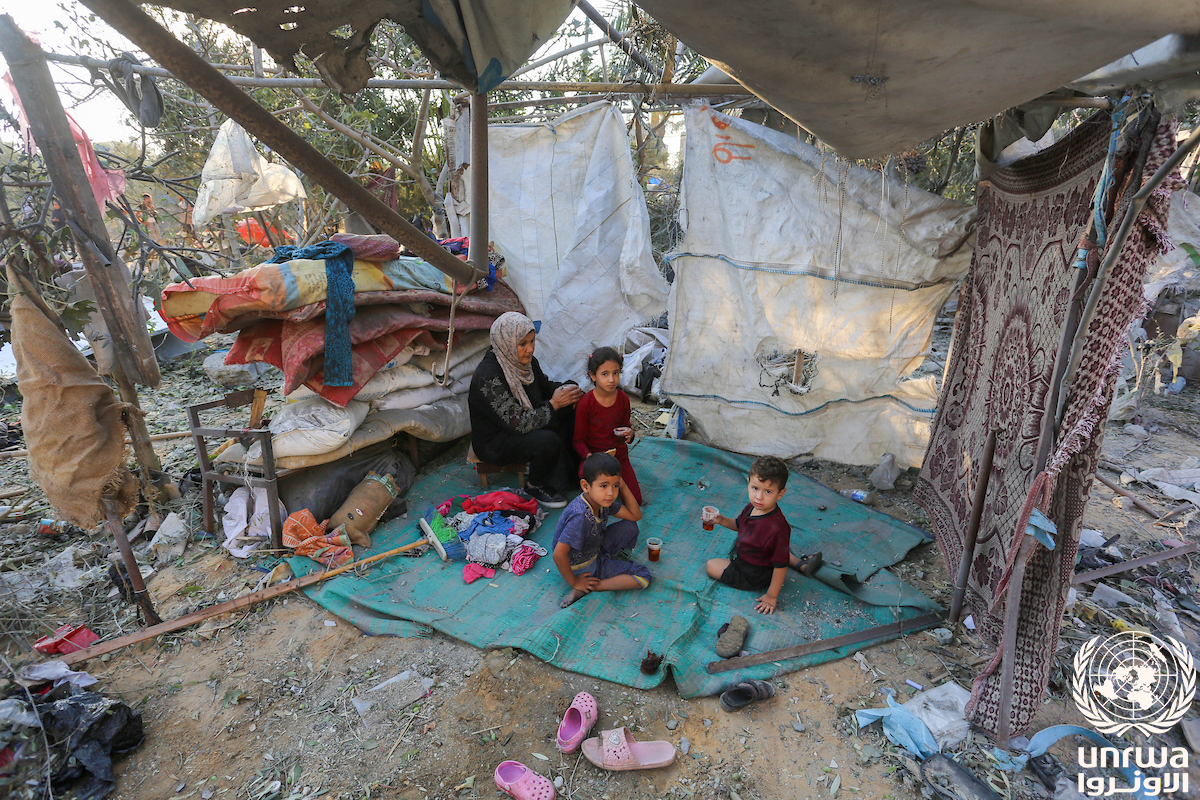
\includegraphics[width=\linewidth]{gaza_woman_children.jpg}
\end{minipage}
\hfill
\begin{minipage}{0.48\textwidth}
\centering
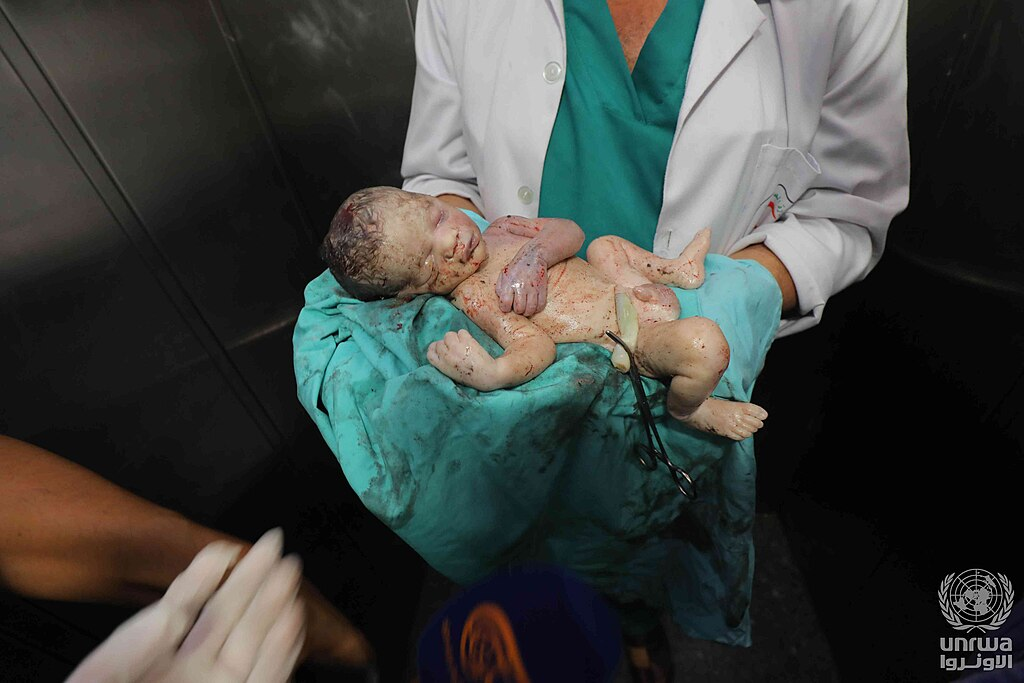
\includegraphics[width=\linewidth]{gaza_newborn_killed.jpg}
\end{minipage}
\caption{\textbf{বাম:} আগস্ট ২০২৪ — ইসরাইলি বিমান হামলায় ধ্বংসস্তূপের সামনে বসে থাকা একজন ফিলিস্তিনি মা তার সন্তানদের নিয়ে, দেইর আল-বালাহ, গাজা। \textbf{ডান:} অক্টোবর ২০২৩ — নুসাইরাত শরণার্থী শিবিরে ইসরাইলি বিমান হামলায় নিহত নবজাতক শিশু। (সূত্র: UNRWA/Ashraf Amra, CC BY-SA 3.0 IGO)}
\end{figure}
\vspace{0.3em}
\noindent{\small\textbf{সূত্র:} UNRWA/Ashraf Amra, \textit{Palestinian woman with children in front of destroyed home, Deir el-Balah} (August 7, 2024) \& \textit{Newborn baby killed in Israeli airstrike of Nuseirat camp} (October 31, 2023). Wikimedia Commons, CC BY-SA 3.0 IGO. \url{https://creativecommons.org/licenses/by-sa/3.0/igo/}}

গাজায় অনাহার ও খাদ্য নিরাপত্তার ধসের ফলে গর্ভবতী ও স্তন্যদানকারী মায়েদের ওপর
মারাত্মক বিপজ্জনক পরিস্থিতি সৃষ্টি হয়েছে। খাদ্যের অভাবে মায়ের শরীর পর্যাপ্ত পুষ্টি
না পাওয়ায় গর্ভকালীন জটিলতা, গর্ভপাত, মৃতপ্রসব ও কম ওজনের শিশু জন্মের হার
উল্লেখযোগ্যভাবে বৃদ্ধি পেয়েছে। অনাহার শুধু শারীরিক ক্ষতি নয়; এটি সরাসরি সন্তান ও
মাতৃস্বাস্থ্যের জন্য জীবন-হুমকিস্বরূপ হয়ে দাঁড়িয়েছে। UNFPA বলেছে, বহু মারাত্মক
ক্ষেত্রে মায়েরা ``খাদ্য, পানীয় ও পুষ্টি না পেয়ে ক্লান্ত, দুর্বল ও মৃত্যুর ঝুঁকিতে''
জন্ম দিতে বাধ্য হচ্ছেন, যার ফলে তাদের শিশুরা শক্তি-হীন, কম ওজন বা প্রিম্যাচিউর
(সময় থেকে আগেই) জন্মগ্রহণ করছে এবং অনেকসময় দেখা যাচ্ছে মা নিজের অক্ষমতার
কারণে স্তনপান করাতে পারছেন না। UNFPA-এর মূল্যায়ন অনুযায়ী, গাজার প্রায় ৪০\%
গর্ভবতী ও স্তন্যদানকারী মায়েরা তীব্র অপুষ্টিতে ভুগছেন এবং আনুমানিক ৫৫,০০০ এর
বেশি গর্ভবতী ও স্তন্যদানকারী নারী ২০২৬ সালের মধ্যভাগে মারাত্মকভাবে ক্ষতিগ্রস্ত
হতে পারেন, যেখানে অনেক শিশু সময়ে আগেই জন্ম নিচ্ছেন বা খুব কম ওজন নিয়ে জন্ম
নিচ্ছেন, যা তাদের বাঁচার সম্ভাবনাকেও কমিয়ে দেয়। (\emph{United Nations
Population Fund}, n.d.)

স্বাস্থ্যব্যবস্থার অবনতি এই ঝুঁকি আরও বাড়িয়ে দিয়েছে। চিকিৎসা কেন্দ্রগুলোর জ্বালানি
ও ওষুধের অভাবে প্রয়োজনীয় চিকিৎসা সেবা প্রদান অসম্পূর্ণ---অনেক ক্ষেত্রে গর্ভাবস্থায়
জটিলতা, অস্ত্রোপচার বা জরুরি সেবা \emph{অ্যানেস্থেশিয়া বা পর্যাপ্ত ওষুধ ছাড়া}
করতে হচ্ছে, যা মায়ের জীবনকে সরাসরি ঝুঁকির মুখে ফেলে। এই পরিস্থিতিতে,
\emph{গর্ভকালীন ও প্রসূতি সেবা প্রায় সংকুচিত অবস্থায়}, বিশেষত হাসপাতালগুলো যখন
বিদ্যুতের অভাবে কার্যত অচল বা সীমিত সেবা দিচ্ছে (\emph{UNFPA} n.d.)।

এছাড়া, অপুষ্টি ও স্বাস্থ্যসেবা সংকটের মিলিত প্রভাবে গর্ভাবস্থায় জটিলতা (যেমন
গর্ভপাত বা মৃতপ্রসব) এবং মাতৃমৃত্যু হারে উল্লেখযোগ্য বৃদ্ধি দেখা গেছে, যা সাধারণ
অবস্থায় প্রতিরোধযোগ্য হত যদি পর্যাপ্ত পুষ্টি ও স্বাস্থ্যসেবা পৌঁছত। গর্ভাবস্থায় যথাযথ
পুষ্টি না থাকা মানে শিশুর স্নায়ুবিক ও শারীরিক বিকাশ বাধাগ্রস্ত, স্তন্যদান করতে না
পারা মানে শিশুর মৌলিক প্রতিরোধ ক্ষমতা কমে যাওয়া---এগুলো অনেকে দীর্ঘমেয়াদি
ক্ষেত্রে অপরিবর্তনীয় ক্ষতি হিসেবে প্রতিফলিত হয়। এই প্রভাবগুলো শুধু ব্যক্তিগত স্বাস্থ্য
বা পরিবারকেন্দ্রিক নয়; একটি সমাজের পুনরুদ্ধার ক্ষমতা, মানবসম্পদ বিকাশ ও ভবিষ্যৎ
প্রজন্মের সম্ভাবনা---এসবকেও দীর্ঘমেয়াদিভাবে ক্ষতিগ্রস্ত করছে। অনাহার-কৌশলের ফলে
গর্ভবতী ও স্তন্যদানকারী নারীরা শুধু আজ নয়, বরং আগামী প্রজন্মের স্বাস্থ্য ও উন্নয়নেও
বিপুল ঝুঁকিতে রয়েছে।

\subsubsection{বয়স্ক, প্রতিবন্ধী ও দুর্বল জনগোষ্ঠীর
অবস্থা}\label{ux9acux9dfux9b8ux995-ux9aaux9b0ux9a4ux9acux9a8ux9a7-ux993-ux9a6ux9b0ux9acux9b2-ux99cux9a8ux997ux9b7ux9a0ux9b0-ux985ux9acux9b8ux9a5}

গাজায় অনাহার-কৌশল ও অবরোধের প্রভাবে বয়স্ক, প্রতিবন্ধী ও অন্যান্য দুর্বল জনগোষ্ঠী
সবচেয়ে মারাত্মক মানবিক ঝুঁকির মুখে পড়েছে, কারণ এই জনগোষ্ঠী একদিকে দীর্ঘস্থায়ী
রোগ ও শারীরিক সীমাবদ্ধতায় ভুগছে, অন্যদিকে ভেঙে পড়া স্বাস্থ্য ও সামাজিক সুরক্ষা
ব্যবস্থার ওপর নির্ভরশীল। নিয়মিত ওষুধ, চিকিৎসা সেবা ও বিশেষ সহায়তা না পাওয়ার
ফলে বহু বয়স্ক ব্যক্তি অপুষ্টি, চিকিৎসাযোগ্য রোগ এবং প্রতিরোধযোগ্য জটিলতায় মৃত্যুবরণ
করছেন; ইউরো-মেড মনিটরের তথ্যমতে, অনাহার ও ২,১২২ জনেরও বেশি বয়স্ক মানুষ নিহত
হয়েছেন, যা গাজার মোট বয়স্ক জনসংখ্যার প্রায় ২\%। এর বাইরে কয়েক হাজার বয়স্ক
মানুষ অনাহার ও ওষুধের অভাবে মারা গেছেন যাদের সংখ্যা অনেক সময় হাসপাতালের
সরকারি তালিকায় অন্তর্ভুক্ত হয় না। ( Thousands More at Risk as Blockade
Persists, n.d.)।

{\def\LTcaptype{none} % do not increment counter
\begin{longtable}[]{@{}
  >{\raggedright\arraybackslash}p{(\linewidth - 2\tabcolsep) * \real{0.5048}}
  >{\raggedright\arraybackslash}p{(\linewidth - 2\tabcolsep) * \real{0.4952}}@{}}
\toprule\noalign{}
\begin{minipage}[b]{\linewidth}\centering
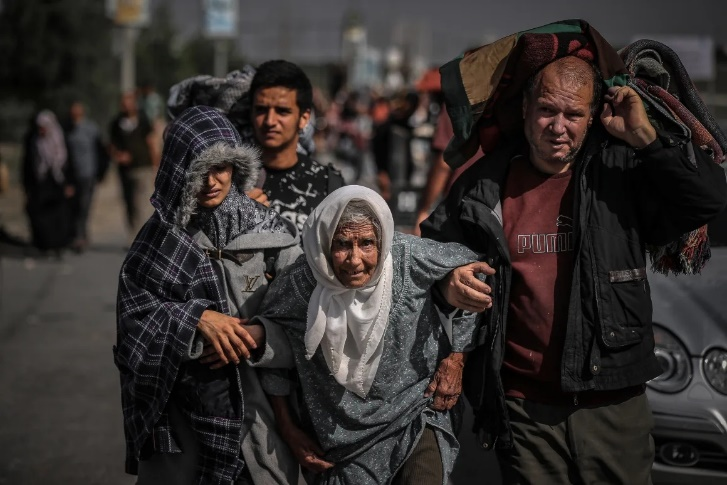
\includegraphics[width=3.30159in,height=2.2in]{media/media/image6.jpeg}
\end{minipage} & \begin{minipage}[b]{\linewidth}\centering
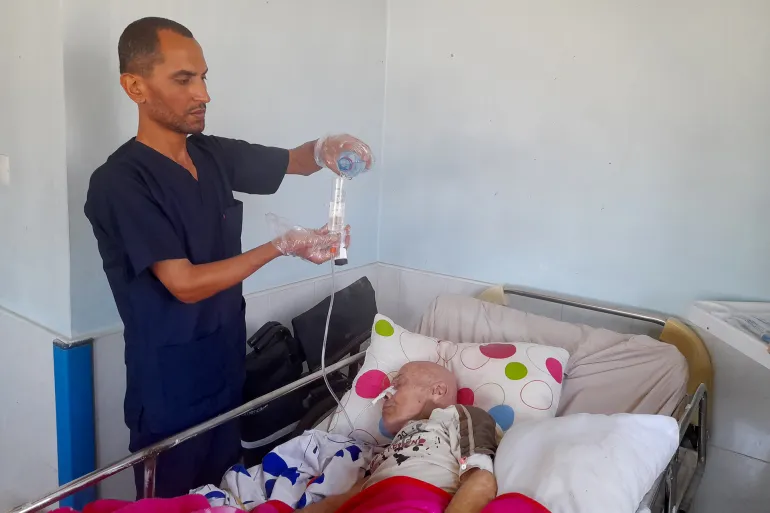
\includegraphics[width=3.23542in,height=2.59972in]{media/media/image7.png}
\end{minipage} \\
\midrule\noalign{}
\endhead
\bottomrule\noalign{}
\endlastfoot
\end{longtable}
}
\vspace{0.3em}
\noindent{\small\textbf{সূত্র:} Euro-Mediterranean Human Rights Monitor, \textit{Gaza's Elderly and Disabled Populations Face Disproportionate Death Toll Amid Ongoing Famine and Siege} (2024). \url{https://euromedmonitor.org/en/article/6452}}

একইসঙ্গে চলাচলে অক্ষমতা ও সহায়ক সরঞ্জামের অভাবে প্রতিবন্ধী ব্যক্তিরা বোমাবর্ষণ
বা জোরপূর্বক স্থানান্তরের সময় নিরাপদ স্থানে সরে যেতে পারছেন না, ফলে তারা
সহিংসতার সরাসরি শিকার হচ্ছেন। জাতিসংঘ মানবাধিকার দপ্তর (OHCHR) জানিয়েছে যে
অতিরিক্ত শক্তি প্রয়োগ, অবকাঠামো ধ্বংস এবং চিকিৎসা ও পুনর্বাসন সেবার অভাবে
গাজায় প্রতিবন্ধী মানুষের সংখ্যা উল্লেখযোগ্যভাবে বৃদ্ধি পেয়েছে, অথচ তাদের জন্য
প্রয়োজনীয় সহায়তা প্রায় অনুপস্থিত (\emph{OHCHR}, n.d.)। পারিবারিক ও
সম্প্রদায়ভিত্তিক সহায়তা কাঠামো ভেঙে পড়ায় এই জনগোষ্ঠী কার্যত একা ও অসহায় হয়ে
পড়েছে, যা অনাহার-কৌশলকে কেবল খাদ্যবঞ্চনা নয়, বরং সমাজের সবচেয়ে দুর্বল অংশের
জন্য নীরব ও কাঠামোগত মৃত্যুঝুঁকিতে পরিণত করেছে।

\subsection{\texorpdfstring{স্বাস্থ্য ব্যবস্থার পতন ও মহামারীর ঝুঁকি
}{৪.৪ স্বাস্থ্য ব্যবস্থার পতন ও মহামারীর ঝুঁকি }}\label{ux9b8ux9acux9b8ux9a5ux9af-ux9acux9afux9acux9b8ux9a5ux9b0-ux9aaux9a4ux9a8-ux993-ux9aeux9b9ux9aeux9b0ux9b0-ux99dux995}

\subsubsection{হাসপাতাল ও চিকিৎসা অবকাঠামোর
ধ্বংস}\label{ux9b9ux9b8ux9aaux9a4ux9b2-ux993-ux99aux995ux9ceux9b8-ux985ux9acux995ux9a0ux9aeux9b0-ux9a7ux9acux9b8}

{\def\LTcaptype{none} % do not increment counter
\begin{longtable}[]{@{}
  >{\raggedright\arraybackslash}p{(\linewidth - 2\tabcolsep) * \real{0.5000}}
  >{\raggedright\arraybackslash}p{(\linewidth - 2\tabcolsep) * \real{0.5000}}@{}}
\toprule\noalign{}
\begin{minipage}[b]{\linewidth}\raggedright
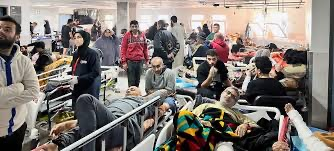
\includegraphics[width=3.47917in,height=2.1875in]{media/media/image8.jpg}
\end{minipage} & \begin{minipage}[b]{\linewidth}\raggedright
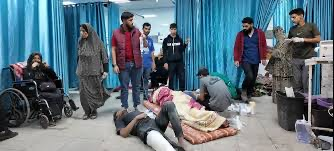
\includegraphics[width=3.47917in,height=2.17708in]{media/media/image9.jpg}
\end{minipage} \\
\midrule\noalign{}
\endhead
\bottomrule\noalign{}
\endlastfoot
\end{longtable}
}
\vspace{0.3em}
\noindent{\small\textbf{সূত্র:} World Health Organization (WHO), \textit{Health Cluster Bulletin: Gaza Strip} (May 2025). \url{https://www.emro.who.int/opt/information-resources/health-cluster-bulletins.html}}

গাজায় সংঘাতের ধারাবাহিকতা ও খাদ্য, জ্বালানি এবং চিকিৎসা সরবরাহে বাধার
কারণে স্বাস্থ্যব্যবস্থা প্রায় ভেঙে পড়েছে, এবং এর কেন্দ্রবিন্দুতে রয়েছে হাসপাতাল ও
চিকিৎসা অবকাঠামোর বিস্তৃত ধ্বংস ও অকার্যকারিতা। WHO-এর ২০২৫ সালের ২২ মে
প্রকাশিত বিবৃতিতে বলা হয়েছে যে গাজা স্ট্রিপের পূর্বে ৩৬টি হাসপাতালের মধ্যে মাত্র
১৯টি আংশিকভাবে কার্যকর আছে, যেখানে অধিকাংশই সরঞ্জাম, ওষুধ, জনশক্তি ও
নিরাপত্তা সংকটে ভুগছে এবং মাত্র কিছুই মৌলিক জরুরি সেবা দিতে সক্ষম হচ্ছে; প্রায়
৯৪\% হাসপাতাল ক্ষতিগ্রস্ত বা ধ্বংস হয়ে গেছে এবং বেশ কিছু হাসপাতাল, যেমন কামাল
আদওয়ান ও ইন্দোনেশিয়ান হাসপাতাল, সরাসরি সংঘাতে বন্ধ বা পরিষেবা স্থগিত করতে
হয়েছে তাদের আশেপাশে হিংসাত্মক অবস্থার কারণে। সেই সঙ্গে জ্বালানি, ওষুধ ও
গুরুত্বপূর্ণ চিকিৎসা যন্ত্রপাতির অভাব একটি সমগ্র স্বাস্থ্য ব্যবস্থার কার্যক্ষমতা সংকুচিত
করেছে---ভেন্টিলেটর, ডায়ালাইসিস মেশিন, অ্যানেস্থেশিয়া ওষুধ এবং অন্যান্য জরুরি
সরঞ্জামের ঘাটতি হাসপাতালে জীবন-রক্ষাকারী পরিষেবাকে প্রায় অচল করে দিয়েছে এবং
চিকিৎসক ও নার্সদের পেশাগত কাজকে অসম্ভাব্য পরিস্থিতিতে ঠেলে দিয়েছে। WHO
পর্যবেক্ষণ জানিয়েছে যে এই ধ্বংসের ধারাবাহিকতায় নাগরিকরা জটিল রোগের চিকিৎসা,
অস্ত্রোপচার ও মানসিক স্বাস্থ্য সেবা পাচ্ছে না, এবং স্বাস্থ্য কর্মীদের ওপর আক্রান্তি
ও নিরাপত্তার অভাব স্বাস্থ্যব্যবস্থাকে আরও দুর্বল করেছে, এমনকি হাসপাতালে কর্মরত
ব্যক্তিরাও হামলার শিকার হচ্ছেন। এই পরিস্থিতি শুধু পরিষেবা বন্ধই ঘটায়নি, বরং
গাজার বেশিরভাগ এলাকায় স্বাস্থ্য গ্রহণযোগ্যতা ও অ্যাক্সেসকে প্রায় অসম্ভাব্য করে
দিয়েছে, ফলে সাধারণ রোগ, দুর্ঘটনা এবং সংঘাত-সংক্রান্ত আহতদের সঠিক চিকিৎসা
পর্যন্ত পৌঁছানো বন্ধ হয়ে গেছে --- যা একটি স্বাস্থ্য ব্যবস্থার পুরোপুরি পতনের প্রমাণ
হিসেবে ধরা হচ্ছে এবং জাতিসংঘসহ আন্তর্জাতিক স্বাস্থ্য সংস্থাগুলোর কাছে তা
একাধিকবার ``ব্রেকিং পয়েন্ট'' বা ভাঙনবিন্দুতে পৌঁছে গেছে বলে ব্যাখ্যা করা হয়েছে
(\emph{Health System at Breaking Point as Hostilities Further Intensify
in Gaza, WHO Warns}, n.d.)

\subsubsection{রোগের
প্রাদুর্ভাব}\label{ux9b0ux997ux9b0-ux9aaux9b0ux9a6ux9b0ux9adux9ac}

গাজায় অবরুদ্ধ জীবনযাত্রা, পানি ও স্যানিটেশন ব্যবস্থার ধ্বংস এবং স্বাস্থ্যব্যবস্থার
পতনের প্রভাবে রোগের প্রাদুর্ভাব ব্যাপকভাবে বৃদ্ধি পেয়েছে এবং এটি একটি তীব্র
জনস্বাস্থ্য সংকটে পরিণত হচ্ছে; দূষিত পানি ও অপর্যাপ্ত স্যানিটেশন ব্যবস্থার কারণে
পানিবাহিত রোগ যেমন ডায়রিয়া ও সম্ভাব্য কলেরা মারাত্মকভাবে ছড়িয়ে পড়েছে---মধ্য
অক্টোবর ২০২৩ থেকে ৩৩,৫৫১টির বেশি ডায়রিয়া আক্রান্ত মামলার রিপোর্ট পাওয়া গেছে,
যেখানে অর্ধেকেরও বেশি ৫ বছরের কম বয়েসী শিশুদের মধ্যে হয়েছে, যা আগের গড়ের
তুলনায় বহুগুণ বেশি। অবরুদ্ধ পরিবেশে অতি-ঘন বসতি ও নিরাপদ পানি না থাকায়
ব্যাকটেরিয়াল সংক্রমণ সহজেই ছড়িয়ে যাচ্ছে, এবং বর্জ্য সংগ্রহ না হওয়ায় রোগজীবাণুর
পরিবেশ সৃষ্টি হচ্ছে যা ডায়রিয়া ছড়িয়ে দেয়। একই সঙ্গে ধুলো, দূষণ, ঠান্ডা আবহাওয়া
ও ভিড়ে বসবাসের কারণে শ্বাসতন্ত্রের সংক্রমণ---নিউমোনিয়া ও অন্যান্য শ্বাসকষ্টজনিত
রোগের হারের তীব্র বৃদ্ধি লক্ষ্য করা হচ্ছে। পাশাপাশি পানি, সাবান ও পরিষ্কার
থাকার সুযোগ কম থাকায় চর্মরোগ যেমন স্ক্যাবিস, ফাঙ্গাল ইনফেকশন ও অন্যান্য ত্বক
সংক্রমণ দ্রুত ছড়িয়ে পড়ে, বিশেষত শিশু ও অটল জনগোষ্ঠীর মধ্যে। স্বাস্থ্য ব্যবস্থা
ভাঙার কারণে নিয়মিত টিকাদান কর্মসূচি ও ইমিউনাইজেশনও ব্যাহত হয়েছে---ফসলানো
টিকা, পোলিও ও অন্যান্য প্রতিষেধক কার্যক্রম অসম, যার ফলে ডিপথের মতো
প্রতিষেধনযোগ্য রোগগুলি ফের ফিরে আসার ঝুঁকি তৈরি হয়েছে। এসব প্রাদুর্ভাবের পেছনে
শুধু চিকিৎসা পরিষেবার অভাব নয়, বরং নিরাপদ পানীয়, স্যানিটেশন, স্বাস্থ্য কেন্দ্র ও
টিকাদানের ব্যাহত কার্যক্রমের সমষ্টিগত ধ্বংসও দায়ী হিসেবে কাজ করছে, যা একটি
সহজেই প্রতিরোধযোগ্য জনস্বাস্থ্য বিপর্যয়কে একটি বিস্তৃত মহামারি-সদৃশ পরিস্থিতিতে
পরিণত করেছে (\emph{Life Course Immunization: Why Lifelong Vaccination Is
Essential for Public Health}, n.d.)।

\subsection{দীর্ঘমেয়াদী সামাজিক, অর্থনৈতিক ও মানসিক
প্রভাব}\label{ux9a6ux9b0ux998ux9aeux9dfux9a6-ux9b8ux9aeux99cux995-ux985ux9b0ux9a5ux9a8ux9a4ux995-ux993-ux9aeux9a8ux9b8ux995-ux9aaux9b0ux9adux9ac}

\subsubsection{সামাজিক কাঠামো
ধ্বংস}\label{ux9b8ux9aeux99cux995-ux995ux9a0ux9ae-ux9a7ux9acux9b8}

গাজার বিস্তৃত বনধ্বংস, ভগ্ন-পূনর্বাসন ও দীর্ঘমেয়াদি সংঘাত অনাহারসহ সামগ্রিক
মানবিক সংকট সমাজের সামাজিক কাঠামোকে মূলভিত্তিতে নিক্ষেপ করেছে; হাজার হাজার
পরিবার সদস্যদের বিচ্ছিন্ন হতে বাধ্য হয়েছে এবং বহু শিশু পিতামাতা বা অভিভাবক
হারিয়েছে, ফলে পরিবার নামক মৌলিক সামাজিক ইউনিটের ঐক্য ও নিরাপত্তা ভঙ্গ
হয়েছে, যা প্রজন্মগত মানসিক ও সামাজিক ক্ষতির সূচনা করেছে। পাশাপাশি এই দীর্ঘ
সংকটের ফলে সমাজের ঐক্য ও পারস্পরিক সহযোগিতার যোগসাজশও ক্ষতিগ্রস্ত হয়েছে; এক
সময়ে ঘনিষ্ঠ ও পরস্পর নির্ভরশীল গাজা সমাজ এখন বারবার স্থানান্তর, নিরাপত্তাহীনতা
ও জীবিকার জন্য প্রতিযোগিতার কারণে ভাঙাচোরা হয়ে পড়ছে, এবং ঘর-বাড়ি, বাজার ও
সামাজিক স্থানগুলোর ধ্বংস সামাজিক বন্ধনকে দুর্বল করে তুলেছে। গাজার অবকাঠামোর
ব্যাপক ধ্বংসে প্রায় ছয় থেকে আট শতাংশের বেশি ভবন ক্ষতিগ্রস্ত বা ধ্বংস হয়েছে, যার
মধ্যে বহু পরিবারকে তাদের ঐতিহ্য, ভূমি ও সামাজিক নেটওয়ার্ক থেকে বিচ্ছিন্ন হতে
বাধ্য করেছে; এটি শুধু যুদ্ধের ক্ষতি হিসেবেই নয়, বরং সম্প্রদায়ের ভিত্তিক ঐক্য ও
সংহতি ভাঙার একটি অদৃশ্য সামাজিক বিপর্যয় হিসেবে বিবেচিত হচ্ছে। শিক্ষা ব্যবস্থাও
প্রাণবন্ত থাকতে পারেনি; ৯৭ শতাংশ স্কুল ও শিক্ষা প্রতিষ্ঠান ক্ষতিগ্রস্ত বা ধ্বংস
হওয়ার কারণে শিশু ও যুবসমাজের শিক্ষাগত প্রগতি অবরুদ্ধ হয়েছে, এবং অনলাইন শিক্ষা
বা বিকল্প ব্যবস্থা চালু করার জন্য প্রয়োজনীয় বিদ্যুৎ ও ইন্টারনেটের প্রতিও প্রবেশ
সীমিত থাকায় শিশু ও কিশোরদের শিক্ষা থেকে দীর্ঘমেয়াদী বঞ্চনার ঝুঁকি তৈরি হয়েছে,
যা সমাজের সামগ্রিক পুনর্গঠনের সম্ভাবনাকেও হ্রাস করছে। এই বিশৃঙ্খল পরিবেশে
পরিবার, সম্প্রদায় ও শিক্ষা---সমাজের তিনটি মূল স্তম্ভ---একসাথে পদ্ধতিগতভাবে ধ্বংস
ও বিচ্ছিন্ন হয়ে যাচ্ছে, যার প্রভাব কেবল সমকালীন মানবিক বিপর্যয়ে সীমাবদ্ধ থাকবে
না, বরং প্রজন্ম ধরে সমাজের মৌলিক গঠন ও মানবিক সম্পর্কগুলোকে দুর্বল করবে
(\emph{UN News}, n.d.)

\subsubsection{\texorpdfstring{৪.৫.২ অর্থনৈতিক ধ্বংস
}{৪.৫.২ অর্থনৈতিক ধ্বংস }}\label{ux985ux9b0ux9a5ux9a8ux9a4ux995-ux9a7ux9acux9b8}

গাজায় অনাহার-কৌশল, অবরোধ ও ব্যাপক ধ্বংসযজ্ঞের প্রত্যক্ষ ফল হিসেবে সম্পূর্ণ
অর্থনৈতিক ব্যবস্থা কার্যত ভেঙে পড়েছে\textbf{,} যেখানে উৎপাদন, কর্মসংস্থান ও
বাজার---এই তিনটি স্তম্ভই একযোগে ধ্বংসপ্রাপ্ত হয়েছে। কৃষি ও উৎপাদন খাতে ভয়াবহ
ক্ষতি সাধিত হয়েছে; কৃষিজমি, গ্রীনহাউস, সেচব্যবস্থা, মৎস্য খামার এবং ক্ষুদ্র
শিল্পগুলো লক্ষ্যবস্তু হওয়ায় গাজার ৫০ শতাংশের বেশি কৃষি অবকাঠামো ক্ষতিগ্রস্ত বা
ধ্বংস হয়েছে, যার ফলে স্থানীয় খাদ্য উৎপাদন প্রায় বন্ধ হয়ে গেছে এবং জনগণ
সম্পূর্ণভাবে আমদানিনির্ভর ও ত্রাণনির্ভর হয়ে পড়েছে (FAO)। একই সঙ্গে শিল্প, বাণিজ্য
ও সেবা খাত অচল হয়ে পড়ায় কর্মসংস্থানের সুযোগ কার্যত বিলুপ্ত হয়েছে; আন্তর্জাতিক
শ্রম সংস্থা (ILO) অনুযায়ী গাজায় বেকারত্বের হার ৯০ শতাংশেরও বেশি, যা আধুনিক
ইতিহাসে বিরল এবং একটি সম্পূর্ণ জনগোষ্ঠীকে আয়ের কোনো উৎস ছাড়াই বেঁচে থাকতে
বাধ্য করছে। এই বাস্তবতায় গাজার অর্থনীতি কেবল সংকুচিত নয়, বরং সম্পূর্ণ স্থবির ও
পতিত অবস্থায় পৌঁছেছে; জাতিসংঘের বাণিজ্য ও উন্নয়ন সংস্থা (UNCTAD) জানিয়েছে যে
২০২৪ সালে গাজার অর্থনীতি ৮৩ শতাংশ সংকুচিত হয়েছে, যার ফলে প্রায় ২৩ লাখ মানুষ
দারিদ্র্যসীমার নিচে নেমে গেছে এবং মাথাপিছু আয় নেমে এসেছে বছরে প্রায় ১৬১
মার্কিন ডলারে---বিশ্বের সর্বনিম্ন পর্যায়ের মধ্যে একটি (\emph{UN Trade and
Development (UNCTAD)}, 2024)। অবরোধের কারণে পুনর্গঠনের জন্য প্রয়োজনীয়
নির্মাণসামগ্রী, যন্ত্রপাতি ও কাঁচামাল আমদানিও সম্ভব হচ্ছে না, ফলে অর্থনৈতিক
পুনরুদ্ধারের ন্যূনতম শর্তগুলো পর্যন্ত অনুপস্থিত; এর ফলে গাজার জনগোষ্ঠী একটি স্থায়ী
দারিদ্র্য, ত্রাণনির্ভরতা ও অর্থনৈতিক অবরুদ্ধতার চক্রে আটকে পড়েছে, যা
অনাহার-কৌশলের দীর্ঘমেয়াদি ও কাঠামোগত প্রভাবকে আরও গভীরভাবে প্রমাণ করে।

\subsubsection{৪.৫.৩ মানসিক স্বাস্থ্যের উপর
প্রভাব}\label{ux9aeux9a8ux9b8ux995-ux9b8ux9acux9b8ux9a5ux9afux9b0-ux989ux9aaux9b0-ux9aaux9b0ux9adux9ac}

গাজা যুদ্ধের দীর্ঘস্থায়ী ও তীব্র সহিংসতা, ব্যাপক ধ্বংসযজ্ঞ, বাস্তুচ্যুতি এবং
পরিবার-প্রিয়জন হারানোর ফলে সমগ্র জনগোষ্ঠী এক গভীর সমষ্টিগত ট্রমা (collective
trauma) এর মধ্যে নিমজ্জিত হয়েছে। এই ট্রমা শুধু ব্যক্তিগত নয়, বরং পুরো সমাজ ও
সম্প্রদায়ের মানসিক কাঠামোকে ছিন্নভিন্ন করে দিয়েছে। নিরাপত্তাহীনতা, অবিরাম ভয়,
শোক এবং অনিশ্চয়তা এখন দৈনন্দিন জীবনের অবিচ্ছেদ্য অংশ হয়ে দাঁড়িয়েছে, যা মানুষের
মধ্যে চরম অসহায়ত্ব, হতাশা এবং অস্তিত্বের সংকট সৃষ্টি করেছে। WHO-এর একটি
ন্যারেটিভ রিভিউ (২০২৫) অনুসারে, গাজার চলমান সংঘাত (২০২৩ অক্টোবর থেকে)
জনগণের মানসিক স্বাস্থ্য ও সাইকোসোশ্যাল সুস্থতার উপর গভীর নেতিবাচক প্রভাব
ফেলেছে, যেখানে PTSD, ডিপ্রেশন এবং অ্যাঙ্গজাইটির হার অত্যন্ত উচ্চ---শিশুদের মধ্যে
PTSD ৫৪\%, ডিপ্রেশন ৪১\% এবং অ্যাঙ্গজাইটি ৩৪\% পর্যন্ত দেখা গেছে (পূর্ববর্তী
গবেষণা থেকে উদ্ধৃত), এবং প্রাপ্তবয়স্কদের মধ্যে এই হার যথাক্রমে ৪০\%, ৪৫\% এবং
৩৭\%। (\emph{World Health Organization}, 2025)
 এই সমষ্টিগত ট্রমা পরিবারের সংহতি ভেঙে দিয়েছে, সামাজিক নেটওয়ার্ক ধ্বংস
করেছে এবং সম্প্রদায়ের মধ্যে অবিশ্বাস ও পরিচয়ের সংকট তৈরি করেছে। আশাহীনতা,
ক্রমাগত দুর্ভোগ এবং ভবিষ্যতের প্রতি কোনো আলো না দেখার কারণে আত্মহত্যার প্রবণতা ও
চেষ্টা উল্লেখযোগ্যভাবে বৃদ্ধি পেয়েছে। UNICEF এবং Save the Children-এর পূর্ববর্তী
জরিপে (২০২২) দেখা গেছে যে গাজার শিশুদের মধ্যে প্রায় অর্ধেক আত্মহত্যার চিন্তা
করেছে এবং তিন-পঞ্চমাংশ সেল্ফ-হার্ম করেছে; বর্তমান যুদ্ধ এই প্রবণতাকে আরও তীব্র
করেছে। বিভিন্ন গবেষণায় (২০২৪-২০২৫) উল্লেখ করা হয়েছে যে যুদ্ধ-সংক্রান্ত ট্রমা,
বাস্তুচ্যুতি এবং ক্ষুধা-অপুষ্টির সমন্বয় মানসিক সংকটকে চরমে নিয়ে গেছে, যার ফলে
ডিপ্রেশনের হার কিছু স্টাডিতে ৯৯.৫\% পর্যন্ত রিপোর্ট করা হয়েছে।

সবচেয়ে ভয়াবহ দিক হলো প্রজন্মগত ট্রমা (intergenerational trauma)। শিশু ও তরুণ
প্রজন্মের উপর এই ট্রমার প্রভাব দীর্ঘমেয়াদী এবং বহুমুখী---তাদের মধ্যে আবেগ
নিয়ন্ত্রণের অক্ষমতা, মালঅ্যাডাপটিভ কোপিং মেকানিজম এবং বিকাশগত ব্যাঘাত দেখা
যাচ্ছে। WHO রিভিউতে উল্লেখ করা হয়েছে যে বারবার ট্রমা এক্সপোজারের ফলে জৈবিক
স্ট্রেস রেসপন্স পরিবর্তিত হয়ে ভবিষ্যৎ প্রজন্মের মনস্তাত্ত্বিক স্থিতিশীলতাকে প্রভাবিত
করে, যা প্যারেন্টিং প্যাটার্ন এবং পরিবারের মাধ্যমে ট্রান্সমিট হয়। UNICEF-এর
রিপোর্ট অনুসারে, গাজার প্রায় ১.২ মিলিয়ন শিশু এখন জরুরি মানসিক সহায়তার প্রয়োজন,
কিন্তু মানসিক স্বাস্থ্য সেবা প্রায় অস্তিত্বহীন---হাসপাতালের অভাব, বিশেষজ্ঞের
ঘাটতি এবং স্টিগমা এই সংকটকে আরও গভীর করেছে। ফলে, এই প্রজন্ম একটি "হারানো
প্রজন্ম"-এ পরিণত হওয়ার ঝুঁকিতে রয়েছে, যার দীর্ঘমেয়াদী প্রভাব গাজার সামাজিক,
অর্থনৈতিক ও মানসিক পুনর্গঠনের পথে বড় বাধা হয়ে দাঁড়াবে (Aqtam, 2025) (Taha et
al., 2024)।

\subsection{ভবিষ্যৎ প্রজন্মের উপর দীর্ঘমেয়াদী
প্রভাব}\label{ux9adux9acux9b7ux9afux9ce-ux9aaux9b0ux99cux9a8ux9aeux9b0-ux989ux9aaux9b0-ux9a6ux9b0ux998ux9aeux9dfux9a6-ux9aaux9b0ux9adux9ac}

\subsubsection{\texorpdfstring{৪.৬.১ হারানো প্রজন্ম
}{৪.৬.১ হারানো প্রজন্ম }}\label{ux9b9ux9b0ux9a8-ux9aaux9b0ux99cux9a8ux9ae}

গাজার বর্তমান শিশু ও কিশোররা এক ভয়াবহ মানবিক সংকটের মধ্য দিয়ে যাচ্ছে, যা
তাদের একটি ``হারানো প্রজন্মে'' পরিণত করার ঝুঁকি তৈরি করেছে। ক্যেমব্রিজ
বিশ্ববিদ্যালয়ের একটি প্রতিবেদন অনুযায়ী, গাজার শিশুরা ইতিমধ্যে প্রায় পাঁচ বছরের
সমপরিমাণ শিক্ষা জীবন হারিয়েছে---যার শুরু হয়েছিল কোভিড-১৯ মহামারি থেকে এবং
বর্তমান যুদ্ধের ধ্বংসলীলায় যা চূড়ান্ত পর্যায়ে পৌঁছেছে। অক্টোবর ২০২৫ পর্যন্ত পাওয়া
তথ্যমতে, ১৮,০০০-এর বেশি শিক্ষার্থী এবং প্রায় ৮০০ জন শিক্ষক প্রাণ হারিয়েছেন এবং
প্রায় ৯০\% স্কুল ভবন ক্ষতিগ্রস্ত বা ধ্বংস হয়েছে (\emph{Education in Gaza: A
``Lost'' Generation}, n.d.)। শিক্ষার এই অভাব কেবল অক্ষরজ্ঞানের ক্ষতি নয়, বরং
এটি শিশুদের পুষ্টি এবং মানসিক স্বাস্থ্যের ওপরও সরাসরি প্রভাব ফেলছে। কারণ,
স্কুলগুলো অনেক ক্ষেত্রে তাদের জন্য নিরাপদ আশ্রয় ও খাদ্য সরবরাহের কেন্দ্র ছিল।
দীর্ঘস্থায়ী অনাহার ও অপুষ্টির ফলে শিশুদের শারীরিক ও জ্ঞানীয় বিকাশ (cognitive
development) মারাত্মকভাবে বাধাগ্রস্ত হচ্ছে, যা ভবিষ্যতে তাদের কর্মদক্ষতা ও
সৃজনশীলতাকে পঙ্গু করে দেবে। এই বিশাল শূন্যতা পূরণ করা না গেলে, ভবিষ্যৎ গাজাকে
নেতৃত্ব দেওয়ার মতো দক্ষ জনশক্তির চরম অভাব দেখা দেবে।

\subsubsection{\texorpdfstring{৪.৬.২ পুনর্গঠনের চ্যালেঞ্জ
}{৪.৬.২ পুনর্গঠনের চ্যালেঞ্জ }}\label{ux9aaux9a8ux9b0ux997ux9a0ux9a8ux9b0-ux99aux9afux9b2ux99eux99c}

গাজার পুনর্গঠন প্রক্রিয়া কেবল দালানকোঠা নির্মাণের বিষয় নয়, এটি একটি
দীর্ঘমেয়াদী ও জটিল আর্থ-সামাজিক চ্যালেঞ্জ। ব্রুকিংস ইনস্টিটিউশনের বিশ্লেষণ
অনুযায়ী, যুদ্ধের ফলে গাজায় প্রায় ৫০ মিলিয়ন টনেরও বেশি ধ্বংসস্তূপ (debris) তৈরি
হয়েছে, যা পরিষ্কার করতেই প্রায় ২০ বছর সময় লেগে যেতে পারে। আবাসন, অবকাঠামো
ও অর্থনীতিকে যুদ্ধের আগের অবস্থায় ফিরিয়ে নিতে কমপক্ষে ৪০ থেকে ৫০ বিলিয়ন ডলার
প্রয়োজন এবং এই প্রক্রিয়া কয়েক দশক ধরে চলতে পারে (\emph{Gaza's Day after:
Reconstruction and Governance Challenges \textbar{} Brookings}, n.d.)।
পুনর্গঠনের প্রধান বাধাগুলোর মধ্যে রয়েছে গাজার মেধাবী ও দক্ষ পেশাজীবীদের
(শিক্ষক, ডাক্তার, প্রকৌশলী) দেশত্যাগ বা ``ব্রেইন ড্রেইন'', যা পুনর্গঠন কাজের
গতিকে মন্থর করে দেবে। এছাড়া, আন্তর্জাতিক সাহায্য সংস্থাগুলোর জন্য বড় চ্যালেঞ্জ
হলো গাজার প্রশাসনিক ও রাজনৈতিক অস্থিতিশীলতা। দাতা দেশগুলো দীর্ঘমেয়াদী
বিনিয়োগের ক্ষেত্রে নিরাপত্তা ও নিশ্চয়তা চায়, যাতে পুনরায় ধ্বংসের চক্রে পড়তে না
হয়। শিক্ষা, স্বাস্থ্য ও কর্মসংস্থান পুনরুদ্ধারে আন্তর্জাতিক সম্প্রদায়ের কেবল আর্থিক
সহায়তাই নয়, বরং রাজনৈতিক সমাধান ও প্রশাসনিক কাঠামোর দীর্ঘমেয়াদী সংস্কার
প্রয়োজন।

\subsection{উপসংহার}\label{ux989ux9aaux9b8ux9b9ux9b0-ux98fux995ux99f-ux997ux9a3-ux9aeux9a8ux9acux995-ux9acux9aaux9b0ux9afux9dfux9b0-ux9a6ux9b2ux9b2}

উপরে আলোচিত বিশ্লেষণ থেকে এটি স্পষ্ট যে, ২০২৩-২০২৫ সালের গাজা যুদ্ধে ইসরাইলের
গৃহীত `অনাহার-কৌশল' কেবল একটি সামরিক কৌশল নয়, বরং এটি একটি সুপরিকল্পিত
গণ-মানবিক বিপর্যয়ের ব্লুপ্রিন্ট। এই অধ্যায়ে আমরা দেখেছি কীভাবে খাদ্য, পানি এবং
চিকিৎসাকে অস্ত্র হিসেবে ব্যবহার করে একটি সমগ্র জনপদকে ধ্বংসের মুখে ঠেলে দেওয়া
হয়েছে।

এই বিপর্যয়ের দলিল হিসেবে কয়েকটি মূল বিষয়কে উপসংহারে গুরুত্ব দেওয়া প্রয়োজন:

\begin{itemize}
\item
  \textbf{পরিকল্পিত ধ্বংসযজ্ঞ:} গাজার কৃষি জমি, মৎস্য শিল্প এবং খাদ্য উৎপাদন
  অবকাঠামোর পদ্ধতিগত ধ্বংস প্রমাণ করে যে, এটি কেবল হামাসকে লক্ষ্য করে
  পরিচালিত কোনো অভিযান ছিল না। বরং এর উদ্দেশ্য ছিল গাজার জনগণের টিকে থাকার
  নূন্যতম সক্ষমতাটুকু কেড়ে নেওয়া।
\item
  \textbf{মানবাধিকারের চরম লঙ্ঘন:} আন্তর্জাতিক সম্প্রদায় ও বিভিন্ন মানবাধিকার
  সংস্থার বারবার সতর্কবাণী সত্ত্বেও জীবনরক্ষাকারী ত্রাণের প্রবেশে বাধা দেওয়া
  হয়েছে। এর ফলে সৃষ্ট তীব্র অপুষ্টি ও দুর্ভিক্ষ-সদৃশ পরিস্থিতি প্রমাণ করে যে, এখানে
  আন্তর্জাতিক মানবিক আইন ) এবং জেনেভা কনভেনশনকে বৃদ্ধাঙ্গুলি দেখানো হয়েছে।
\item
  \textbf{ভবিষ্যৎ প্রজন্মের অপূরণীয় ক্ষতি:} ``হারানো প্রজন্ম'' তৈরির যে ঝুঁকি
  আমরা আলোচনা করেছি, তা এই সংকটের সবচেয়ে দীর্ঘস্থায়ী ও বেদনাদায়ক ফলাফল।
  শিক্ষা থেকে বিচ্যুতি, শারীরিক পঙ্গুত্ব এবং মানসিক ট্রমা গাজার শিশুদের এমন এক
  অন্ধকারে ঠেলে দিয়েছে, যা থেকে উত্তরণে কয়েক দশক লেগে যেতে পারে।
\item
  \textbf{বিশ্ব বিবেকের দায়বদ্ধতা:} গাজার এই মানবিক বিপর্যয় বিশ্ব ইতিহাসের
  পাতায় একটি কালো অধ্যায় হিসেবে চিহ্নিত হয়ে থাকবে। পুনর্গঠনের বিশাল চ্যালেঞ্জ
  এবং সামাজিক কাঠামো পুনরুদ্ধারে আন্তর্জাতিক সম্প্রদায়ের কেবল মৌখিক সহানুভূতি নয়,
  বরং দীর্ঘমেয়াদী এবং কার্যকরী প্রতিশ্রুতি এখন সময়ের দাবি।
\end{itemize}

পরিশেষে বলা যায়, এই অধ্যায়ে বর্ণিত প্রভাব ও ফলাফলগুলো কেবল পরিসংখ্যান নয়;
এগুলো একটি জীবন্ত জাতির অস্তিত্ব রক্ষার লড়াই এবং সমকালীন বিশ্বের সবচেয়ে বড়
মানবিক ব্যর্থতার দলিল।

\section{পঞ্চম অধ্যায়: আন্তর্জাতিক
প্রতিক্রিয়া}\label{ux9aaux99eux99aux9ae-ux985ux9a7ux9afux9df-ux986ux9a8ux9a4ux9b0ux99cux9a4ux995-ux9aaux9b0ux9a4ux995ux9b0ux9df}

\subsection{জাতিসংঘের
ভূমিকা}\label{ux99cux9a4ux9b8ux998ux9b0-ux9adux9aeux995}

\subsubsection{সতর্কীকরণ: মানবিক বিপর্যয়ের আগাম
সংকেত}\label{ux9b8ux9a4ux9b0ux995ux995ux9b0ux9a3-ux9aeux9a8ux9acux995-ux9acux9aaux9b0ux9afux9dfux9b0-ux986ux997ux9ae-ux9b8ux995ux9a4}

গাজার সংকটের ভয়াবহতা সম্পর্কে আন্তর্জাতিক সম্প্রদায়কে সতর্ক করার ক্ষেত্রে
জাতিসংঘের মানবিক ও বিশেষায়িত সংস্থাসমূহ একটি গুরুত্বপূর্ণ নৈতিক ও তথ্যগত ভূমিকা
পালন করেছে। United Nations Office for the Coordination of Humanitarian
Affairs, World Food Programme, UNICEF এবং World Health Organization
ধারাবাহিকভাবে গাজার খাদ্য নিরাপত্তাহীনতা, শিশু অপুষ্টি, পানিবাহিত রোগ,
স্বাস্থ্যব্যবস্থার পতন এবং মৃত্যুহারের উপর নির্ভরযোগ্য ও বিশ্লেষণভিত্তিক তথ্য প্রকাশ
করেছে। এই সংস্থাগুলোর প্রতিবেদন গাজায় অনাহারের ধীরে ধীরে ``মানবসৃষ্ট
দুর্ভিক্ষে'' রূপ নেওয়ার প্রক্রিয়াকে বিশ্ববাসীর সামনে স্পষ্টভাবে তুলে ধরে। বিশেষ
করে শিশুদের মধ্যে তীব্র অপুষ্টির হার বৃদ্ধি, হাসপাতালগুলোর কার্যত অচল হয়ে পড়া এবং
নিরাপদ পানির তীব্র সংকট---এই সবকিছুই তাদের সতর্কবার্তায় ধারাবাহিকভাবে
প্রতিফলিত হয়েছে।

জাতিসংঘের সর্বোচ্চ পর্যায় থেকেও এই সংকট সম্পর্কে কঠোর ও স্পষ্ট সতর্কবার্তা প্রদান
করা হয়েছে। অহঃষ্টহরড় এবং উল্লেখ করেছেন যে গাজার পরিস্থিতি দদধ
humanitarian catastrophe'' এবং ``a crisis of humanity'' হিসেবে বিবেচিত
হওয়া উচিত। তিনি আরও সতর্ক করে বলেন যে, বেসামরিক জনগণের জন্য নিরাপদ পানি,
খাদ্য ও জ্বালানির অভাব একটি ``collective punishment''-এর শামিল হতে পারে,
যা আন্তর্জাতিক মানবিক আইনের মৌলিক নীতির সঙ্গে অসামঞ্জস্যপূর্ণ \emph{(UN Press
Briefings and Statements on Gaza Crisis (2023--2024))}।

একইভাবে, জাতিসংঘের মানবাধিকার বিষয়ক হাইকমিশনার ঠড়ষশবৎ ঞহৃৎশ গাজায় চলমান
পরিস্থিতিকে আন্তর্জাতিক আইনের সম্ভাব্য গুরুতর লঙ্ঘন হিসেবে আখ্যায়িত করে বলেন যে,
মানবিক সহায়তা বাধাগ্রস্ত করা এবং বেসামরিক অবকাঠামো ধ্বংস করা ``may amount
to war crimes''। তিনি বিশেষভাবে খাদ্য ও পানির প্রবেশাধিকার সীমিত করার ফলে
সৃষ্ট পরিস্থিতিকে গভীর উদ্বেগের কারণ হিসেবে তুলে ধরেন (\emph{ঠড়ষশবৎ ঞহৃৎশ,
OHCHR Statements on Gaza (2023--2024}))।

এছাড়া, Martin Griffiths (OCHA প্রধান) গাজার পরিস্থিতিকে ``beyond
catastrophic'' হিসেবে বর্ণনা করে সতর্ক করেছেন যে, যদি মানবিক সহায়তার অবাধ
প্রবেশ নিশ্চিত না করা হয়, তবে এটি দ্রুত একটি পূর্ণাঙ্গ দুর্ভিক্ষে পরিণত হতে পারে।
একই ধরনের উদ্বেগ Catherine Russell ব্যক্ত করেন, যিনি শিশুদের মধ্যে অপুষ্টি ও
মৃত্যুঝুঁকি নিয়ে গভীর উদ্বেগ প্রকাশ করে বলেন যে, গাজায় ``children are paying
the highest price''।

তবে এই উচ্চপর্যায়ের সতর্কীকরণ ও ধারাবাহিক প্রতিবেদন সত্ত্বেও জাতিসংঘ সংস্থাগুলোর
কার্যক্রম মূলত তথ্য সংগ্রহ, পরিস্থিতি নথিভুক্তকরণ এবং সীমিত মানবিক সহায়তা
প্রদানের মধ্যেই সীমাবদ্ধ থেকেছে। তারা সরাসরি রাজনৈতিক সিদ্ধান্ত গ্রহণ, অবরোধ
প্রত্যাহার বা সামরিক কার্যক্রম বন্ধ করার ক্ষমতা রাখে না। ফলে একদিকে তারা
সংকটের গভীরতা অত্যন্ত নিখুঁতভাবে তুলে ধরতে সক্ষম হলেও, অন্যদিকে সেই তথ্য কার্যকর
রাজনৈতিক পদক্ষেপে রূপান্তরিত করতে ব্যর্থ হয়েছে।

এই বাস্তবতা আন্তর্জাতিক ব্যবস্থার একটি কাঠামোগত সীমাবদ্ধতাকে স্পষ্ট করে---যেখানে
মানবিক সত্য ও সতর্কবার্তা জোরালোভাবে উচ্চারিত হলেও, তা প্রায়শই রাজনৈতিক
স্বার্থ, ভেটো ক্ষমতা এবং ভূ-রাজনৈতিক বিভাজনের কারণে কার্যকর প্রতিরোধমূলক
পদক্ষেপে পরিণত হয় না। গাজার প্রেক্ষাপটে এই বিচ্ছিন্নতা বিশেষভাবে স্পষ্ট, যেখানে
``early warning'' থাকা সত্ত্বেও ``early action'' অনুপস্থিত ছিল।

\subsubsection{নিরাপত্তা পরিষদের
অচলাবস্থা}\label{ux9a8ux9b0ux9aaux9a4ux9a4-ux9aaux9b0ux9b7ux9a6ux9b0-ux985ux99aux9b2ux9acux9b8ux9a5}

জাতিসংঘ নিরাপত্তা পরিষদ (UNSC) আন্তর্জাতিক শান্তি ও নিরাপত্তা রক্ষার সর্বোচ্চ
কর্তৃত্বশীল সংস্থা হওয়া সত্ত্বেও গাজা সংকটে এটি কার্যত অচল ও নিষ্ক্রিয় প্রমাণিত
হয়েছে। গাজায় তাৎক্ষণিক ও স্থায়ী যুদ্ধবিরতি, অবরোধ শিথিলকরণ কিংবা মানবিক
করিডোর নিশ্চিত করার মতো প্রস্তাবগুলো বারবার উত্থাপিত হলেও, যুক্তরাষ্ট্রসহ কিছু
স্থায়ী সদস্য রাষ্ট্রের ভেটো ক্ষমতা প্রয়োগের কারণে সেগুলো বাধ্যতামূলক সিদ্ধান্তে রূপ
নিতে পারেনি। এর ফলে নিরাপত্তা পরিষদ কেবল কিছু অ-বাধ্যতামূলক (non-binding)
বিবৃতি ও প্রস্তাব গ্রহণে সীমাবদ্ধ থেকেছে, যা মাঠপর্যায়ে কোনো বাস্তব পরিবর্তন
আনতে ব্যর্থ হয়েছে।

এই অচলাবস্থা কেবল একটি প্রাতিষ্ঠানিক ব্যর্থতা নয়; বরং এটি আন্তর্জাতিক ব্যবস্থার
গভীর রাজনৈতিক সংকটের প্রতিফলন। যেখানে একটি জনগোষ্ঠী অনাহার, রোগ ও ধ্বংসের
মুখোমুখি, সেখানে নিরাপত্তা পরিষদের নীরবতা বা অকার্যকারিতা মানবিক আইন ও নৈতিক
দায়িত্বের প্রতি আন্তর্জাতিক সম্প্রদায়ের অবহেলারই প্রমাণ দেয়। এর ফলে জাতিসংঘের
বিশ্বাসযোগ্যতা প্রশ্নের মুখে পড়েছে এবং এটি স্পষ্ট হয়েছে যে শক্তিধর রাষ্ট্রগুলোর
ভূ-রাজনৈতিক স্বার্থ মানবিক ন্যায়বিচারের চেয়ে প্রাধান্য পাচ্ছে। গাজা সংকটে
নিরাপত্তা পরিষদের এই ব্যর্থতা ভবিষ্যতের আন্তর্জাতিক জবাবদিহিতার কাঠামো নিয়েও
গুরুতর প্রশ্ন উত্থাপন করে।

\subsection{আন্তর্জাতিক আদালত ও বিচারিক
প্রক্রিয়া}\label{ux986ux9a8ux9a4ux9b0ux99cux9a4ux995-ux986ux9a6ux9b2ux9a4-ux993-ux9acux99aux9b0ux995-ux9aaux9b0ux995ux9b0ux9df}

গাজা সংকটে আইনি জবাবদিহিতার প্রধান ক্ষেত্র হিসেবে আন্তর্জাতিক আদালতগুলো ক্রমশ
গুরুত্বপূর্ণ হয়ে উঠেছে। আন্তর্জাতিক ন্যায়বিচার আদালত (ICJ), আন্তর্জাতিক ফৌজদারি
আদালত (ICC) এবং কিছু রাষ্ট্রের জাতীয় আদালতে সর্বজনীন এখতিয়ার প্রয়োগ---এই
তিনটি স্তরেই আইনি উদ্যোগ দেখা গেছে। তবে এসব বিচারিক প্রক্রিয়ার গতি অত্যন্ত
ধীর, বাস্তবায়ন ক্ষমতা সীমিত এবং রাজনৈতিক প্রতিবন্ধকতা প্রবল, যার ফলে
ন্যায়বিচারের ফলাফল এখনও অনিশ্চিত রয়ে গেছে।

\subsubsection{আন্তর্জাতিক ন্যায়বিচার আদালত (ICJ): দক্ষিণ আফ্রিকার
মামলা ও এর
তাৎপর্য}\label{ux986ux9a8ux9a4ux9b0ux99cux9a4ux995-ux9a8ux9afux9dfux9acux99aux9b0-ux986ux9a6ux9b2ux9a4-icj-ux9a6ux995ux9b7ux9a3-ux986ux9abux9b0ux995ux9b0-ux9aeux9aeux9b2-ux993-ux98fux9b0-ux9a4ux9ceux9aaux9b0ux9af}

আন্তর্জাতিক ন্যায়বিচার আদালতে (ICJ) দক্ষিণ আফ্রিকার দায়ের করা মামলা গাজা
সংকটের আইনি ইতিহাসে একটি যুগান্তকারী পদক্ষেপ হিসেবে বিবেচিত হয়। আদালত তার
প্রাথমিক আদেশে ইসরাইলের বিরুদ্ধে উত্থাপিত গণহত্যার অভিযোগকে ``সম্ভাব্য''
(plausible) বলে মন্তব্য করে এবং এই ভিত্তিতে ছয়টি অস্থায়ী ব্যবস্থা (Provisional
Measures) গ্রহণের নির্দেশ দেয়। এসব ব্যবস্থার মধ্যে ছিল---গণহত্যামূলক কর্মকাণ্ড ও
উসকানি বন্ধ করা, গাজায় বেসামরিক জনগণের জন্য মানবিক সহায়তা ও মৌলিক সেবার
প্রবেশ নিশ্চিত করা, এবং সম্ভাব্য যুদ্ধাপরাধ ও গণহত্যার প্রমাণ সংরক্ষণ করা।

এই আদেশের গুরুত্ব এখানেই যে, এটি প্রথমবারের মতো গাজায় চলমান সামরিক কৌশল ও
অবরোধকে আন্তর্জাতিক আইনের সর্বোচ্চ আদালতের পর্যবেক্ষণের আওতায় নিয়ে আসে এবং
ইসরাইলের কার্যক্রমের আইনি বৈধতার ওপর একটি শক্তিশালী প্রশ্নচিহ্ন স্থাপন করে। তবে
ICJ-এর নিজস্ব কোনো বলপ্রয়োগ ক্ষমতা না থাকায় এই আদেশ কার্যকর করার বিষয়টি
রাষ্ট্রগুলোর সদিচ্ছার ওপর নির্ভরশীল। বাস্তবে দেখা যায়, ইসরাইল কিছু সীমিত ক্ষেত্রে
(যেমন ত্রাণ প্রবেশ আংশিক বৃদ্ধি) আনুগত্য দেখালেও সামগ্রিক যুদ্ধ ও অবরোধ অব্যাহত
রেখেছে। ফলে আদালতের এই ঐতিহাসিক আদেশ আন্তর্জাতিক আইনের নৈতিক শক্তি প্রদর্শন
করলেও, তার বাস্তব প্রয়োগ ক্ষমতার সীমাবদ্ধতাও উন্মোচিত হয়েছে।

(\emph{International Court of Justice}, 2024)

\vspace{0.3em}
\noindent{\small\textbf{\footnotesize সূত্র:} International Court of Justice, \textit{Application of the Convention on the Prevention and Punishment of the Crime of Genocide in the Gaza Strip (South Africa v. Israel): Order on Provisional Measures} (26 January 2024). \url{https://www.icj-cij.org/case/192}}

\subsubsection{আন্তর্জাতিক ফৌজদারি আদালত
(ICC)}\label{ux986ux9a8ux9a4ux9b0ux99cux9a4ux995-ux9abux99cux9a6ux9b0-ux986ux9a6ux9b2ux9a4-icc}

আন্তর্জাতিক ফৌজদারি আদালত (ICC) ফিলিস্তিন পরিস্থিতি নিয়ে বহু বছর ধরেই প্রাথমিক
তদন্ত পরিচালনা করছে। ২০২৩--২৪ সালের যুদ্ধের পর ICC-এর প্রসিকিউটর প্রকাশ্যে
উল্লেখ করেন যে গাজায় মানবিক সহায়তা প্রবেশে ইচ্ছাকৃত বাধা দেওয়া হয়েছে
কিনা---তা তদন্তের আওতায় রয়েছে। এই বিষয়টি সরাসরি অনাহারকে যুদ্ধাস্ত্র হিসেবে
ব্যবহারের অভিযোগের সাথে সংযুক্ত, যা রোম সংবিধির অধীনে একটি সম্ভাব্য যুদ্ধাপরাধ
হিসেবে বিবেচিত হতে পারে।

তবে ICC-এর কার্যক্রম গুরুতর রাজনৈতিক ও বাস্তব প্রতিবন্ধকতার মুখোমুখি। ইসরাইল
আদালতের এখতিয়ার স্বীকার করে না এবং যুক্তরাষ্ট্রসহ কিছু শক্তিশালী রাষ্ট্র ICC-এর
উদ্যোগের বিরোধিতা করে। এছাড়া চলমান সংঘাতের মধ্যে নির্ভরযোগ্য প্রমাণ সংগ্রহ,
সাক্ষীদের সুরক্ষা, এবং উচ্চপর্যায়ের সামরিক ও রাজনৈতিক নেতাদের বিরুদ্ধে গ্রেপ্তারি
পরোয়ানা জারি ও তা কার্যকর করা অত্যন্ত কঠিন। ফলে ICC একটি গুরুত্বপূর্ণ আইনি পথ
হলেও, তার বিচারিক প্রক্রিয়া দীর্ঘসূত্রতা ও রাজনৈতিক প্রতিরোধের কারণে এখনও
অনিশ্চিত অবস্থায় রয়েছে।

(\emph{International Criminal Court}, 2024)

\vspace{0.3em}
\noindent{\small\textbf{সূত্র:} International Criminal Court, \textit{Situation in the State of Palestine: ICC Pre-Trial Chamber I Rejects the State of Israel's Challenges to Jurisdiction} (2024). \url{https://www.icc-cpi.int/situations/palestine}}

\subsubsection{সর্বজনীন এখতিয়ার (Universal
Jurisdiction)}\label{ux9b8ux9b0ux9acux99cux9a8ux9a8-ux98fux996ux9a4ux9dfux9b0-universal-jurisdiction}

আন্তর্জাতিক আদালতের পাশাপাশি কিছু রাষ্ট্র তাদের জাতীয় আইনের অধীনে সর্বজনীন
এখতিয়ার (Universal Jurisdiction) প্রয়োগের মাধ্যমে ইসরাইলি কর্মকর্তাদের
বিরুদ্ধে মামলা গ্রহণ করেছে। স্পেন, বেলজিয়ামসহ কয়েকটি দেশের আদালতে যুদ্ধাপরাধ ও
মানবতাবিরোধী অপরাধের অভিযোগে মামলা দায়ের বা প্রাথমিক তদন্তের নজির রয়েছে।
এই ব্যবস্থা তাত্ত্বিকভাবে অত্যন্ত গুরুত্বপূর্ণ, কারণ এটি দেখায় যে গুরুতর আন্তর্জাতিক
অপরাধের ক্ষেত্রে অপরাধী কোথায় অবস্থান করছে তা বিচার প্রক্রিয়ার জন্য চূড়ান্ত বাধা
নয়।

তবে বাস্তবে এই পথও রাজনৈতিক চাপে প্রায়ই দুর্বল হয়ে পড়ে। কূটনৈতিক চাপ, রাষ্ট্রীয়
স্বার্থ এবং আইনি সংস্কারের মাধ্যমে অনেক ক্ষেত্রে এসব মামলা স্থগিত, সীমিত বা বন্ধ
করে দেওয়া হয়েছে। ফলে সর্বজনীন এখতিয়ার একটি সম্ভাবনাময় বিকল্প হলেও, বর্তমান
আন্তর্জাতিক শক্তির ভারসাম্যে এটি এখনও একটি অনিশ্চিত ও ভঙ্গুর বিচারিক পথ হিসেবেই
রয়ে গেছে।

(\emph{Amnesty International}, 2024)

\vspace{0.3em}
\noindent{\small\textbf{সূত্র:} Amnesty International, \textit{Universal Jurisdiction: National Courts Can Try Serious International Crimes} (2024). \url{https://www.amnesty.org/en/what-we-do/international-justice/universal-jurisdiction/}}

\subsection{আঞ্চলিক ও রাষ্ট্রীয় ভূমিকা: কূটনৈতিক বিভাজন ও নিরব
সমর্থন}\label{ux986ux99eux99aux9b2ux995-ux993-ux9b0ux9b7ux99fux9b0ux9df-ux9adux9aeux995-ux995ux99fux9a8ux9a4ux995-ux9acux9adux99cux9a8-ux993-ux9a8ux9b0ux9ac-ux9b8ux9aeux9b0ux9a5ux9a8}

গাজা সংকটে রাষ্ট্রসমূহের প্রতিক্রিয়া গভীরভাবে বিভক্ত, যা কার্যত ইসরাইলের জন্য
একটি শাস্তিমুক্ত (impunity) পরিবেশ তৈরি করেছে। কিছু শক্তিশালী রাষ্ট্র সরাসরি বা
পরোক্ষভাবে ইসরাইলকে রাজনৈতিক, সামরিক ও কূটনৈতিক সমর্থন দিয়ে গেছে, অন্যদিকে
কিছু রাষ্ট্র নৈতিক ও আইনি আপত্তি তুললেও সেই অবস্থানকে কার্যকর আন্তর্জাতিক চাপে রূপ
দিতে ব্যর্থ হয়েছে। এই বিভাজনই আন্তর্জাতিক প্রতিক্রিয়ার দুর্বলতা ও অসামঞ্জস্যকে আরও
তীব্র করেছে।

\subsubsection{ইসরাইলের অকৃত্রিম মিত্র: যুক্তরাষ্ট্র ও কিছু পশ্চিমা
রাষ্ট্র}\label{ux987ux9b8ux9b0ux987ux9b2ux9b0-ux985ux995ux9a4ux9b0ux9ae-ux9aeux9a4ux9b0-ux9afux995ux9a4ux9b0ux9b7ux99fux9b0-ux993-ux995ux99b-ux9aaux9b6ux99aux9ae-ux9b0ux9b7ux99fux9b0}

ইসরাইলের সবচেয়ে গুরুত্বপূর্ণ ও প্রভাবশালী মিত্র হিসেবে যুক্তরাষ্ট্র গাজা সংকটে একটি
কেন্দ্রীয় ভূমিকা পালন করেছে। যুক্তরাষ্ট্র ইসরাইলকে অবিচ্ছিন্ন সামরিক, অর্থনৈতিক ও
কূটনৈতিক সমর্থন প্রদান করেছে---জাতিসংঘ নিরাপত্তা পরিষদে একাধিকবার ভেটো
প্রয়োগ, অস্ত্র ও সামরিক সহায়তা অব্যাহত রাখা, এবং আন্তর্জাতিক পরিসরে ইসরাইলের
``আত্মরক্ষার অধিকার''-এর পক্ষে জোরালো অবস্থান গ্রহণ তার স্পষ্ট উদাহরণ। এই
নীতিগত অবস্থান ইসরাইলকে একটি শক্ত বার্তা দিয়েছে যে তার সামরিক কৌশল ও
অবরোধমূলক পদক্ষেপের জন্য তাকে কার্যকর আন্তর্জাতিক জবাবদিহিতার মুখোমুখি হতে হবে
না। বাস্তবে, মার্কিন নীতিই আন্তর্জাতিকভাবে বাধ্যতামূলক পদক্ষেপ গ্রহণের পথে প্রধান
প্রতিবন্ধক হিসেবে কাজ করেছে।

যুক্তরাষ্ট্রের পাশাপাশি জার্মানি ও যুক্তরাজ্যের মতো কিছু ইউরোপীয় রাষ্ট্রও ইসরাইলের
প্রতি সহানুভূতিশীল অবস্থান নিয়েছে। তারা প্রায়শই ইসরাইলের নিরাপত্তা উদ্বেগ ও
আত্মরক্ষার অধিকারের ওপর জোর দিয়েছে এবং আন্তর্জাতিক ফৌজদারি আদালতের (ICC)
এখতিয়ার বা তদন্ত প্রক্রিয়াকে প্রকাশ্যে বা পরোক্ষভাবে প্রশ্নবিদ্ধ করেছে। এর ফলে
পশ্চিমা রাষ্ট্রগুলোর এই অবস্থান আন্তর্জাতিক আইনের সার্বজনীন প্রয়োগের ধারণাকেই
দুর্বল করেছে এবং দ্বৈত মানদণ্ডের অভিযোগকে আরও জোরালো করেছে।

(\emph{Amnesty International}, 2024)

\vspace{0.3em}
\noindent{\small\textbf{সূত্র:} Amnesty International, \textit{USA/Israel: Biden Administration's Continued Arms Transfers to Israel Risk Complicity in Unlawful Killings in Gaza} (2024). \url{https://www.amnesty.org/en/latest/news/2024/03/usa-israel-biden-administrations-continued-arms-transfers-to-israel-risk-complicity-in-unlawful-killings-in-gaza/}}

\subsubsection{সক্রিয় সমালোচক ও আইনি পদক্ষেপের
নেতৃত্ব}\label{ux9b8ux995ux9b0ux9df-ux9b8ux9aeux9b2ux99aux995-ux993-ux986ux987ux9a8-ux9aaux9a6ux995ux9b7ux9aaux9b0-ux9a8ux9a4ux9a4ux9ac}

এই প্রেক্ষাপটে দক্ষিণ আফ্রিকা, লাতিন আমেরিকার কিছু রাষ্ট্র এবং মুসলিম বিশ্বের বেশ
কয়েকটি দেশ ইসরাইলের বিরুদ্ধে তুলনামূলকভাবে সক্রিয় ও সমালোচনামুখর ভূমিকা গ্রহণ
করেছে। বিশেষ করে দক্ষিণ আফ্রিকা আন্তর্জাতিক ন্যায়বিচার আদালতে (ICJ) মামলা
দায়ের করে এবং আন্তর্জাতিক ফৌজদারি আদালতে (ICC) আইনি জবাবদিহিতার প্রশ্ন
উত্থাপন করে একটি গুরুত্বপূর্ণ দৃষ্টান্ত স্থাপন করেছে। এই উদ্যোগগুলো আন্তর্জাতিক আইনের
কাঠামোর মধ্যে থেকে ইসরাইলের কর্মকাণ্ডকে চ্যালেঞ্জ জানানোর সবচেয়ে শক্তিশালী
পদক্ষেপ হিসেবে বিবেচিত হয়।

আরব ও ইসলামিক রাষ্ট্রসমূহও কূটনৈতিকভাবে ইসরাইলের নিন্দা জানিয়েছে এবং কিছু
মানবিক সহায়তা পাঠিয়েছে। তবে এসব রাষ্ট্র একটি সমন্বিত, দৃঢ় ও দীর্ঘমেয়াদি কৌশল
গড়ে তুলতে ব্যর্থ হয়েছে, যার মাধ্যমে ইসরাইলের ওপর কার্যকর অর্থনৈতিক, কূটনৈতিক বা
রাজনৈতিক চাপ সৃষ্টি করা যেত। অভ্যন্তরীণ বিভাজন, আঞ্চলিক রাজনীতি এবং আন্তর্জাতিক
শক্তির ভারসাম্যের কারণে তাদের প্রতিক্রিয়া অনেক ক্ষেত্রেই প্রতীকী পর্যায়ে সীমাবদ্ধ
থেকেছে।

(\emph{International Court of Justice}, 2024)

\vspace{0.3em}
\noindent{\small\textbf{সূত্র:} International Court of Justice, \textit{South Africa Institutes Proceedings Against Israel and Requests the Court to Indicate Provisional Measures} (29 December 2023). \url{https://www.icj-cij.org/case/192}}

\subsubsection{মিসর ও জর্ডানের দ্বিধাবিভক্ত
ভূমিকা}\label{ux9aeux9b8ux9b0-ux993-ux99cux9b0ux9a1ux9a8ux9b0-ux9a6ux9acux9a7ux9acux9adux995ux9a4-ux9adux9aeux995}

গাজার প্রতিবেশী রাষ্ট্র হিসেবে মিসর ও জর্ডানের ভূমিকা বিশেষ গুরুত্ব বহন করে, তবে
এই ভূমিকাও ছিল দ্বিধাবিভক্ত ও সীমাবদ্ধ। মিসর রাফাহ সীমান্ত ক্রসিং খোলা রাখার
ক্ষেত্রে অত্যন্ত সতর্ক ও নিয়ন্ত্রণমূলক নীতি গ্রহণ করেছে। এই নীতির পেছনে
নিরাপত্তাজনিত উদ্বেগ, আঞ্চলিক স্থিতিশীলতা এবং রাজনৈতিক চাপ কাজ করলেও, এর
প্রত্যক্ষ ফল হয়েছে গাজায় মানবিক সহায়তা প্রবেশের সীমাবদ্ধতা। ফলে মিসরের এই
অবস্থান অনিচ্ছাকৃতভাবে হলেও অবরোধের মানবিক প্রভাবকে আরও গভীর করেছে।

অন্যদিকে জর্ডান কূটনৈতিকভাবে ইসরাইলের কর্মকাণ্ডের সমালোচনা করেছে এবং
আন্তর্জাতিক ফোরামে গাজা সংকটের মানবিক দিক তুলে ধরেছে। তবে তার ভৌগোলিক,
রাজনৈতিক ও নিরাপত্তাগত সীমাবদ্ধতার কারণে সীমান্ত বা সামরিক পর্যায়ে কোনো
সরাসরি হস্তক্ষেপের অবস্থানে সে যেতে পারেনি। ফলে জর্ডানের ভূমিকা নৈতিকভাবে
গুরুত্বপূর্ণ হলেও বাস্তব প্রভাবের দিক থেকে সীমিতই থেকে গেছে।

(\emph{Human Rights Watch}, 2024)

\vspace{0.3em}
\noindent{\small\textbf{সূত্র:} Human Rights Watch, \textit{Gaza: Governments Should Condition Arms Transfers to Israel; Impunity for Violations Must End} (2024). \url{https://www.hrw.org/news/2024/04/04/gaza-governments-should-condition-arms-transfers-israel}}

\subsection{আন্তর্জাতিক জনমত ও নাগরিক সমাজের
ভূমিকা}\label{ux986ux9a8ux9a4ux9b0ux99cux9a4ux995-ux99cux9a8ux9aeux9a4-ux993-ux9a8ux997ux9b0ux995-ux9b8ux9aeux99cux9b0-ux9adux9aeux995}

রাষ্ট্র ও আন্তর্জাতিক সংস্থাগুলোর রাজনৈতিক সীমাবদ্ধতার বিপরীতে, গাজা সংকটে
আন্তর্জাতিক জনমত ও নাগরিক সমাজ একটি শক্তিশালী নৈতিক ও প্রতিরোধমূলক ভূমিকা পালন
করেছে। বিশ্বজুড়ে মানবাধিকার সংগঠন, একাডেমিক নেটওয়ার্ক, সাংবাদিক, শ্রমিক
ইউনিয়ন, ছাত্র আন্দোলন এবং সাধারণ নাগরিকরা সংঘবদ্ধভাবে গাজার মানবিক বিপর্যয়কে
দৃশ্যমান করেছে এবং রাষ্ট্রীয় নীরবতার বিরুদ্ধে চাপ সৃষ্টি করেছে। যদিও এই ভূমিকা
সরাসরি নীতিনির্ধারণে সীমিত প্রভাব ফেলেছে, তবে এটি আন্তর্জাতিক আলোচনার ভাষা ও
কাঠামো পরিবর্তনে গুরুত্বপূর্ণ অবদান রেখেছে।

(\emph{Amnesty International}, 2024)

\vspace{0.3em}
\noindent{\small\textbf{সূত্র:} Amnesty International, \textit{Gaza/Israel: Protect Civilians; Investigate War Crimes; Provide Humanitarian Access} (2024). \url{https://www.amnesty.org/en/latest/campaigns/2023/10/israel-gaza-crisis/}}

\subsubsection{মানবাধিকার সংগঠন ও এনজিও: নথিভুক্তকরণ ও নৈতিক
চাপ}\label{ux9aeux9a8ux9acux9a7ux995ux9b0-ux9b8ux997ux9a0ux9a8-ux993-ux98fux9a8ux99cux993-ux9a8ux9a5ux9adux995ux9a4ux995ux9b0ux9a3-ux993-ux9a8ux9a4ux995-ux99aux9aa}

Amnesty International, Human Rights Watch, B'Tselem, Euro-Med Human
Rights Monitor এবং অন্যান্য আন্তর্জাতিক ও আঞ্চলিক মানবাধিকার সংগঠন গাজায়
সংঘটিত মানবাধিকার লঙ্ঘন ও সম্ভাব্য যুদ্ধাপরাধের বিস্তারিত নথিভুক্তকরণ করেছে। এসব
সংস্থা প্রত্যক্ষ সাক্ষ্য, স্যাটেলাইট চিত্র, চিকিৎসা প্রতিবেদন ও আন্তর্জাতিক আইনের
বিশ্লেষণের মাধ্যমে অনাহার, সমষ্টিগত শাস্তি এবং বেসামরিক অবকাঠামো ধ্বংসের
ঘটনাগুলো আন্তর্জাতিক পরিসরে তুলে ধরেছে। এই প্রতিবেদনগুলো জাতিসংঘ, আন্তর্জাতিক
আদালত এবং গণমাধ্যমে আলোচনার ভিত্তি হিসেবে ব্যবহৃত হয়েছে এবং রাষ্ট্রীয় বয়ানকে
চ্যালেঞ্জ করেছে।

তবে এসব সংগঠনের প্রভাব প্রধানত নৈতিক ও বর্ণনামূলক পর্যায়ে সীমাবদ্ধ থেকেছে।
রাজনৈতিক সদিচ্ছার অভাবে তাদের সুপারিশ ও সতর্কবার্তাগুলো অনেক রাষ্ট্রের নীতিতে
প্রত্যক্ষ পরিবর্তন আনতে পারেনি, যা আবারও আন্তর্জাতিক মানবাধিকার ব্যবস্থার
কাঠামোগত দুর্বলতা প্রকাশ করে।

(\emph{Human Rights Watch}, 2024)

\vspace{0.3em}
\noindent{\small\textbf{সূত্র:} Human Rights Watch, \textit{Gaza: No Safe Place; Civilians Killed in Strikes on Schools, Hospitals} (2024). \url{https://www.hrw.org/news/2024/02/09/gaza-no-safe-place}}

\subsubsection{গণমাধ্যম, সামাজিক যোগাযোগমাধ্যম ও
জনমত}\label{ux997ux9a3ux9aeux9a7ux9afux9ae-ux9b8ux9aeux99cux995-ux9afux997ux9afux997ux9aeux9a7ux9afux9ae-ux993-ux99cux9a8ux9aeux9a4}

আন্তর্জাতিক ও বিকল্প গণমাধ্যম এবং সামাজিক যোগাযোগমাধ্যম গাজা সংকটকে বিশ্বব্যাপী
জনআলোচনার কেন্দ্রে নিয়ে এসেছে। যুদ্ধক্ষেত্র থেকে সরাসরি চিত্র, সাংবাদিকদের
প্রতিবেদন এবং সাধারণ নাগরিকদের সাক্ষ্য সামাজিক যোগাযোগমাধ্যমে দ্রুত ছড়িয়ে
পড়েছে, যা প্রচলিত রাষ্ট্রীয় বয়ানের বাইরে একটি মানবিক বাস্তবতা তুলে ধরেছে। এর
ফলে বহু দেশে জনমত ক্রমশ ইসরাইলের কৌশলের সমালোচনায় মুখর হয়েছে এবং যুদ্ধবিরতি ও
মানবিক সহায়তার দাবিতে জনচাপ বৃদ্ধি পেয়েছে।

তবে একই সঙ্গে তথ্যযুদ্ধ, সেন্সরশিপ ও পক্ষপাতদুষ্ট সংবাদ পরিবেশন জনমতকে বিভক্তও
করেছে। কিছু ক্ষেত্রে সামাজিক যোগাযোগমাধ্যমে গাজার পরিস্থিতি তুলে ধরা কণ্ঠগুলোকে
দমন, সীমিত বা অবমূল্যায়ন করা হয়েছে, যা তথ্যপ্রবাহের রাজনীতিকরণকে স্পষ্ট করে।

(\emph{Committee to Protect Journalists}, 2024)

\vspace{0.3em}
\noindent{\small\textbf{সূত্র:} Committee to Protect Journalists, \textit{Journalists Killed in the Israel-Gaza Conflict} (2024). \url{https://cpj.org/2023/10/journalists-killed-in-the-israel-gaza-conflict/}}

\subsubsection{বৈশ্বিক প্রতিবাদ, বয়কট ও নাগরিক
আন্দোলন}\label{ux9acux9b6ux9acux995-ux9aaux9b0ux9a4ux9acux9a6-ux9acux9dfux995ux99f-ux993-ux9a8ux997ux9b0ux995-ux986ux9a8ux9a6ux9b2ux9a8}

বিশ্বের বিভিন্ন শহরে লক্ষ লক্ষ মানুষ গাজার পক্ষে বিক্ষোভ, সমাবেশ ও মার্চে অংশ
নিয়েছে। বিশ্ববিদ্যালয় ক্যাম্পাস, শ্রমিক ইউনিয়ন এবং নাগরিক সংগঠনগুলো যুদ্ধবিরতি,
অস্ত্র রপ্তানি বন্ধ এবং মানবিক সহায়তা নিশ্চিত করার দাবিতে আন্দোলন গড়ে তুলেছে।
বয়কট, ডিভেস্টমেন্ট ও স্যাংশন (BDS) আন্দোলন নতুন করে গতি পেয়েছে এবং কিছু
কর্পোরেট ও প্রাতিষ্ঠানিক বিনিয়োগ সিদ্ধান্ত পুনর্বিবেচনায় বাধ্য করেছে।

এই আন্দোলনগুলো সরাসরি রাষ্ট্রীয় নীতিতে ব্যাপক পরিবর্তন আনতে না পারলেও, তারা
আন্তর্জাতিক আলোচনার কাঠামো বদলে দিয়েছে---যেখানে গাজা সংকট আর কেবল নিরাপত্তা
বা ভূ-রাজনৈতিক ইস্যু নয়, বরং একটি নৈতিক ও মানবিক সংকট হিসেবে বিবেচিত হচ্ছে।

(\emph{BDS Movement}, 2024)

\vspace{0.3em}
\noindent{\small\textbf{সূত্র:} BDS National Committee, \textit{BDS Movement: Freedom, Justice, Equality} (2024). \url{https://bdsmovement.net/}}

\subsubsection{সীমাবদ্ধতা ও সামগ্রিক
মূল্যায়ন}\label{ux9b8ux9aeux9acux9a6ux9a7ux9a4-ux993-ux9b8ux9aeux997ux9b0ux995-ux9aeux9b2ux9afux9dfux9a8}

আন্তর্জাতিক জনমত ও নাগরিক সমাজের ভূমিকা গাজা সংকটে একটি গুরুত্বপূর্ণ নৈতিক
ভারসাম্য তৈরি করলেও, তাদের ক্ষমতা মূলত পরোক্ষ ও চাপ সৃষ্টিকারী পর্যায়েই
সীমাবদ্ধ। রাষ্ট্রীয় ক্ষমতা, সামরিক শক্তি ও কূটনৈতিক স্বার্থের মুখে এই নৈতিক চাপ
অনেক সময় কার্যকর রাজনৈতিক সিদ্ধান্তে রূপ নিতে ব্যর্থ হয়েছে। তবুও, এই নাগরিক ও
সামাজিক উদ্যোগগুলো ভবিষ্যতের জবাবদিহিতা, স্মৃতির রাজনীতি এবং আন্তর্জাতিক আইনি
প্রক্রিয়ার জন্য একটি গুরুত্বপূর্ণ নৈতিক ও তথ্যগত ভিত্তি তৈরি করেছে।

(\emph{United Nations}, 2024)

\vspace{0.3em}
\noindent{\small\textbf{সূত্র:} United Nations Human Rights Council, \textit{Report of the Independent International Commission of Inquiry on the Occupied Palestinian Territory, Including East Jerusalem, and Israel} (2024). \url{https://www.ohchr.org/en/hr-bodies/hrc/co-israel-opt/index}}

\subsection{মূল্যায়ন: কেন আন্তর্জাতিক ব্যবস্থা ব্যর্থ
হলো?}\label{ux9aeux9b2ux9afux9afux9a8-ux995ux9a8-ux986ux9a8ux9a4ux9b0ux99cux9a4ux995-ux9acux9afux9acux9b8ux9a5-ux9acux9afux9b0ux9a5-ux9b9ux9b2}

গাজায় অনাহারকে যুদ্ধকৌশল হিসেবে ব্যবহারের বিরুদ্ধে অসংখ্য সতর্কবার্তা, কূটনৈতিক
নিন্দা ও আইনি প্রক্রিয়া সত্ত্বেও এই কৌশল কার্যকরভাবে থামানো যায়নি। এই ব্যর্থতা
কোনো একক প্রতিষ্ঠান বা রাষ্ট্রের নয়; বরং এটি আন্তর্জাতিক ব্যবস্থার কাঠামোগত
দুর্বলতা, ক্ষমতার অসম বণ্টন এবং নৈতিকতার উপর রাজনীতির প্রাধান্যের ফল। নিম্নে এই
ব্যর্থতার প্রধান কারণগুলো বিশ্লেষণ করা হলো।

(\emph{United Nations Security Council}, 2024)

\vspace{0.3em}
\noindent{\small\textbf{সূত্র:} United Nations Security Council, \textit{Vetoes Cast by Permanent Members on Gaza-Related Resolutions, 2023--2024} (2024). \url{https://www.un.org/en/sc/meetings/veto.shtml}}

\subsubsection{শক্তির ভারসাম্য ও ভেটো রাজনীতি: আন্তর্জাতিক আইনের
কাঠামোগত
সীমাবদ্ধতা}\label{ux9b6ux995ux9a4ux9b0-ux9adux9b0ux9b8ux9aeux9af-ux993-ux9adux99f-ux9b0ux99cux9a8ux9a4-ux986ux9a8ux9a4ux9b0ux99cux9a4ux995-ux986ux987ux9a8ux9b0-ux995ux9a0ux9aeux997ux9a4-ux9b8ux9aeux9acux9a6ux9a7ux9a4}

গাজা সংকট আন্তর্জাতিক ব্যবস্থার একটি মৌলিক বাস্তবতাকে সামনে নিয়ে
এসেছে---আন্তর্জাতিক আইন ও প্রতিষ্ঠানসমূহের কার্যকারিতা প্রায়শই বৈশ্বিক শক্তির
রাজনীতির দ্বারা সীমাবদ্ধ। বিশেষত United Nations Security Council-এ স্থায়ী
সদস্যদের ভেটো ক্ষমতা এই সীমাবদ্ধতার সবচেয়ে স্পষ্ট উদাহরণ। তাত্ত্বিকভাবে
নিরাপত্তা পরিষদ আন্তর্জাতিক শান্তি ও নিরাপত্তা রক্ষার জন্য গঠিত হলেও, বাস্তবে
এটি প্রায়শই শক্তিধর রাষ্ট্রগুলোর কৌশলগত স্বার্থের প্রতিফলন হিসেবে কাজ করে।

গাজা সংঘাতের প্রেক্ষাপটে United States এই ভেটো ক্ষমতা ব্যবহার করে একাধিক
গুরুত্বপূর্ণ প্রস্তাবকে আটকে দিয়েছে। বিশেষ করে ২০২৩ সালের অক্টোবর থেকে ২০২৪
সালের মধ্যে যুক্তরাষ্ট্র কমপক্ষে ৩ বার সরাসরি ভেটো প্রয়োগ করেছে (যেমন: ১৮
অক্টোবর ২০২৩, ৮ ডিসেম্বর ২০২৩, এবং ২০ ফেব্রুয়ারি ২০২৪), এবং আরও কয়েকটি
ক্ষেত্রে ভেটোর হুমকি দিয়ে প্রস্তাবের ভাষা পরিবর্তনে প্রভাব ফেলেছে। এই প্রস্তাবগুলো
মূলত তাৎক্ষণিক যুদ্ধবিরতি, বেসামরিক সুরক্ষা নিশ্চিতকরণ এবং মানবিক সহায়তার অবাধ
প্রবেশ নিশ্চিত করার লক্ষ্যে আনা হয়েছিল।

এই ধারাবাহিক ভেটো ব্যবহারের ফলে নিরাপত্তা পরিষদ কার্যত একটি অচলাবস্থায় পড়ে
যায়, যেখানে মানবিক সংকট মোকাবিলায় বাধ্যতামূলক কোনো পদক্ষেপ গ্রহণ করা সম্ভব
হয়নি। এর ফলে দুটি গুরুত্বপূর্ণ বাস্তবতা স্পষ্ট হয়ে ওঠে।

প্রথমত, আন্তর্জাতিক আইন ও মানবিক নীতিমালা---যেমন যুদ্ধবিরতি, বেসামরিক সুরক্ষা
এবং মানবিক সহায়তার অধিকার---প্রাতিষ্ঠানিকভাবে স্বীকৃত হলেও, সেগুলোর বাস্তবায়ন
রাজনৈতিক সম্মতির ওপর নির্ভরশীল। অর্থাৎ, আইনগত বাধ্যবাধকতা থাকা সত্ত্বেও,
শক্তিধর রাষ্ট্রের বিরোধিতা থাকলে তা কার্যকর হয় না।

দ্বিতীয়ত, ভেটো রাজনীতি আন্তর্জাতিক ব্যবস্থার নৈতিক ভিত্তিকে দুর্বল করে। যখন একটি
চলমান মানবিক বিপর্যয়ের মাঝেও কার্যকর পদক্ষেপ গ্রহণ বাধাগ্রস্ত হয়, তখন
আন্তর্জাতিক প্রতিষ্ঠানগুলোর নিরপেক্ষতা ও বিশ্বাসযোগ্যতা প্রশ্নবিদ্ধ হয়ে ওঠে।
বিশেষত, যখন মানবিক সহায়তা প্রবেশ, খাদ্য ও পানির সরবরাহ, এবং বেসামরিক
সুরক্ষার মতো মৌলিক বিষয়গুলো রাজনৈতিক দরকষাকষির অংশ হয়ে যায়, তখন আন্তর্জাতিক
আইন একটি নৈতিক আদর্শ হিসেবে থাকলেও বাস্তব প্রয়োগে ব্যর্থ হয়। এছাড়া, এই
পরিস্থিতি আন্তর্জাতিক আইনের একটি কাঠামোগত সীমাবদ্ধতাকে নির্দেশ করে---যেখানে
আইনি কাঠামো শক্তিশালী হলেও, তার প্রয়োগ নির্ভর করে রাষ্ট্রসমূহের রাজনৈতিক
সদিচ্ছার ওপর। গাজার প্রেক্ষাপটে এটি বিশেষভাবে স্পষ্ট, যেখানে একটি বৃহৎ মানবিক
সংকট থাকা সত্ত্বেও নিরাপত্তা পরিষদ কার্যকর ও বাধ্যতামূলক পদক্ষেপ গ্রহণে ব্যর্থ
হয়েছে।

সর্বোপরি, গাজা সংকট দেখায় যে আন্তর্জাতিক আইন কেবল নিয়ম ও নীতির সমষ্টি নয়;
এটি ক্ষমতার রাজনীতির মধ্যেই কার্যকর হয়। ফলে, ভেটো ক্ষমতার অপব্যবহার বা
অতিরিক্ত ব্যবহার আন্তর্জাতিক মানবিক আইনের বাস্তব প্রয়োগকে সীমিত করে এবং
ভবিষ্যতে বৈশ্বিক ন্যায়বিচার প্রতিষ্ঠার পথে একটি গুরুত্বপূর্ণ বাধা হিসেবে থেকে যায়।

(\emph{United Nations Security Council}, 2024)

\vspace{0.3em}
\noindent{\small\textbf{সূত্র:} United Nations Security Council, \textit{United States Vetoes Security Council Resolution on Gaza Ceasefire} (20 February 2024). \url{https://press.un.org/en/2024/sc15607.doc.htm}}

\subsubsection{ইসরাইলের কৌশলগত গুরুত্ব ও de facto
শাস্তিমুক্ততা}\label{ux987ux9b8ux9b0ux987ux9b2ux9b0-ux995ux9b6ux9b2ux997ux9a4-ux997ux9b0ux9a4ux9ac-ux993-de-facto-ux9b6ux9b8ux9a4ux9aeux995ux9a4ux9a4}

পশ্চিমা বিশ্বে ইসরাইলের কূটনৈতিক, সামরিক ও কৌশলগত গুরুত্ব তাকে একটি কার্যত
শাস্তিমুক্ত পরিবেশ (de facto impunity) প্রদান করেছে। মধ্যপ্রাচ্যে একটি গুরুত্বপূর্ণ
মিত্র হিসেবে ইসরাইলকে দেখা হয়, যা পশ্চিমা নিরাপত্তা ও ভূ-রাজনৈতিক স্বার্থের
সঙ্গে গভীরভাবে যুক্ত। এই বাস্তবতা ইসরাইলকে এমন একটি অবস্থানে নিয়ে গেছে,
যেখানে আন্তর্জাতিক নিন্দা বা আইনি প্রশ্ন তার নীতিগত আচরণে মৌলিক পরিবর্তন আনতে
ব্যর্থ হয়েছে। ইসরাইল জানে যে তার বিরুদ্ধে কঠোর নিষেধাজ্ঞা, সামরিক সহায়তা বন্ধ
বা বাস্তব রাজনৈতিক চাপ সৃষ্টি হওয়ার সম্ভাবনা সীমিত। ফলে আন্তর্জাতিক আইনের
লঙ্ঘনের অভিযোগ থাকা সত্ত্বেও, তার কৌশল অব্যাহত রাখার একটি কাঠামোগত সুবিধা
তৈরি হয়েছে।

(\emph{Human Rights Watch}, 2024)

\vspace{0.3em}
\noindent{\small\textbf{সূত্র:} Human Rights Watch, \textit{Israel and Palestine: Events of 2023} (2024). \url{https://www.hrw.org/world-report/2024/country-chapters/israel-and-palestine}}

\subsubsection{বিচারিক প্রক্রিয়ার ধীরগতি ও দুর্বল প্রয়োগ
ক্ষমতা}\label{ux9acux99aux9b0ux995-ux9aaux9b0ux995ux9b0ux9afux9b0-ux9a7ux9b0ux997ux9a4-ux993-ux9a6ux9b0ux9acux9b2-ux9aaux9b0ux9afux997-ux995ux9b7ux9aeux9a4}

আন্তর্জাতিক ন্যায়বিচার আদালত (ICJ) ও আন্তর্জাতিক ফৌজদারি আদালত (ICC) গাজা
সংকটে আইনি জবাবদিহিতার গুরুত্বপূর্ণ মঞ্চ হলেও, তাদের কার্যকারিতা গুরুতর
সীমাবদ্ধতার মুখোমুখি। এই আদালতগুলোর প্রক্রিয়া স্বভাবতই দীর্ঘ ও জটিল, যা তাৎক্ষণিক
মানবিক বিপর্যয় মোকাবিলার জন্য কার্যকর নয়। আরও গুরুত্বপূর্ণ হলো---এই আদালতগুলোর
নিজস্ব কোনো পুলিশ, সেনাবাহিনী বা বলপ্রয়োগের ক্ষমতা নেই। ফলে তাদের আদেশ ও রায়
বাস্তবায়ন পুরোপুরি রাষ্ট্রগুলোর সহযোগিতা ও সদিচ্ছার উপর নির্ভরশীল। গাজা সংকটে এই
সহযোগিতার অভাব আদালতগুলোর কর্তৃত্বকে দুর্বল করেছে এবং ন্যায়বিচারকে একটি
দীর্ঘমেয়াদি ও অনিশ্চিত প্রক্রিয়ায় পরিণত করেছে।

(\emph{International Crisis Group}, 2024)

\vspace{0.3em}
\noindent{\small\textbf{সূত্র:} International Crisis Group, \textit{Pulling Back from the Brink in Gaza} (2024). \url{https://www.crisisgroup.org/middle-east-north-africa/east-mediterranean-mena/israelpalestine/pulling-back-brink-gaza}}

\subsubsection{মানবিক সাহায্যের রাজনীতিকরণ: ত্রাণ থেকে নিয়ন্ত্রণের
উপকরণ}\label{ux9aeux9a8ux9acux995-ux9b8ux9b9ux9afux9afux9b0-ux9b0ux99cux9a8ux9a4ux995ux9b0ux9a3-ux9a4ux9b0ux9a3-ux9a5ux995-ux9a8ux9afux9a8ux9a4ux9b0ux9a3ux9b0-ux989ux9aaux995ux9b0ux9a3}

গাজা সংকটে মানবিক সাহায্য ক্রমশ একটি নৈতিক দায়িত্বের পরিবর্তে রাজনৈতিক
হাতিয়ারে পরিণত হয়েছে। ত্রাণ প্রবেশ সম্পূর্ণভাবে ইসরাইলের অনুমতি, সীমান্ত নীতি ও
নিরাপত্তা বিবেচনার উপর নির্ভরশীল হয়ে পড়ায়, সাহায্য নিজেই একটি নিয়ন্ত্রণের
উপকরণে রূপ নিয়েছে। কখন, কতটুকু এবং কোন ধরনের সাহায্য প্রবেশ করবে---এই
সিদ্ধান্তগুলো মানবিক প্রয়োজনের চেয়ে রাজনৈতিক ও সামরিক কৌশলের সঙ্গে বেশি যুক্ত
হয়েছে। এর ফলে অনাহার লাঘবের পরিবর্তে তা দীর্ঘস্থায়ী ও নিয়ন্ত্রিত একটি সংকটে
পরিণত হয়েছে, যা আন্তর্জাতিক মানবিক নীতির মৌলিক ধারণার সাথেই সাংঘর্ষিক।

(\emph{OCHA}, 2024)

\vspace{0.3em}
\noindent{\small\textbf{সূত্র:} United Nations Office for the Coordination of Humanitarian Affairs (OCHA), \textit{Humanitarian Situation Update: Gaza Strip} (2024). \url{https://www.ochaopt.org/situation-report}}

\section{\texorpdfstring{\textbf{ষষ্ঠ অধ্যায়}\textbf{:} উপসংহার ও সুপারিশ
}{ষষ্ঠ অধ্যায়: উপসংহার ও সুপারিশ }}\label{ux9b7ux9b7ux9a0-ux985ux9a7ux9afux9df-ux989ux9aaux9b8ux9b9ux9b0-ux993-ux9b8ux9aaux9b0ux9b6}

\subsection{গবেষণার
সারসংক্ষেপ}\label{ux997ux9acux9b7ux9a3ux9b0-ux9b8ux9b0ux9b8ux995ux9b7ux9aa}

এই গবেষণার মূল উদ্দেশ্য ছিল গাজা প্রেক্ষাপটে অনাহারকে যুদ্ধাস্ত্র হিসেবে ব্যবহারের
কৌশল, তার আইনি অবস্থান, মানবিক প্রভাব এবং আন্তর্জাতিক প্রতিক্রিয়ার কার্যকারিতা
বিশ্লেষণ করা। গবেষণার বিশ্লেষণে স্পষ্টভাবে দেখায় যে, ২০২৩ সালের অক্টোবরের পর
গাজায় অনাহার কোনো প্রাকৃতিক দুর্যোগ বা অনিচ্ছাকৃত মানবিক সংকট নয়; বরং এটি একটি
সচেতন, পরিকল্পিত ও কাঠামোবদ্ধ সামরিক-রাজনৈতিক কৌশল, যার লক্ষ্য ছিল সমগ্র
বেসামরিক জনগোষ্ঠীকে শারীরিক, সামাজিক ও মানসিকভাবে দুর্বল করা। এই গবেষণায়
প্রমাণিত হয়েছে যে পূর্ণাঙ্গ অবরোধ, খাদ্য উৎপাদন ও সরবরাহ ব্যবস্থার ধ্বংস,
পানি-বিদ্যুৎ-স্বাস্থ্য অবকাঠামোর লক্ষ্যভিত্তিক আঘাত এবং মানবিক সাহায্য প্রবেশে
ইচ্ছাকৃত বাধা---এই সবগুলো একত্রে অনাহারকে একটি কার্যকর যুদ্ধাস্ত্রে পরিণত করেছে।
এর ফলাফল হিসেবে গাজায় শিশু অপুষ্টি, মাতৃমৃত্যু, রোগের বিস্তার, সামাজিক কাঠামোর
ভাঙন এবং অর্থনৈতিক পতন গাজার চূড়ান্ত মৃত্যু ডেকে এনেছে। আন্তর্জাতিক মানবিক আইন ও
মানবাধিকার আইনের আলোকে এই কর্মকাণ্ডগুলো স্পষ্টতই সমষ্টিগত শাস্তি\textbf{,}
বেসামরিক জনগণের অনাহার সৃষ্টির নিষিদ্ধ কৌশল, এবং সম্ভাব্যভাবে যুদ্ধাপরাধ ও
গণহত্যার উপাদান বহন করে। আন্তর্জাতিক আদালতগুলো (ICJ ও ICC) এই বাস্তবতাকে
আংশিকভাবে স্বীকৃতি দিলেও, রাজনৈতিক বাস্তবতা ও বলপ্রয়োগ ক্ষমতার অভাবে কার্যকর
জবাবদিহিতা নিশ্চিত করতে পারেনি। গবেষণায় প্রীতিয়মান হয় যে, আন্তর্জাতিক
ব্যবস্থার ব্যর্থতা কোনো আকস্মিক ঘটনা নয়; বরং এটি শক্তিধর রাষ্ট্রের ভেটো রাজনীতি,
কৌশলগত স্বার্থের প্রাধান্য, বিচারিক প্রক্রিয়ার সীমাবদ্ধতা এবং মানবিক সহায়তার
রাজনীতিকরণের ফল। এই ব্যর্থতা আন্তর্জাতিক আইনের নৈতিক ভিত্তিকে প্রশ্নবিদ্ধ করেছে
এবং ভবিষ্যতে অনুরূপ মানবসৃষ্ট দুর্ভিক্ষ প্রতিরোধের ক্ষেত্রে একটি গভীর সতর্কবার্তা
প্রদান করেছে।

\subsection{নীতিগত ও আইনি
সুপারিশ}\label{ux9a8ux9a4ux997ux9a4-ux993-ux986ux987ux9a8-ux9b8ux9aaux9b0ux9b6}

গবেষণার ফলাফলের ভিত্তিতে নিম্নোক্ত সুপারিশসমূহ প্রস্তাব করা হলো:

\subsubsection{আন্তর্জাতিক ব্যবস্থার জন্য
সুপারিশ}\label{ux986ux9a8ux9a4ux9b0ux99cux9a4ux995-ux9acux9afux9acux9b8ux9a5ux9b0-ux99cux9a8ux9af-ux9b8ux9aaux9b0ux9b6}

\begin{itemize}
\item
  জাতিসংঘ নিরাপত্তা পরিষদে ভেটো ব্যবস্থার সংস্কার অথবা গণহত্যা ও মানবসৃষ্ট
  দুর্ভিক্ষের মতো পরিস্থিতিতে ভেটো প্রয়োগ স্থগিত রাখার ব্যবস্থা গ্রহণ করা।
\item
  অনাহারকে যুদ্ধাস্ত্র হিসেবে ব্যবহারের বিরুদ্ধে একটি স্বতন্ত্র ও বাধ্যতামূলক
  আন্তর্জাতিক মনিটরিং মেকানিজম গঠন করা।
\item
  মানবিক সহায়তাকে রাজনৈতিক নিয়ন্ত্রণের বাইরে রাখতে নিরপেক্ষ মানবিক করিডোর
  প্রতিষ্ঠা নিশ্চিত করা।
\item ভেটো ক্ষমতাকে জাতি নিধনের হাতিয়ার হহিসেবে ব্যাবহার করা যাবে না। 
\end{itemize}

\subsubsection{আন্তর্জাতিক আদালত ও আইনি কাঠামোর জন্য
সুপারিশ}\label{ux986ux9a8ux9a4ux9b0ux99cux9a4ux995-ux986ux9a6ux9b2ux9a4-ux993-ux986ux987ux9a8-ux995ux9a0ux9aeux9b0-ux99cux9a8ux9af-ux9b8ux9aaux9b0ux9b6}

\begin{itemize}
\item
  আন্তর্জাতিক ফৌজদারি আদালতের (ICC) তদন্তে পূর্ণ সহযোগিতা নিশ্চিত করতে
  রাষ্ট্রসমূহের উপর রাজনৈতিক ও কূটনৈতিক চাপ বৃদ্ধি করা।
\item
  ICJ-এর অস্থায়ী আদেশ বাস্তবায়নে জাতিসংঘ সাধারণ পরিষদের মাধ্যমে সম্মিলিত
  পদক্ষেপ (collective measures) গ্রহণ।
\item
  জাতীয় আদালতসমূহে সর্বজনীন এখতিয়ার (Universal Jurisdiction) প্রয়োগকে
  উৎসাহিত ও সুরক্ষিত করা।
\end{itemize}

\subsubsection{রাষ্ট্র ও নাগরিক সমাজের জন্য
সুপারিশ}\label{ux9b0ux9b7ux99fux9b0-ux993-ux9a8ux997ux9b0ux995-ux9b8ux9aeux99cux9b0-ux99cux9a8ux9af-ux9b8ux9aaux9b0ux9b6}

\begin{itemize}
\item
  অস্ত্র রপ্তানি ও সামরিক সহযোগিতা আন্তর্জাতিক মানবিক আইনের শর্তাধীন করা।
\item
  নাগরিক সমাজ, গণমাধ্যম ও একাডেমিক প্রতিষ্ঠানগুলোর নথিভুক্তকরণ ও সচেতনতামূলক
  কার্যক্রম জোরদার করা।
\item
  অনাহার ও মানবসৃষ্ট দুর্ভিক্ষকে আন্তর্জাতিক অপরাধ হিসেবে স্বীকৃতি দিতে বৈশ্বিক
  জনমত গঠন।
\end{itemize}

\subsection{ভবিষ্যৎ গবেষণার
ক্ষেত্র}\label{ux9adux9acux9b7ux9afux9ce-ux997ux9acux9b7ux9a3ux9b0-ux995ux9b7ux9a4ux9b0}

এই গবেষণা ভবিষ্যৎ গবেষকদের জন্য কয়েকটি গুরুত্বপূর্ণ দিক উন্মুক্ত করে দেয়---যেমন,
অনাহার ও পরিবেশ ধ্বংসের সম্পর্ক, দীর্ঘমেয়াদি মানসিক ট্রমার সামাজিক প্রভাব, এবং
আন্তর্জাতিক আইনে খাদ্যের অধিকার বাস্তবায়নের কার্যকর পদ্ধতি। বিশেষ করে তুলনামূলক
কেস স্টাডির মাধ্যমে অন্যান্য সংঘাত অঞ্চলের সঙ্গে গাজার পরিস্থিতির তুলনা ভবিষ্যতে
গুরুত্বপূর্ণ অবদান রাখতে পারে।

\subsection{\texorpdfstring{গবেষণার সীমাবদ্ধতা
}{৬.৪ গবেষণার সীমাবদ্ধতা }}\label{ux997ux9acux9b7ux9a3ux9b0-ux9b8ux9aeux9acux9a6ux9a7ux9a4}

এই গবেষণাটি গাজা উপত্যকার একটি একক কেস স্টাডির ওপর ভিত্তি করে পরিচালিত
হওয়ায় এর ফলাফল অন্যান্য সংঘাতে সরাসরি সাধারণীকরণ করা সীমিত। গবেষণাটি
প্রধানত নথিভিত্তিক (documentary analysis) হওয়ায় মাঠপর্যায়ের তথ্য, সাক্ষাৎকার
বা প্রত্যক্ষ পর্যবেক্ষণের অভাব রয়েছে। ব্যবহৃত তথ্যসূত্র---যেমন আন্তর্জাতিক সংস্থা,
মানবাধিকার সংগঠন ও সরকারি বিবৃতি---সম্ভাব্য পক্ষপাত দ্বারা প্রভাবিত হতে পারে,
যদিও ভারসাম্য বজায় রাখার চেষ্টা করা হয়েছে।

এছাড়া, আন্তর্জাতিক আইনের ব্যাখ্যা, বিশেষত অভিপ্রায় (intent) নিরূপণ,
প্রেক্ষাপটনির্ভর এবং অনেক ক্ষেত্রে পরোক্ষ প্রমাণের ওপর নির্ভরশীল। যেহেতু গবেষণাটি
একটি চলমান সংঘাতের ওপর ভিত্তি করে, তাই ভবিষ্যৎ ঘটনা বা বিচারিক সিদ্ধান্ত এর
বিশ্লেষণকে প্রভাবিত করতে পারে। সর্বোপরি, আন্তর্জাতিক রাজনৈতিক প্রক্রিয়া ও শক্তির
ভারসাম্যের জটিলতা সম্পূর্ণভাবে বিশ্লেষণের বাইরে রয়ে গেছে।

\subsection{\texorpdfstring{সমাপ্ত মন্তব্য
}{৬.৫ সমাপ্ত মন্তব্য }}\label{ux9b8ux9aeux9aaux9a4-ux9aeux9a8ux9a4ux9acux9af}

গাজা সংকট প্রমাণ করে যে, অনাহার কেবল মানবিক বিপর্যয় নয়---এটি আধুনিক যুদ্ধের
একটি নীরব কিন্তু ভয়াবহ অস্ত্র। যদি আন্তর্জাতিক সম্প্রদায় এই বাস্তবতা থেকে শিক্ষা
না নেয়, তবে ভবিষ্যতে অনাহার আরও বেশি সংঘাতে একটি স্বাভাবিক যুদ্ধকৌশলে পরিণত
হওয়ার ঝুঁকি রয়েছে। এই গবেষণা সেই সম্ভাবনার বিরুদ্ধে একটি নৈতিক, আইনি ও
একাডেমিক প্রতিবাদ হিসেবে কাজ করবে---এমনটাই প্রত্যাশা।

\textbf{\hfill\break
}

\section{গ্রন্থপঞ্জি}\label{ux997ux9b0ux9a8ux9a5ux9aaux99eux99c}

\textbf{\emph{67.6\% of Gaza's cropland has been damaged: Geospatial
data shows intensifying damage to Gaza's agricultural infrastructure -
FAO \& UNOSAT - Question of Palestine}. (n.d.). Retrieved January 22,
2026, from
https://www.un.org/unispal/document/fao-press-release-03oct24/}

\textbf{\emph{Aid trucks queue at Rafah crossing as World Food Day
highlights Gaza's hunger crisis-Xinhua}. (n.d.). Retrieved January 22,
2026, from
https://english.news.cn/20251017/ada81832c1fa4f1e954498ec2bc1655c/c.html}

\textbf{Buheji, M. (2025). Moral Injury among Observers of the War on
Gaza. \emph{International Journal of Multidisciplinary Research and
Growth Evaluation}, \emph{6}(5), 70--85.
https://doi.org/10.54660/.ijmrge.2025.6.5.70-85}

\textbf{\emph{Children in Gaza need life-saving support \textbar{}
UNICEF}. (n.d.). Retrieved January 18, 2026, from
https://www.unicef.org/emergencies/children-gaza-need-lifesaving-support\#UNICEF-response}

\textbf{Conley, B., \& de Waal, A. (2019). The purposes of starvation:
Historical and contemporary uses. \emph{Journal of International
Criminal Justice}, \emph{17}(4), 699--722.
https://doi.org/10.1093/jicj/mqz054}

\textbf{D'Alessandra, F., \& Gillett, M. (2019). The War Crime of
Starvation in Non-International Armed Conflict. \emph{Journal of
International Criminal Justice}, \emph{17}(4), 815--847.
https://doi.org/10.1093/JICJ/MQZ042}

\textbf{Elmir Karadži, sc, \& Ferdi Redžepi Prizren, sc. (n.d.).
\emph{PREGLED: časopis za društvena pitanja / PREGLED: Periodical for
Social Issues Broj / Number 2, 2025 {[}83{]} UVOD U KRITIČKU ANALIZU
BIOPOLITIČKOG GENOCIDNOG RATA U POJASU GAZE: TEORIJSKI IZAZOVI I
DRUŠTVENE IMPLIKACIJE INTRODUCTION TO A CRITICAL ANALYSIS OF THE
BIOPOLITICAL GENOCIDAL WAR IN THE GAZA STRIP: THEORETICAL CHALLENGES AND
SOCIAL IMPLICATIONS}.}

\textbf{Galtung, J. (1969a). Violence, peace, and peace research.
\emph{Journal of Peace Research}, \emph{6}(3), 167--191.
https://doi.org/10.1177/002234336900600301;WGROUP:STRING:PUBLICATION}

\textbf{Galtung, J. (1969b). Violence, peace, and peace research.
\emph{Journal of Peace Research}, \emph{6}(3), 167--191.
https://doi.org/10.1177/002234336900600301;WGROUP:STRING:PUBLICATION}

\textbf{\emph{Gaza patients facing death as Israel continues to block
medical supplies \textbar{} Gaza News \textbar{} Al Jazeera}. (n.d.).
Retrieved January 22, 2026, from
https://www.aljazeera.com/news/2025/12/23/gaza-patients-facing-death-as-israel-continues-to-block-medical-supplies}

\textbf{\emph{Gaza Strip: Acute Food Insecurity and Acute Malnutrition -
IPC Special Snapshot - September 2024 - April 2025 - Question of
Palestine}. (n.d.). Retrieved January 22, 2026, from
https://www.un.org/unispal/document/gaza-strip-ipc-report-sep24-apr25/}

\textbf{\emph{Gaza's sole power plant shuts down due to shortage of fuel
under Israeli blockade \textbar{} CNN}. (n.d.). Retrieved January 22,
2026, from
https://edition.cnn.com/2023/10/11/middleeast/gaza-power-plant-shuts-down-intl}

\textbf{\emph{Human Rights Council Sixtieth session Legal analysis of
the conduct of Israel in Gaza pursuant to the Convention on the
Prevention and Punishment of the Crime of Genocide Conference room paper
of the Independent International Commission of Inquiry on the Occupied
Palestinian Territory, including East Jerusalem, and Israel}. (n.d.).
https://www.ohchr.org/sites/default/files/documents/hrbodies/hrcouncil/coiopt/202309-ICJ-}

\textbf{\emph{Human rights in Palestine (State of) Amnesty
International}. (n.d.). Retrieved January 18, 2026, from
https://www.amnesty.org/en/location/middle-east-and-north-africa/middle-east/palestine-state-of/report-palestine-state-of/}

\textbf{\emph{IHL Treaties - Additional Protocol (I) to the Geneva
Conventions, 1977}. (n.d.). Retrieved January 18, 2026, from
https://ihl-databases.icrc.org/en/ihl-treaties/api-1977}

\textbf{\emph{IHL Treaties - Additional Protocol (I) to the Geneva
Conventions, 1977 - Article 54}. (n.d.). Retrieved January 22, 2026,
from https://ihl-databases.icrc.org/en/ihl-treaties/api-1977/article-54}

\textbf{\emph{IHL Treaties - Geneva Convention (IV) on Civilians, 1949}.
(n.d.-a). Retrieved January 18, 2026, from
https://ihl-databases.icrc.org/en/ihl-treaties/gciv-1949}

\textbf{\emph{IHL Treaties - Geneva Convention (IV) on Civilians, 1949}.
(n.d.-b). Retrieved January 22, 2026, from
https://ihl-databases.icrc.org/en/ihl-treaties/gciv-1949}

\textbf{\emph{IHL Treaties - Geneva Convention (IV) on Civilians, 1949 -
Article 33}. (n.d.). Retrieved January 22, 2026, from
https://ihl-databases.icrc.org/en/ihl-treaties/gciv-1949/article-33}

\textbf{\emph{International Covenant on Economic, Social and Cultural
Rights \textbar{} OHCHR}. (n.d.). Retrieved January 22, 2026, from
https://www.ohchr.org/en/instruments-mechanisms/instruments/international-covenant-economic-social-and-cultural-rights}

\textbf{\emph{Israel announces `total' blockade on Gaza \textbar{}
Israel-Palestine conflict News \textbar{} Al Jazeera}. (n.d.). Retrieved
January 22, 2026, from
https://www.aljazeera.com/news/2023/10/9/israel-announces-total-blockade-on-gaza}

\textbf{\emph{Israel: Starvation Used as Weapon of War in Gaza
\textbar{} Human Rights Watch}. (n.d.). Retrieved January 22, 2026, from
https://www.hrw.org/news/2023/12/18/israel-starvation-used-weapon-war-gaza?utm\_source=chatgpt.com}

\textbf{\emph{Israeli attack puts Gaza City hospital out of service
\textbar{} UN News}. (n.d.). Retrieved January 22, 2026, from
https://news.un.org/en/story/2025/04/1162191}

\textbf{\emph{Israeli navy opens fire on Gaza fishing boats, detains two
fishermen}. (n.d.). Retrieved January 22, 2026, from
https://english.wafa.ps/Pages/Details/89663}

\textbf{\emph{Israel/Palestine \textbar{} Country Page \textbar{} World
\textbar{} Human Rights Watch}. (n.d.). Retrieved January 18, 2026, from
https://www.hrw.org/middle-east/north-africa/israel/palestine}

\textbf{\emph{Israel's siege now blocks 83\% of food aid reaching Gaza,
new data reveals \textbar{} NRC}. (n.d.). Retrieved January 22, 2026,
from
https://www.nrc.no/news/2024/september/israels-siege-now-blocks-83-of-food-aid-reaching-gaza-new-data-reveals?utm\_source=chatgpt.com}

\textbf{\emph{Mass Starvation: The History and Future of Famine}.
(n.d.). Retrieved January 18, 2026, from
https://www.politybooks.com/bookdetail?book\_slug=mass-starvation-the-history-and-future-of-famine-\/-9781509524662}

\textbf{\emph{More than 5,000 children diagnosed with malnutrition in
the Gaza Strip in May}. (n.d.). Retrieved January 22, 2026, from
https://www.unicef.org/press-releases/more-5000-children-diagnosed-malnutrition-gaza-strip-may}

\textbf{Moussally, K., Abu-Sittah, G., Gomez, F. G., Fayad, A. A., \&
Farra, A. (2023). Antimicrobial resistance in the ongoing Gaza war: a
silent threat. In \emph{The Lancet} (Vol. 402, Issue 10416, pp.
1972--1973). Elsevier B.V.
https://doi.org/10.1016/S0140-6736(23)02508-4}

\textbf{\emph{Palestine \textbar{} World Food Programme}. (n.d.).
Retrieved January 18, 2026, from
https://www.wfp.org/emergencies/palestine-emergency}

\textbf{\emph{Palestine: At least 234 journalists and media workers
killed in Gaza - IFJ}. (n.d.). Retrieved January 22, 2026, from
https://www.ifj.org/media-centre/news/detail/category/press-releases/article/palestine-at-least-234-journalists-and-media-workers-killed-in-gaza}

\textbf{Paltiel, O., Manor, O., Calderon Margalit, R., Baron Epel, O.,
Bar Zeev, Y., Berry, E., Clarfield, A. M., Dann, E. J., Davidovitch, N.,
Donchin, M., Green, M., Hochner, H., Neumark, Y., Nitzan, D., Paltiel,
A., Razum, O., Rosen, B., \& Rudolf, M. (2024). Children on the
Gaza-Israel Border: Victims of War. In \emph{Public Health Reviews}
(Vol. 45). Frontiers Media SA.
https://doi.org/10.3389/phrs.2024.1607192}

\textbf{চল্কৎবু-খষ্টঢ়বু, অ., ঝযধৎসধ, অ., ঝঁহফধৎধৎধলঁ, ঝ., ঝঁষবরসধহ, গ.,
Mohamed, R., Altrmanini, D., Hassan, I., Marufu, O., Al Maslamani, E.,
Tsui, C. K. M., Chemaitelly, H., \& Tang, P. (2025). Comparison of
carbapenemase-producing Enterobacterales colonizing war-affected
children from the Gaza Strip and hospitalized children from a national
reference center in Qatar: an observational cohort study. \emph{Clinical
Microbiology and Infection}. https://doi.org/10.1016/j.cmi.2025.08.026}

\textbf{\emph{Publications \textbar{} United Nations Office for the
Coordination of Humanitarian Affairs - Occupied Palestinian Territory}.
(n.d.). Retrieved January 18, 2026, from
https://www.ochaopt.org/publications}

\textbf{\emph{Rome Statute of the International Criminal Court}. (2021).
International Criminal Court.}

\textbf{\emph{UN says 70\% of Gaza's water production disrupted as
Israel blocks ``dual-use'' repair item}. (n.d.). Retrieved January 22,
2026, from
https://www.aa.com.tr/en/middle-east/un-says-70-of-gazas-water-production-disrupted-as-israel-blocks-dual-use-repair-item/3807039}

\textbf{\emph{WHO EMRO - Gaza conflict}. (n.d.). Retrieved January 18,
2026, from
https://www.emro.who.int/opt/priority-areas/occupied-palestinian-territory-health-crisis-2023.html}

\textbf{Wilkin, P. (2025). (Geo)culture and the West's War Against Gaza.
\emph{Journal of World-Systems Research}, \emph{31}(2), 457--493.
https://doi.org/10.5195/JWSR.2025.1321}

\textbf{\emph{গাজায় অনাহারকে অস্ত্র হিসেবে ব্যবহারের অভিযোগ}. (n.d.).
Retrieved January 22, 2026, from
https://ekhon.tv/article/65f1a496b6104ab1cac4bfab?utm\_source=chatgpt.com}

\textbf{~}


\end{document}
